%%%%%%%%%%%%%%%%%%%%%%%%%%%%%%%%%%%%%%%%%
% Conference Booklet
% LaTeX Template
% Version 1.0 (22/12/2019)
%
% This template originates from:
% https://www.LaTeXTemplates.com
%
% Authors:
% Maxime Lucas (ml.maximelucas@gmail.com) 
% Pau Clusella
% Modifications for LaTeX Templates by Vel (vel@LaTeXTemplates.com)
%
% License:
% GNU General Public License v3.0
%
%%%%%%%%%%%%%%%%%%%%%%%%%%%%%%%%%%%%%%%%%

%----------------------------------------------------------------------------------------
%	PACKAGES AND OTHER DOCUMENT CONFIGURATIONS
%----------------------------------------------------------------------------------------

\documentclass[
	openany, % Allow chapters to start on odd and even pages
	parskip=false, % Large space between paragraphs
	12pt, % Default font size
	a4paper, % Paper size, use letterpaper for US letter size
]{conferencebooklet} % Custom class defining the style and layout of the template

%----------------------------------------------------------------------------------------
\usepackage[doipre={DOI:~}]{uri}
\usepackage{textcomp}
\usepackage{csquotes}

\begin{document}

%----------------------------------------------------------------------------------------
%	 COVER PAGE
%----------------------------------------------------------------------------------------

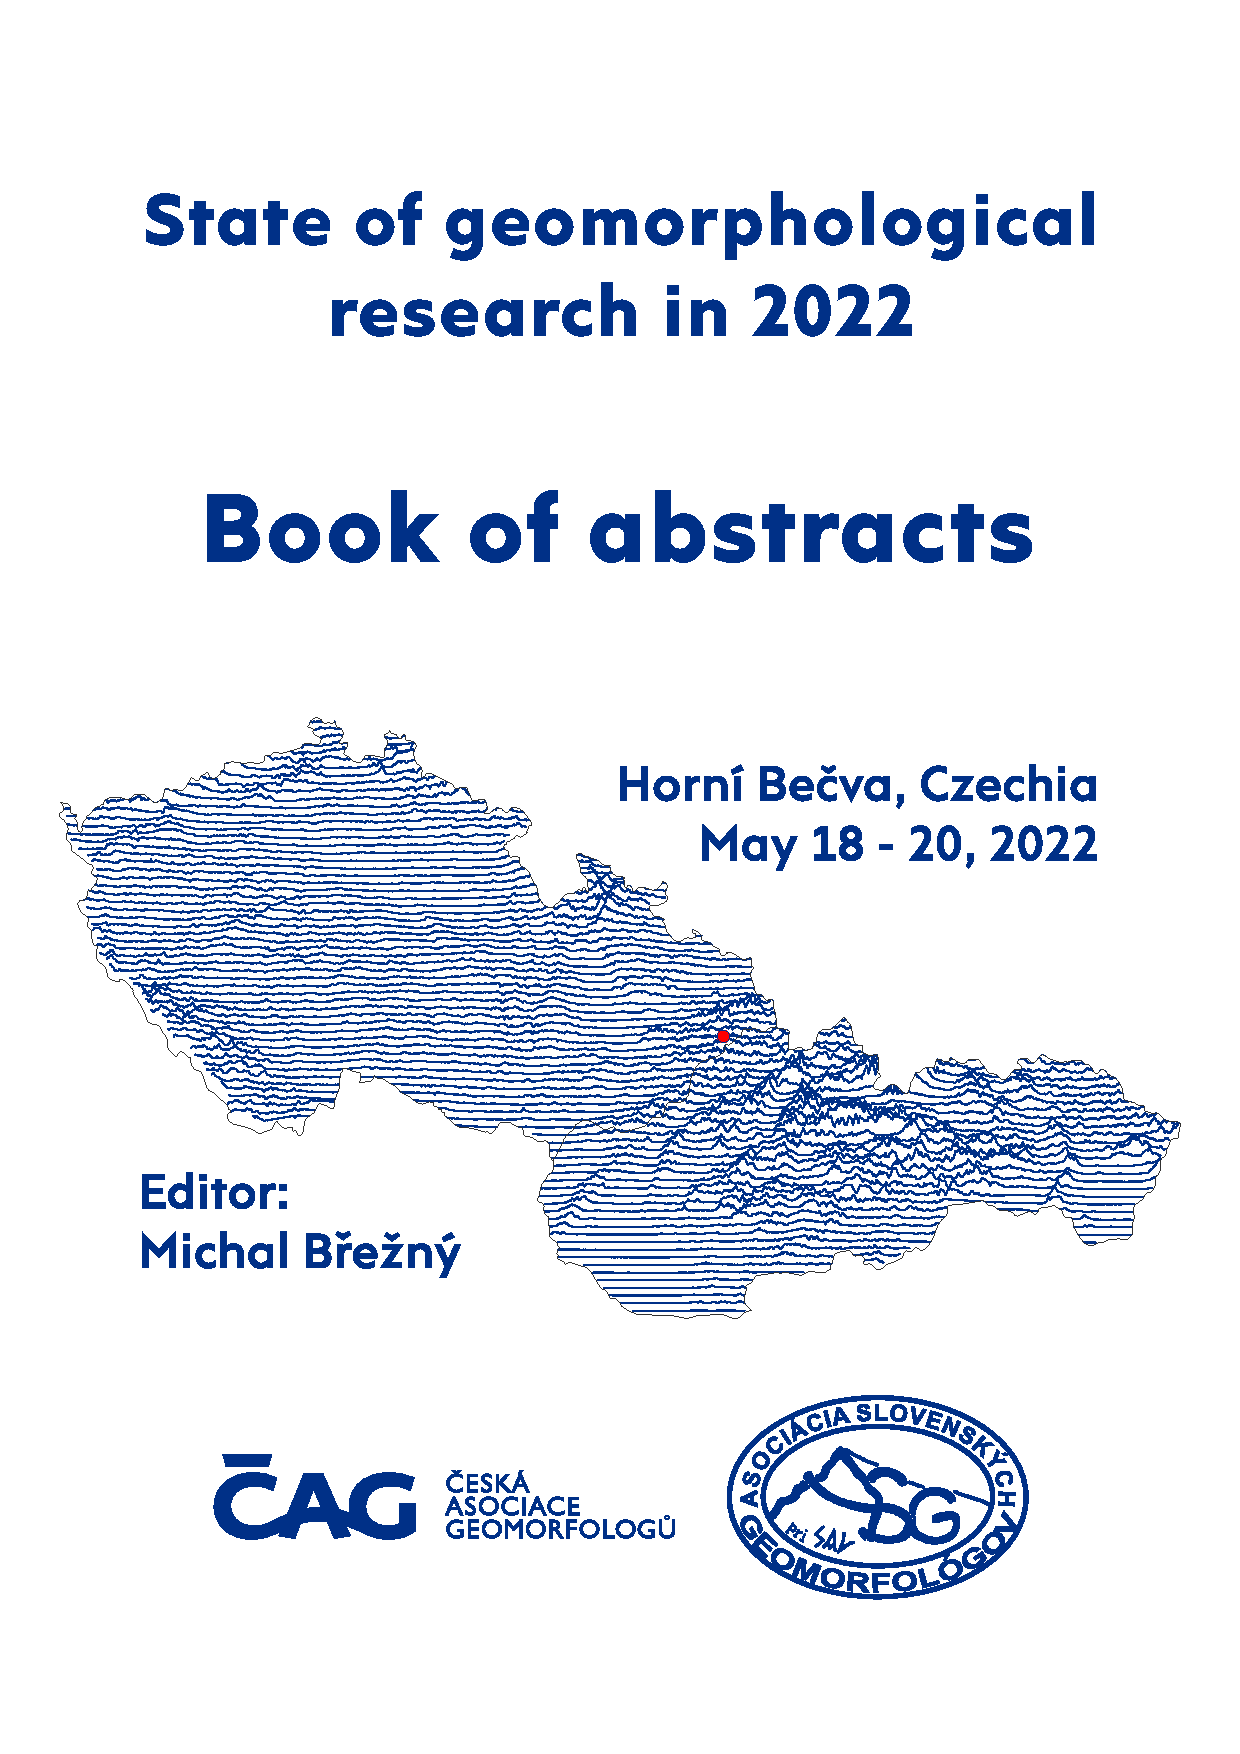
\includepdf{images/cover.pdf} % The cover for the booklet is included as a whole-page image, it can be a PDF or an image file but must be the same dimensions as the paper size

%----------------------------------------------------------------------------------------
%	 INFORMATION/COPYRIGHT PAGE
%----------------------------------------------------------------------------------------

\thispagestyle{empty} % Suppress headers and footers on this page

~\vfill % Push text down
% TODO: \usepackage{graphicx} required


\begin{center}	
\vspace{2em}
Book of abstracts\\
May 18 – 20, 2022 in Horní Bečva (Czech Republic)\\
\vspace{2em}
Editor: Michal Břežný\\ \vspace{2em}
The contributions contained in this publication have not undergone language and typographical editing. The authors are responsible for the linguistic and content quality of the texts.
\\ \vspace{2em}

Publisher: University of Ostrava, Ostrava \\\vspace{2em}

© 2022 Michal Břežný\\
\vspace{2em}
ISBN xxxxxxxxx\\

\vspace{5em}




%	This is the short version of the booklet for print use. \\ Full abstracts with all authors, references, and figures can be found at:\\ \url{https://amcosconference.com/}

This booklet is created using \LaTeX{} template which is based on the original version at:\\ \url{https://github.com/maximelucas/AMCOS\_booklet}
\end{center}



\newpage

%----------------------------------------------------------------------------------------
%	 TABLE OF CONTENTS
%----------------------------------------------------------------------------------------

\tableofcontents

%----------------------------------------------------------------------------------------
%	 ABOUT CONFERENCE
%----------------------------------------------------------------------------------------

\chapter{About}
\section{State of geomorphological research in 2022}
\noindent
State of geomorphological research in 2022 is organised bilaterally and should be perceived as the common conference of both Czech Association of Geomorphologists (\url{http://geomorfologie.eu}) and Association of Slovak Geomorphologists (\url{http://www.asg.sav.sk/}). Considering the 2-year pause due to the world pandemics, it is a round anniversary (20\textsuperscript{th} in the line of meetings started in 2000) for the Czech Association of Geomorphologists, and it is also the 11\textsuperscript{th} biennial meeting for the Association of Slovak Geomorphologists.

The thematic scope of the conference traditionally covers all geomorphological disciplines as well as those of related geosciences. 

\vspace{5em}
\section{Organizing committee}

\begin{flushleft}
	\begin{tabular}{l l l}
	RNDr. Veronika Kapustová, Ph.D. & Ing. Anna Kidová, PhD. & prof. RNDr. Tomáš Pánek, Ph.D.\\
	Mgr. Radek Tichavský, Ph.D. & RNDr. Jan Lenart, Ph.D. & doc. RNDr. Tomáš Galia, Ph.D.\\
	RNDr. Václav Škarpich, Ph.D. & Mgr. Michal Břežný, Ph.D. & doc. RNDr. Jan Hradecký, Ph.D.\\
	prof. RNDr. Karel Šilhán, Ph.D. & Mgr. Ján Novotný, PhD. & Mgr. Miloš Rusnák, PhD.\\
	Mgr. Zuzana Połedniková & Mgr. Adriana Holušová & Mgr. Vladimír Chalupa\\
	Mgr. Lukáš Vaverka & Mgr. Andrea Fabiánová & Mgr. Andrius Toločka 
	
	\end{tabular}
\end{flushleft}


\section{Organising institutions:}
\noindent
Czech Association of Geomorphologists\\
Association of Slovak Geomorphologists\\
Department of Physical Geography and Geoecology, Faculty of Science, University of Ostrava\\
Institute of Geography, Slovak Academy of Sciences
\begin{figure}[h]
	\centering
	
\includegraphics[width=1\linewidth]{images/geomorfologie-logolink}
\end{figure}

\newpage
% TODO: \usepackage{graphicx} required
\chapter{Under the auspices}
\begin{figure}[!htb]
	\centering
	\includegraphics[width=0.9\linewidth]{"images/logos/Partnerlogos/2022 04 25 záštita ČGS geomorfologové 1"}
\end{figure}


%----------------------------------------------------------------------------------------
%	 TIMETABLE
%----------------------------------------------------------------------------------------

\chapter{Timetable}

\section{Preconference workshop}

\begin{longtable}{|C{0.15\linewidth}| C{0.04\linewidth}|  C{0.3\linewidth} C{0.0\linewidth} C{0.4\linewidth}|}\hline	
	\eventtype{}{Tuesday May 17, 2022}
	\tablebreak{12:00--13:00}{Arrival/accommodation of the participants}
	\tablebreak{13:00--17:00}{Field survey and data acquisition on the Bečva River}
	\tablebreak{17:00--19:00}{Data processing}
	\eventtype{}{Wednesday May 18, 2022}
	\tablebreak{9:00--12:00}{Data processing and modelling, presentation of the results}

\end{longtable}

\section{Wednesday May 18, 2022}
\begin{longtable}{|C{0.15\linewidth}| C{0.04\linewidth}|  C{0.3\linewidth} C{0.0\linewidth} C{0.4\linewidth}|}\hline	
	\tablebreak{9:00--13:00}{Registration}
	\tablebreak{13:00}{Conference opening, invited lectures}
	\tablebreak{15:30}{Oral presentations}
	\tablebreak{17:00}{Poster session}
	\tablebreak{19:00}{Plenary meeting of the Czech Association of Geomorphologists}
	\tablebreak{19:00}{Plenary meeting of the Association of Slovak Geomorphologists}
\end{longtable}

\section{Thursday May 19, 2022}
\begin{longtable}{|C{0.15\linewidth}| C{0.04\linewidth}|  C{0.3\linewidth} C{0.0\linewidth} C{0.4\linewidth}|}\hline	
	\tablebreak{8:30--17:00}{Oral presentations}
	\tablebreak{17:00}{Poster session}
	\tablebreak{20:00}{Closing ceremony, Festive dinner}
\end{longtable}

\section{Friday May 20, 2022}
\begin{longtable}{|C{0.15\linewidth}| C{0.04\linewidth}|  C{0.3\linewidth} C{0.0\linewidth} C{0.4\linewidth}|}\hline	
	\tablebreak{8:30--16:00}{Conference field trip}
\end{longtable}

\newpage

%------------------------------------------------
%
%\section{Wednesday, 21 of March}
%
%\begin{longtable}{|C{0.15\linewidth}| C{0.04\linewidth}|  C{0.3\linewidth} C{0.0\linewidth} C{0.4\linewidth}|}\hline	
%	\IS{9:00-9:40}{Hiroya Sato}{Tokyo, Japan}{Title of invited speaker}
%	\CT{9:40-10:10}{Marc Fournier}{Brussels, Belgium}{Title of contributed talk}
%	\IS{10:10--12:45}{Hiroya Sato}{Tokyo, Japan}{Title of invited speaker}
%	\tablebreak{10:45--11:10}{Coffee}
%	%odor
%	\CT{11:10--11:40}{Marc Jansen}{Amsterdam, The Netherlands}{Title of contributed talk and references and a figure}
%	\CT{11:40--12:10}{Marc Jansen}{Amsterdam, The Netherlands}{Title of contributed talk and references and a figure}
%	\IS{12:10--12:45}{Hiroya Sato}{Tokyo, Japan}{Title of invited speaker}
%	\tablebreak{12:45--14:00}{Lunch}
%	\CT{14:00--14:30}{Marc Fournier}{Brussels, Belgium}{Title of contributed talk}
%	\CT{14:30-15:00}{Marc Fournier}{Brussels, Belgium}{Title of contributed talk}
%	\eventtype{16:30--18:00}{Excursion}
%	\eventtype{20:00}{Conference Dinner}
%\end{longtable}

%------------------------------------------------
%\begin{longtable}{|C{0.15\linewidth}| C{0.04\linewidth}|  C{0.3\linewidth} C{0.0\linewidth} C{0.4\linewidth}|}\hline	
%	\IS{9:00 -- 9:40}{Hiroya Sato}{Tokyo, Japan}{Title of invited speaker}
%	\IS{9:40--10:20}{Hiroya Sato}{Tokyo, Japan}{Title of invited speaker}
%	\IT{10:20--10:45}{Franck Schmidt}{Munich, Germany}{A special talk about diversity in science}
%	\tablebreak{10:45--11:10}{Coffee}
%	\CT{11:10-11:40}{Marc Jansen}{Amsterdam, The Netherlands}{Title of contributed talk and references and a figure}
%	\KL{11:40--12:35}{Leon Tremblay}{Montreal, Canada}{Title of a keynote lecture}
%	\eventtype{12:35--12:45}{Poster Prize \& Conclusion}
%	\tablebreak{12:45--14:00}{Lunch}
%\end{longtable}

%----------------------------------------------------------------------------------------
%	 LIST OF TALK ABSTRACTS
%----------------------------------------------------------------------------------------

% Abstract template
%\abstract
%	{} % Title
%	{} % Author(s)
%	{} % Tag, can be: empty, \KLtag (keynote lecture), \IStag (invited speaker), \CTtag (contributed talk) or \ITtag (invited talk)
%	{} % Affiliation(s)
%	{} % Abstract text

\chapter{List of Abstracts}

%
%start of abstract
%\abstract
%{} % Title
%{} %short author -- toc
%{\textsuperscript{1}*} % Author(s)
%{\KLtag} % Tag, can be: empty, \KLtag (keynote lecture), \IStag (invited speaker), \CTtag (contributed talk) or \ITtag (invited talk)
%{
%	\textsuperscript{1}
%	\textsuperscript{2}
%	\textsuperscript{3}
%}
%} % Affiliation(s)
%{}  %e-mail
%{}%keywords
%{
%}%abstract
%{
%}%references
%end of abstract

%%%%%%%%%%%%%%%%%%%%%%%%%%%%%%%%%%%%%%%%%%%%%%%%%%%%%%%%%%%%%%%%%%%%%%%%%%%%%%%%%%%%%%%%%%%%%%
%start of abstract
\abstract
{Dendrogeomorphic Dating in the Ostrava-Karviná Mining Landscape: Processes, Events, Responses} % Title
{Tichavský et al.} %short author -- toc
{Radek Tichavský\textsuperscript{1}*, Andrea Fabiánová\textsuperscript{1}, Eva Jiránková\textsuperscript{2}, Jan Lenart\textsuperscript{1}, Lucie Polášková\textsuperscript{1}, \\Radim Tolasz\textsuperscript{3}
} % Author(s)
{\TLtag} % Tag, can be: empty, \KLtag (keynote lecture), \IStag (invited speaker), \CTtag (contributed talk) or \ITtag (invited talk)
{
\textsuperscript{1}Department of Physical Geography and Geoecology, Faculty of Science, University of Ostrava, Chittussiho 10, 710 00 Ostrava, Slezská Ostrava, Czech Republic\\
\textsuperscript{2}Institute of Geonics of the Czech Academy of Sciences, Studentská 1768, 708 00 Ostrava, Czech Republic\\
\textsuperscript{3}Czech Hydrometeorological Institute, Na Šabatce 17, 143 06 Praha 4, Czech Republic
} % Affiliation(s)
{radek.tichavsky@osu.cz}  %e-mail
{mining landscape, dendrogeomorphology, subsidence, landslide, compression wood, Ostrava-Karviná mining district}%keywords
{Mining-induced subsidence is a worldwide environmental problem that leads to damage to infrastructure and property; thus, knowledge of its past–recent development is critically needed during land-use planning. We dated the activity of gravitational processes related to mining-induced subsidence using dendrogeomorphic methods at four sites in the Upper Silesian Coal Basin near the former mines of the Karviná mining district. The landslide/subsidence sites were characterised by scarps, rotated blocks, stepped relief with grabens, pressure folds, and shallow movements within landslide toes or within flat undulating relief. Based on 644 increment cores from 161 trees, we were able to identify subsidence/landslide activity, with the most frequent responses occurring from the late 1950s to the early 1970s and from 2005 to 2011. The highest number of tree ring records dates back to 1973. Moreover, more than 30\% of tilted trees from the landslide sites created compression wood at multiple directions indicated complex deformations. At the other sites, the occasional occurrence of single rings with isolated compression wood was included as a possible indicator of events due to frequent coincidence with common series of compression wood. A comparison of tree-ring-based chronology with in situ monitoring revealed good synchronicity with the periods of increased subsidence rates (between 1 and 3 m.year\textsuperscript{−1}). In addition, not only mining operations, but also the occurrence of extreme rainfall seems to be responsible for the recent surface activity. We identified that the 3-year precipitation and the Simple daily intensity index were significantly higher during event years at the site with a flatter topography and clay soils (p=0.02 and 0.01, respectively). Since dendrogeomorphic research on subsidence is influenced by multiple factors, including geological settings, soil conditions, or surface morphology, future research should focus on small research plots that provide detailed tree, surface, and subsurface characteristics. In addition, another challenge is to compare broadleaved and coniferous trees in terms of their sensitivity to recording subsidence movements on the same geomorphic forms.
}%abstract
{}%references
%end of abstract



%start of abstract
\abstract
{Flash Flood Simulation in the Urbanised Catchment: A Case Study of Bratislava–Karlova Ves} % Title
{Rusinko a Horáčková} %short author -- toc
{Adam Rusinko\textsuperscript{1}*, Šárka Horáčková$^2$} % Author(s)
{\KLtag} % Tag, can be: empty, \KLtag (keynote lecture), \IStag (invited speaker), \CTtag (contributed talk) or \ITtag (invited talk)
{
\textsuperscript{1}Faculty of Natural Sciences, Comenius University, Bratislava, Slovakia\\
\textsuperscript{2}Institute of Geography, Slovak Academy of Sciences, Bratislava, Slovakia
} % Affiliation(s)
{adam.rusinko@uniba.sk}  %e-mail
{Čierny potok stream, flash flood, GRASS GIS, LiDAR, CORINE Land Cover, Bratislava}%keywords
{Flash floods are a dangerous phenomenon that usually affects small drainage basins. They are primarily initiated in the upper parts of the slopes, but their injuring effects are manifested mostly in residential areas, where underground channelized streams disappeared from the surface. Therefore, there are not precise data about stream water levels available and only using surface runoff modelling is possible to simulate what happened during flash floods. Karlova Ves (Bratislava city District), formerly a small viniculture village, was threatened by floods (most probably including those of pluvial type) in the history. In this paper, we simulate surface runoff of a flash flood that occurred in the summer of 2014 in the catchment of Čierny potok using r.sim.water module in GRASS GIS. The flood in August 2014 was reported as with the highest rainfall per hour \textasciitilde40 during the time of local meteorological measurements. Current orthophotomap was used to classify CLC land cover classes, which were assigned the value of the Manning’s roughness coefficient and infiltration rate. The topography was expressed by DTM from high resolution LiDAR data. Our preliminary results indicate that land cover and land use are the essential factors influencing flash floods initiation, although the main driver in lower infiltration and change in flow direction is caused by urbanisation and high proportion of impervious areas. The simulation using r.sim.water module showed that during 60-minute extreme rainfall (40mm/hr) a surface runoff can reach a water depth up to 2 meters in terrain depressions by maximum discharge of 25 cubic meters per second. Natural urban areas revitalisation with increasing the vegetation cover in the areas prone to water flow and accumulation during higher rainfalls helps to prevent the damage caused by floods.
}%abstract
{Alizadehtazi B, DiGiovanni K, Foti R, Morin T, Shetty N H, Montalto F A, Sgurian P L (2016) Comparison of Observed Infiltration Rates of Different Permeable Urban Surfaces Using a Cornell Sprinkle Infiltrometer. Journal of Hydrologic Engineering 21(7): 06016003-1.

Hofierka J, Knutová M (2015) Simulating aspects of a flash flood using the Monte Carlo method and GRASS GIS: a case study of the Malá Svinka Basin (Slovakia). Open Geosciences 7(1): 118-125.

Lapin M, Mikulová K, Pecho J, Šťastný P (2019) Súčasná klimatická charakteristika MČ Bratislava – Karlova Ves a popis scenárov a dopadov zmeny klímy na riešené územie. SHMÚ, Bratislava.

Oťaheľ J, Feranec J, Kopecká M, Falťan V (2017) Modifikácia metódy CORINE Land Cover a legenda pre identifikáciu a zaznamenávanie tried krajinnej pokrývky v mierke 1:10 000 na báze príkladových štúdií z územia Slovenska. Geografický časopis 69(3): 189-224.

Prokešová R, Horáčková Š, Snopková Z (2022) Surface runoff response to long-term land use changes: Spatial rearrangement of runoff-generating areas reveals a shift in flash flood drivers. Science of the Total Environment 815: 151591.

Hydrology in GRASS GIS: A tutorial on hydrological modeling and simulation in GRASS GIS, \url{https://baharmon.github.io/hydrology-in-grass} cited in January 15, 2022

Letecké laserové skenovanie a DMR 5.0, \url{https://www.geoportal.sk/sk/zbgis/lls-dmr} cited in October 12, 2021
}%references
%end of abstract

%start of abstract
\abstract
{Long-Term Monitoring of the Recruitment and Dynamics of Large Wood in Kamienica Stream, Polish Carpathians} % Title
{Mikuś and Wyżga} %short author -- toc
{Paweł Mikuś, Bartłomiej Wyżga} % Author(s)
{\TLtag} % Tag, can be: empty, \KLtag (keynote lecture), \IStag (invited speaker), \CTtag (contributed talk) or \ITtag (invited talk)
{Institute of Nature Conservation, Polish Academy of Sciences, Kraków, Poland
} % Affiliation(s)
{mikus@iop.krakow.pl}  %e-mail
{large wood, wood dynamics, wood monitoring, wood inventory, Polish Carpathians}%keywords
{Quantifying wood delivery and mobility in small mountain streams requires long-term and repeatable observations, so far very scarcely described. Recently, observations using a number of remote sensing methods have gained popularity. However, classical methods of fieldwork still seem to be indispensable in more detailed studies. Such observations were conducted on the length of 8.7 km of the upper course of Kamienica Stream, Polish Carpathians, where recent bark beetle infestation of riparian spruce forest might have considerably increased the delivery of fallen trees to the channel. This part of the stream course is located in the Gorce Mountains National Park and large wood is not removed from the stream under the national park regulations.

In October 2009, numbered metal plates were installed on 429 trees growing along three stream sections located 2500–2950 m (section A), 4000–4450 m (section B) and 7850–8300 m (section C) from the stream source. Different metals were used in each section to allow for finding tagged trees with a metal detector in case the plates on them are inaccessible. The monitoring of standing and fallen trees tagged with metal plates has been conducted a few times per year, especially after heavy rainfall and windstorms. Moreover, the mode of location and the degree of decay of wood pieces stored in the study reach were determined in 2012.

During twelve years of observations, 111 trees (26\% of the tagged sample) were supplied to the stream as a result of bank erosion, windthrow of living trees or those killed by bark beetle infestation, snow overload and landslides. In October 2009, 80 cm of wet snow fell in two days and snow overload caused breaking of two tagged trees. Five events with high water stage occurred in May 2010, May 2014, July 2016, May 2018 and May 2019. Those from 2016 and 2018 can be considered as major floods as they caused significant channel changes and damage to local infrastructure. About half of trees supplied to the channel were not transported, and numerous wood dams occurring in the stream limited transport of any fallen trees. Forty-six fallen tagged trees (48\%) were transported during some of the five floods. In sections A and B, mean distance of the displacement of tagged trees over the study period was small and did not exceed 32 m, whereas in section C it was a few times longer. As a result of the flood in 2010, three trees were displaced relatively short distances (Mean = 42 m, Max = 100 m) and retained in in-channel jams. A definitely larger flood from 2014 was marked only in the lowermost section C, where the wood occurring in the channel was crushed into small pieces and flushed out downstream. The flood of July 2016 was the only major flood in all study sections; during this event 11 trees were displaced a mean distance of 97 m (Max = 230 m). In May 2018, a major flood caused by heavy rainfall resulted in considerable bank erosion in the lowest study section. During this event, 41 trees from this section were recruited to the channel and transported (Mean = 275 m, Max = 1003 m), while no transport occurred in the other sections. As trees in the upstream sections remained practically untouched, the course of this flood showed a strongly localized occurrence of the triggering rainfall. A small flood in May 2019 did not displace any tagged trees occurring in the stream. 

A large wood inventory performed in 2012 indicated that in the second-order reach wood was relatively uniformly distributed among different location types (Wyżga et al., 2015), with logs with their top or bottom located in the channel being the most abundant (21\% of all wood pieces). Moreover, near-perpendicular orientation of wood pieces in relation to the channel axis prevailed in the reach (Mikuś et al., 2016). All this indicates a negligible role of transport and redistribution of wood, which was predominantly retained where it fell. This reach was typified by the largest proportion of logs forming wood dams (12\%) and spanning the channel (10\%) among the study reaches, which can be attributed to the relatively large length of wood pieces in relation to channel width. The third-order reach was characterized by a similar pattern of wood location as the second-order reach. It was distinguished by only one feature: a small amount of wood spanning the channel. In the fourth-order reach, large wood spanning the channel was very scarce because of larger stream width and considerably larger flood discharges. Here, large wood was predominantly retained along channel margins (41\%), on gravel bars (19\%), and with only the top or bottom located in the channel (17\%). This reach was typified by variable orientation of wood pieces in relation to the channel axis, with a proportion of the pieces being apparently reoriented by the stream current. Most of wood pieces were shorter than channel width, as they originated from the breakage of trees into smaller fragments during their fall to the channel or transport by flood flows. 

The inventory also indicated that in the second-order reach of Kamienica, 16\% of wood pieces were in a relatively good condition, representing class 1 and 2 of wood decay, whereas a more advanced degree of decomposition, typical of class 3 and 4, typified 84\% of pieces. In the third-order stream reach, this distribution was more even, with 41\% of pieces representing class 1 and 2 of wood decay, and 59\% class 3 and 4. In the fourth-order reach, classes 1 and 2 constituted 31\% of all wood pieces, and 69\% had typical features of classes 3 and 4.

To conclude, large wood is recruited to the upper course of Kamienica Stream by a few processes, with bank erosion and windthrow having been most effective during 12 years of monitoring. Large wood was recruited to the stream only during high-intensity meteorological and hydrological events. With 22\% of tagged trees recruited to the channel during 12 years, the rate of turnover of the riparian trees was estimated at 45 years. As the riparian area supports trees with ages up to ~160 years, the rate evidences substantial intensification of large wood recruitment to the channel in the recent period resulting from bark beetle infestation of riparian trees. The mobility of wood in the stream increases downstream because of increasing flood discharges and the decreasing ability of fallen trees to anchor on the banks of increasingly wide channel. Wood is transported longer distances only during major floods, which tend to deposit wood pieces along channel margins and on gravel bars, where wood is subjected to relatively rapid decomposition under subaerial conditions. During a subsequent large flood, most wood pieces already occurring in the channel are thus likely to rapidly disintegrate, rather than being flushed out downstream. Thus, large wood retained in the upper stream course does not constitute an important flood hazard to downstream, inhabited valley reaches.
}%abstract
{Wyżga B, Zawiejska J, Mikuś P, Kaczka RJ (2015) Contrasting patterns of wood storage in mountain watercourses narrower and wider than the height of riparian trees, Geomorphology, 228, 275-285.  

Mikuś P, Wyżga B, Ruiz-Villanueva V, Zawiejska J, Kaczka RJ, Stoffel M (2016) Methods to assess large wood dynamics and the associated flood hazard in Polish Carpathian watercourses of different size. In: Kundzewicz ZW, et al. (eds.), Flood Risk in the Upper Vistula Basin. Springer, Cham, pp. 77-101.
}%references
%end of abstract


%start of abstract
\abstract
{Geomorphological Approach to Identification of Flood Hazard Hotspots Within Marginalized Roma Communities in Slovakia} % Title
{Jančovič and Kidová} %short author -- toc
{Marián Jančovič$^1$*, Anna Kidová$^1$} % Author(s)
{\KLtag} % Tag, can be: empty, \KLtag (keynote lecture), \IStag (invited speaker), \CTtag (contributed talk) or \ITtag (invited talk)
{$^1$) Institute of Geography, Slovak Academy of Sciences, Bratislava, Slovak Republic
} % Affiliation(s)
{geogjanc@savba.sk}  %e-mail
{flood hazard, height above nearest drainage, downslope distance to stream, Roma, segregation, Slovakia}%keywords
{Climate change has become one of the most acute problems of human society in recent decades. One of its manifestations is the worldwide increase in the intensity and frequency of extreme hydrological events, such as floods or droughts, which pose a direct threat to affected communities. In Slovakia, a significant number of settlements lie close to rivers and are therefore potentially exposed to flood hazard. Their local character also determines the uneven distribution of the threat they pose to individual communities. In addition, the unevenness of flood risk is reinforced by the different resilience and coping capacities of different social groups. Processes such as spatial segregation can then affect an excluded community twice. On the one hand, by pushing them into otherwise uninhabited floodplains, which are more susceptible to flooding and, on the other hand, by increasing their flood vulnerability. A prime example of spatial segregation in Slovakia are marginalised Roma communities (Rochovská a Rusnáková 2018). While the aspect of their increased vulnerability has been addressed in several studies (Filčák 2012; Harper, Steger, a Filčák 2009), the natural hazards that their environment poses to them has not been addressed so far. This presentation therefore focuses on the assessment of the flood hazard in those communities, based on their distances to nearest drainage, namely height above the nearest drainage (Rennó et al. 2008) and downslope distance to stream. Since the extent of the inudation zone is flow-dependent, the interpretation of the same distance differs for e.g., a mountain stream and a river of continental significance. We therefore attempted to minimize these differences by classification of streams based on flow accumulation. The geographic representation of marginalized Roma communities in the centroid form was derived from the buildings layer of the ZB GIS. In this way, we were able to automatically extract 120 out of 697 concentrations of segregated Roma population mentioned in the Atlas rómskych komunít (2019), which contains information only at the level of the cadastral territory of the municipality. By comparing this representation with the layer of flood occurrence in Slovak towns and villages between 1996-2019, we were able to identify hotspots of flood hazard within marginalised Roma communities, which will be addressed in future research.
	
This research was supported by the Science Grant Agency (VEGA) of the Ministry of Education of the Slovak Republic and the Slovak Academy of Sciences (02/0086/21).
}%abstract
{Filčák, Richard. 2012. “Environmental Justice and the Roma Settlements of Eastern Slovakia: Entitlements, Land and the Environmental Risks*”. Sociologicky Casopis 48 (3): 737–62. \doi{10.13060/00380288.2012.48.3.07}.

Harper, Krista, Tamara Steger, a Richard Filčák. 2009. “Environmental Justice and Roma Communities in Central and Eastern Europe”. Environmental Policy and Governance 19 (4): 251–68. \doi{10.1002/eet.511}.
	
Atlas rómskych komunít. 2019. Ministerstvo vnútra SR - Rómske komunity. \url{https://www.minv.sk/?atlas-romskych-komunit-2019}.

Rennó, Camilo Daleles, Antonio Donato Nobre, Luz Adriana Cuartas, João Vianei Soares, Martin G. Hodnett, Javier Tomasella, a Maarten J. Waterloo. 2008. “HAND, a New Terrain Descriptor Using SRTM-DEM: Mapping Terra-Firme Rainforest Environments in Amazonia”. Remote Sensing of Environment 112 (9): 3469–81. \doi{10.1016/j.rse.2008.03.018}.

Rochovská, Alena, a Jurina Rusnáková. 2018. “Poverty, Segregation and Social Exclusion of Roma Communities in Slovakia”. Bulletin of Geography. Socio-Economic Series 42 (42): 195–212. \doi{10.2478/bog-2018-0039}.
}%references
%end of abstract

%start of abstract
\abstract
{Transport, Retention and Geomorphic Impact of Large Wood in a Meandering River
} % Title
{Galia et al.} %short author -- toc
{Tomáš Galia$^1$*, Václav Škarpich$^1$, Matěj Horáček$^1$, Virginia Ruiz-Villanueva$^2$} % Author(s)
{\KLtag} % Tag, can be: empty, \KLtag (keynote lecture), \IStag (invited speaker), \CTtag (contributed talk) or \ITtag (invited talk)
{$^1$Faculty of Science, University of Ostrava, Ostrava, Czech Republic\\
$^2$Institute of Earth Surface Dynamics., University of Lausanne, Switzerland
} % Affiliation(s)
{tomas.galia@osu.cz}  %e-mail
{meandering river, large wood, river morphodynamics, Odra}%keywords
{Large wood (LW) is an integral part of rivers that supports habitat heterogeneity and biodiversity by its impact on flow hydraulics, channel morphodynamics and sediment transport (Gurnell et al., 2002). The majority of the research related to the geomorphic impact of LW was realised in wadeable channels, and we lack complex knowledge of the processes related to LW from large meandering rivers wider than the height of riparian trees (Wohl, 2017). This contribution presents the predictors of the interannual variability of the LW and its mobility during the 2016-2021 period in a 3.65 km long active meandering reach of Odra (Oder), Czechia (Galia et al., in review). We employed a repeated complete LW inventory and monitoring of tagged LW pieces. We found interannual variations in LW volumes (8.3-9.2 m3/ha), which did not allow us to develop any robust single model predicting LW volumes at the scale of meander bends (n = 14). Characteristics derived from riparian stands were found as important predictors of LW volumes. However, both positive and negative correlations between these characteristics and LW volumes were observed, which likely points to the complex recruitment-retention role of riparian stands. The dimensions of LW (i.e., length and diameter) together with the initial anchorage of the LW (i.e., its partial burial in sediments or racking by living trees or other LW) were determined as predictors of the LW mobility. The ratio between the LW channel width and the LW length was of greater importance for narrower channel segments, which points on some degree of equimobility of LW in the widest channel sections independently on the LW length. We also observed that local channel morphodynamics can be driven by the presence of single but stable LW. On the other hand, the noticeable spatiotemporal variation in jams between 2016 and 2021 was not only a product of the (suggested) frequent transport of relatively short LW pieces and related destruction of jams but also of the burial of jams in fine sediments during the process of channel migration. These field observations demonstrate the complex relationship between the channel morphodynamics and the biogeomorphic impact of vegetation in meandering rivers.
}%abstract
{Galia T, Horáček M, Ruiz-Villanueva V, Škarpich V (in review) Large wood retention and mobility in a large meandering river: insights from a 5-year monitoring in the Odra River (Czechia). Geomorphology.

Gurnell, AM, Piégay H, Swanson FJ, Gregory SV (2002) Large wood and fluvial processes. Freshwater Biology 47: 601–619.

Wohl E (2017) Bridging the gaps: An overview of wood across time and space in diverse rivers. Geomorphology 279: 3–26.
}%references
%end of abstract

%start of abstract
\abstract
{Verification of the "Čirá - Kopanina" fault zone using morphostructural analysis and geophysical methods} % Title
{Findžová et al.} %short author -- toc
{Leona Findžová$^1$, Petr Tábořík$^1,2$, Jakub Stemberk$^2$, Petra Štěpančíková$^2$} % Author(s)
{\KLtag} % Tag, can be: empty, \KLtag (keynote lecture), \IStag (invited speaker), \CTtag (contributed talk) or \ITtag (invited talk)
{$^1$Charles University, Faculty of Sciences, Prague\\
$^2$) Czech Academy of Sciences, Institute of Rock Structure and Mechanics, Prague
} % Affiliation(s)
{}  %e-mail
{Krušné hory Mts, fault zone, active tectonics, digital elevation model, morphostructural analysis, geophysical survey, electrical resistivity tomography}%keywords
{The aim of the research is to verify the existence of the "Čirá - Kopanina" fault zone in the western part of the Jindřichovice Highlands (Krušné hory Mts), which appears to be a potential source area for earthquake swarms at the boundary of the Cheb Basin and the Krušné hory crystalline complex. It is a possibly seismically active (seismogenic) structure and therefore a potentially active tectonic area. At the same time, it is a structure that is partly manifested on the surface, i.e. in the morphology of the terrain. The work builds on research already carried out in the area and aims to validate the hypothesis of a relatively less known fault structure that could predispose tectonic activity in the area. Thus, the research is focused on (i) characterizing the manifestations of the studied tectonic structure in the landscape by means of morphometric and morphostructural analyses of the area and (ii) subsequent verification of its occurrence directly in the field using geophysical methods. Morphometric and morphostructural analyses of the detailed digital elevation model (DMR 5G) were chosen as the basic methods of investigation, on the basis of which survey sites were selected for subsequent verification of the course of the searched fault zone using applied geophysical methods. Electrical resistivity tomography was selected as the primary method of geophysical survey as it is commonly used to verify the fault zones course. On the selected profile, the geoelectrical survey will also be complemented with seismic and gravity measurements. Preliminary results of the DEM analyses and initial geophysical measurements suggest that the investigated fault could indeed predispose the morphotectonic evolution of the area.
}%abstract
{}%references
%end of abstract

%start of abstract
\abstract
{Temporal Relationship of Deglaciation Phases and Palaeodischarges on the Catchment of River Maros, Central Europe} % Title
{Bartyik et al.} %short author -- toc
{Tamás Bartyik$^1*$, György Sipos$^1$, Dávid Filyó$^1$, Tímea Kiss$^1$, Petru Urdea$^2$ , Fabian Timofte$^2$} % Author(s)
{\KLtag} % Tag, can be: empty, \KLtag (keynote lecture), \IStag (invited speaker), \CTtag (contributed talk) or \ITtag (invited talk)
{$^1$Department of Geoinformatics, Physical and Environmental Geography, University of Szeged, Szeged, Hungary\\
$^2$ Department of Geography, West University of Timișoara, Timișoara, Romania
} % Affiliation(s)
{bartyikt@geo.u-szeged.hu}  %e-mail
{OSL dating, River Maros deglaciation, luminescence sensitivity, sediment delivery}%keywords
{River Maros has one of the largest alluvial fans in the Carpathian Basin. On the surface of the fan several very wide, braided channels can be identified, resembling increased discharges during the Late Glacial. In our study we investigated the activity period of the largest channel of them, formed under a bankfull discharge three times higher than present day values. Previous investigations dated the formation of the palaeochannel to the very end of the Pleistocene by dating a point bar series upstream of the selected site (Kiss et al. 2014). Our aim was to obtain further data on the activity period of the channel and to investigate temporal relationships between maximum palaeodischarges, deglaciation phases on the upland catchment and climatic amelioration during the Late Pleistocene. The age of sediment samples was determined by optically stimulated luminescence (OSL). The investigation of the luminescence properties of the quartz extracts also enabled the assessment of sediment delivery dynamics in comparison to other palaeochannels on the alluvial fan. 
OSL age results suggest that the activity of the channel is roughly coincident with, but slightly older than the previously determined ages, meaning that the main channel forming period started at 13.50\textpm0.94 ka and must have ended by 8.64\textpm0.82 ka (Kiss et al. 2015). This period cannot directly be related to the major phases of glacier retreat on the upland catchments, and in terms of other high discharge channels only the activity of one overlaps with a major deglaciation phase at \textasciitilde17--18 ka (Ruszkiczay-Rüdiger et al. 2016). Based on these, high palaeodischarges can be rather related to increased Late Glacial runoff, resulted by increasing precipitation and scarce vegetation cover on the catchment. Meanwhile, the quartz luminescence sensitivity of the investigated channel refers to fast sediment delivery from upland subcatchments. Therefore, the retreat of glaciers could affect alluvial processes on the lowland by increasing sediment availability, which contributed to the development of large braided palaeochannels.
}%abstract
{Kiss T, Sümeghy B, Sipos Gy (2014) Late Quaternary paleo-drainage reconstruction of the Maros River Alluvial Fan. Geomorphology 204, 49–60.
	
Kiss T, Hernesz P, Sümeghy B, Györgyövics K, Sipos Gy (2015) The evolution of the Great Hungarian Plain fluvial system - Fluvial processes in a subsiding area from the beginning of the Weichselian. Quaternary International 388, 142–155. 

Ruszkiczay-Rüdiger Zs, Kern Z, Urdea P, Braucher R, Madarász B, Schimmelpfennig I, ASTER TEAM (2016) Revised deglaciation history of the Pietrele-Stânişoara glacial complex, Retezat Mts, Southern Carpathians, Romania. Quaternary International 415, 216–229.
}%references
%end of abstract

%start of abstract
\abstract
{Geomorphic-Sedimentary Adjustment of a River Reach With Groynes to Channel Bypassing} % Title
{Lehotský et al.} %short author -- toc
{Milan Lehotský$^1$*, Miloš Rusnák$^1$, Šárka Horáčková$^1$, 
	Tomáš Štefanička$^2$, Jaroslav Kleň$^3$} % Author(s)
{\KLtag} % Tag, can be: empty, \KLtag (keynote lecture), \IStag (invited speaker), \CTtag (contributed talk) or \ITtag (invited talk)
{$^1$Department of Physical Geography, Geomorphology and Natural Hazards, Institute of Geography, Slovak Academy of Sciences, Štefánikova 49, 814 73 Bratislava, Slovakia, geoghora@savba.sk, geogmilo@savba.sk., geogleho@savba.sk \\
$^2$Department of Theoretical Geodesy, Slovak University of Technology in Bratislava, Radlinského 11, Block A, 810 05 Bratislava, Slovakia, e-mail: tomas.stefanicka@protonmail.com\\
$^3$Data Intelligence Engineer, DELL Technologies, Fazuľová 7, 81107 Bratislava, Slovakia  klen.jaro@gmail.com
} % Affiliation(s)
{geogleho@savba.sk}  %e-mail
{Gabcikovo Waterworks; spatio-temporal variability; groyne-induced bench; vertical accretion; conveyance; flood; Danube }%keywords
{The article is focused on the investigation of spatio-temporal variability of the vertical accretion thickness as the response of the Danube River reach to bypassing. Five groyne-induced benches (GIB) of the bypassed channel were developed after water diversion in 1992 and represent our study area. Their topography was created from LiDAR point cloud dataset and DEM models for tree time spans (for original gravel surface, for surface before flood 2013, surface after flood 2013) were calculated and the allostratigraphic approach was applied on 548 drilling probes at five GIB cross-sections.  Head, supra-platform, tail and back channel geomorphic units have been identified at each GIB. The accretion was influenced mostly by large flood events when the 100-yr contributed to the its total volume by almost 26\%. The head geomorphic unit, as the main impact zone on the stream, exhibits the highest median values of vertical accretion in time and space. The median of the vertical accretion thickness does not decrease with height above mean channel water level and the thickness of accretion varied likely due to variability of the vegetation cover conditioning variable hydraulic conditions. The bend setting, lower radius of curvature, lower width-depth ratio, connectivity with side arm and well-developed alternate bench upstream conditioned higher vertical accretion of the benches and its slight migration downstream. Moreover, higher portion of the area was formed as backwater geomorphic unit. The comparison of sediment depth over time spans (22 and 20 years and a large flood event) allowed us to conclude that the it is spatially variable by individual GIB, however its sedimentation trend over time is the same.
	
Ackowledgements: This research was supported by the Scientific Grant Agency of the Ministry of Education, Science and Sport of the Slovak Republic (VEGA 2/0086/21). We appreciate LiDAR data provided by National Forest Centre in Zvolen.
	}%abstract
{}%references
%end of abstract

\abstract
{Changes of Fluvial Processes Caused by the Restoration of
	an Incised Mountain Stream
} % Title
{Wyżga et al.} %short author -- toc
{Bartłomiej Wyżga$^1$*, Maciej Liro$^1$, Paweł Mikuś$^1$, Artur Radecki-Pawlik$^2$, Józef Jeleński$^3$, Joanna Zawiejska$^4$, Karol Plesiński$^5$} % Author(s)
{\KLtag} % Tag, can be: empty, \KLtag (keynote lecture), \IStag (invited speaker), \CTtag (contributed talk) or \ITtag (invited talk)
{$^1$Institute of Nature Conservation, Polish Academy of Sciences, Kraków, Poland\\
$^2$Faculty of Civil Engineering, Cracow University of Technology, Kraków, Poland\\
$^3$‘Upper Raba River Spawning Grounds’ Project Coordinator, Myślenice, Poland\\
$^4$Institute of Geography, Pedagogical University of Cracow, Kraków, Poland\\
$^5$Department of Hydraulic Engineering, University of Agriculture in Kraków, Poland
} % Affiliation(s)
{wyzga@iop.krakow.pl}  %e-mail
{channel incision, stream restoration, block ramp, hydraulic modelling, floodwater retention, hydromorphological quality, Polish Carpathians}%keywords
{Construction of a high check dam on mountain Krzczonówka Stream, Polish Carpathians, in the mid-20th century resulted in a number of detrimental changes to the downstream reach. Entrapment of bed material behind the dam caused long-lasting sediment starvation of the downstream reach leading to channel incision and transformation of the former alluvial channel into a bedrock-alluvial or bedrock channel. High flow capacity of the incised channel was reflected in high velocity and bed shear stress associated with flood discharges of given recurrence interval, which prevented in-channel deposition of bed material in case of its delivery from the upstream reach. Concentration of flood flows in the incised channel considerably reduced floodwater retention in the floodplain area, hence contributing to rapid downstream passage of flood waves and increase in their peak discharges. Finally, hydromorphological quality of the stream was degraded as a result of morphological, sedimentary and hydraulic changes in the downstream reach coupled with the disruption of longitudinal stream continuity for aquatic biota caused by the check dam. 

In 2012 a restoration project was initiated to lower the check dam and make the structure passable for fish. To trap the sediment flushed out from the dam reservoir in the incised channel, several block ramps were constructed in 2013, before the onset of the works on the check dam. The check dam was lowered in 2014 and when the works were underway, a 7-year flood occurred on the stream, flushing out a considerable amount of sediment from the dam reservoir. The sediment was efficiently trapped by the block ramps in the downstream reach. This study aims at investigating how the environmental problems caused by the long-term sediment starvation of the stream were mitigated by the restoration works. 

Channel morphology was surveyed after the installation of block ramps but with still unmodified check dam (2013) and after the check-dam lowering (2015). These surveys were done in 10 cross-sections delimited in the downstream reach of the stream. Data about cross-sectional stream morphology, channel slope as well as channel and floodplain roughness were used in hydraulic modelling of flood conditions typifying the stream before (2013) and after (2015) deposition of the sediment trapped by block ramps. The modelling was performed using HEC-RAS software. Moreover, hydromorphological quality of the stream was evaluated in 2012 and 2015 according to the River Hydromorphological Quality method, which is especially suitable for the assessment of effects of river restoration activities (Hajdukiewicz et al., 2017). 

Deposition of the sediment flushed out from above the lowered check dam caused burying of the boulder ramps on the distance of 1.2 km from the dam, whereas the sediment wave reached 1.6 km from the dam. About 15650 m3 of bed material were retained in the stream, resulting in re-establishment of alluvial channel bed and an average aggradation of the channel bed by 0.50 m. Bed aggradation and the resultant increase in the elevation of low-flow water surface were relatively large close to the check dam, attaining maximum values of around 1 m at the distance of 440 m from the dam, and decreased in the downstream direction. As bed aggradation reduced flow capacity of the channel, unit stream power and bed shear stress in the channel zone of the stream decreased, with the largest decrease of these parameters by 36\% and 30\%, respectively, recorded for a 20-year flood. These changes were reflected in reduced competence of the stream, with the average reduction of entrainable grain size of bed material by 18\% for a 2-year flood and by 31\% for the 20-year flood. The reduction in flow capacity of the channel increased retention potential of the floodplain, i.e. a proportion of the total cross-sectional flow area in which floodwater would remain motionless, thus being temporarily retained on the floodplain (Wyżga, 1999; Czech et al., 2016). However, this effect was not statistically significant in the set of 10 study cross-section, but was relatively large where the channel bed aggraded substantially, while small in the cross-sections with a small increase in bed elevation. Before the restoration works, only 1 of the 5 evaluated stream cross-sections was classified as representing good hydromorphological quality, whereas after the works 4 cross-sections fell in this class of hydromorphological quality. The hydromorphological quality improvement mainly reflected changes in bed substrate, erosional and depositional channel features and longitudinal stream connectivity. 

To conclude, inventories performed before and after the restoration works demonstrated effectiveness of block ramps in mitigating problems in the physical functioning of an incised mountain stream. With the entrapment of bed material by block ramps, channel bed considerably aggraded and changed from the bedrock to an alluvial one. The bed aggradation significantly decreased bed shear stress and entrainable grain size of bed material. Floodwater retention in the floodplain area increased, although this effect was largely dependent on the amount of bed aggradation in the study cross-sections. The hydromorphological quality of the stream improved in 4 out of the 5 evaluated cross-sections, with 3 cross-sections being upgraded from moderate to good quality class. 
	
This study was prepared within the scope of Research Project 2019/33/B/ST10/00518 financed by the National Science Centre of Poland.
}%abstract
{Czech W (2016) Modelling the flooding capacity of a Polish Carpathian river: A comparison of constrained and free channel conditions. Geomorphology 272: 32–42. 
	
Hajdukiewicz H, Wyżga B, Zawiejska J, Amirowicz A, Oglęcki P, Radecki-Pawlik A (2017) Assessment of river hydromorphological quality for restoration purposes: an example of the application of RHQ method to a Polish Carpathian river. Acta Geophysica 65: 423–440. 

Wyżga B (1999) Estimating mean flow velocity in channel and floodplain areas and its use for explaining the pattern of overbank deposition and floodplain retention. Geomorphology 28: 281–297. 
}%references

\abstract
{Fluvial Habitat Assessment Using High-Resolution 3D Models} % Title
{Rusnák et al.} %short author -- toc
{Miloš Rusnák$^1$*, Peter Mihálik$^2$, Ján Sládek$^3$} % Author(s)
{\KLtag} % Tag, can be: empty, \KLtag (keynote lecture), \IStag (invited speaker), \CTtag (contributed talk) or \ITtag (invited talk)
{
$^1$Institute of Geography SAS, Bratislava, Slovakia\\
$^2$Faculty of Natural Sciences, Comenius University, Bratislava, Slovakia\\
$^3$Institute of Geography SAS, Bratislava; GEOTECH Bratislava, Slovakia\\
} % Affiliation(s)
{geogmilo@savba.sk}  %e-mail
{UAV, river channel, bathymetry, classification, fluvial habitats}%keywords
{The paper aims to create a detailed automatic classification of the river landscape habitats based on high-resolution data obtained by drones. We apply automatic classification of the floodplain landscape structure and in-channel physical habitats. As part of automated classification, we test the accuracy of pixel-based and object-oriented supervised classification, using data sets composed of traditional spectral characteristics (RGB) and the geometric properties of the point cloud. The channel bathymetry was identified by modelling the relationship between spectral parameters of the image and field measured water depth or by the correction of the photogrammetrically generated bathymetry model by the refraction coefficient. The accuracy of the automatic classification was evaluated based on KAPPA indices using the validation layer, and the RMSE error was used for bathymetric models. In total, we classify nine main classes of land cover: water; low vegetation (less than 0.5 m); medium vegetation (0.5 - 3 m); high vegetation (more than 3 m); gravel bar; flood facies; bedrock and LWD. The submerged physical morphology was divided into four classes based on water depth. For object-oriented classification on the data layer using only the colour spectrum RGB, the accuracy of vegetation classification was 98.1 \%. The water depth in the riverbed was identified based on a bathymetric model with a determination coefficient of 0.8161 and an RMSE error of 0.2419 m. The physical habitat in the river includes different continuums (grain size, water depth, topographic elevation and flow velocity) as a main physical river habitat parameter constituted by the flow regime (hydrology and hydraulics) and the physical template (fluvial sedimentology and geomorphology). Physical habitat parameters will be extracted from a detailed bathymetry model, reconstructing the channel bed structure, gravel bars and identifying habitat patterns essential for maintaining fish assemblage biodiversity. From hydraulic modelling, we used flow velocity. For final class mapping, we used velocity data, water depth and morphology unit classification (pool, glide, run, riffle). The research was supported by the Scientific Grant Agency VEGA, number 2/0086/21.
}%abstract
{}%references

\abstract
{Using Airborne Lidar Data for Detecting Anthropogenic Landforms in Poiplie Region} % Title
{Lieskovský et al.} %short author -- toc
{Juraj Lieskovský$^1$*, Dana Lieskovská$^1$, Tibor Lieskovský$^2$, Petra Gašparovičová$^1$} % Author(s)
{\KLtag} % Tag, can be: empty, \KLtag (keynote lecture), \IStag (invited speaker), \CTtag (contributed talk) or \ITtag (invited talk)
{$^1$Institute of Landscape Ecology, Slovak Academy of Sciences, Bratislava, Slovakia\\
$^2$Department of Theoretical Geodesy and Geoinformatics, Slovak University of Technology, Bratislava, Slovakia
} % Affiliation(s)
{juraj.lieskovsky@savba.sk}  %e-mail
{LiDAR, landscape palimpsest, Kiarov, Kováčovce, landscape archaeology, anthropogenic landforms}%keywords
{We present the use of Light Detection and Ranging  (LiDAR) data for mapping the anthropogenic landforms in Kiarov and Kováčovce villages, located in Poiplie region. The benefits of LiDAR are the speed of data acquisition on a landscape scale, the quality of its surface data, and its ability to identify macro- and micro-topographical features that are otherwise undetected by terrestrial surveys. LiDAR is now used for detailed topographical research in many disciplines including geomorphology. The area of Slovakia is being scanned from 2017 at a resolution of 20–30 points per square metre and is scheduled to be completed by 2023. 
	
For the interpolation of the LiDAR points to digital elevation model with resolution 25cm, we used points classified as ground and buildings. We applied the visualisation techniques based on a simple local relief model (Kokalj \& Hesse, 2017) but we also added a local dominance to relief curvature representation and also added a combination of slope steepness and sky view factor to relief contrast visualisation (Lieskovský et al., in press). We visually identified the topographic signatures of geomorphic anthropogenic landforms and consulted our findings with historical maps and aerial images. We followed the anthropogenic landform ontology proposed by Tarolli et al. (2019) and we categorized the landforms in the following categories: (1) ‘symbolic’ were represented by cemeteries and chapel; (2) ‘habitation’ were represented by habitation areas and dispersed settlements; (3) ‘transport and exchange’ were represented by paved and unpaved roads, including traces of roads that are not used anymore; (4) ‘subsistence’ were represented by traditional and socialistic agricultural terraces, house gardens, agricultural enterprises, vineyards and orchards and  hedgerows; (5) ‘mining’ were represented by surface mining pits (6) ‘water infrastructure’ consisted of melioration canals and artificial river bed of Ipel river; (7) ‘waste disposal’ was found in central part of Kováčovce cadastral area; and (8) ‘warfare infrastructure’ was represented by trenches and ditches from the Second World War.
}%abstract
{Kokalj Ž, Hesse R (2017) Airborne Laser Scanning Raster Data Visualization. Vol. 14. Prostor, Kraj, Čas. ZRC SAZU, Založba ZRC, Ljubljana

Lieskovský J, Lieskovský T, Hladíková K, Štefunková D, Hurajtová N (in press) Potential of Airborne LiDAR Data in Detecting Cultural Landscape Features in Slovakia. Landscape Research.

Tarolli P, Wenfang C, Giulia S, Damian E, and Erle C-E(2019) From Features to Fingerprints: A General Diagnostic Framework for Anthropogenic Geomorphology. Progress in Physical Geography: Earth and Environment 43, no. 1: 95–128.}%references

\abstract
{Large landslides along the eastern margin of Patagonian Ice Sheet: distribution, causes and timing} % Title
{Pánek et al.} %short author -- toc
{Tomáš Pánek$^1$, Michal Břežný$^1$, Elisabeth Schönfeldt$^2$, Veronika Kapustová$^1$, Diego Winocur$^3$, Rachel Smedley$^4$} % Author(s)
{\KLtag} % Tag, can be: empty, \KLtag (keynote lecture), \IStag (invited speaker), \CTtag (contributed talk) or \ITtag (invited talk)
{$^1$University of Ostrava, Department of Physical Geography and Geoecology, Chittussiho 10, Slezská Ostrava, Czech Republic \\
	$^2$University of Potsdam, Institute of Geosciences, Karl-Liebknecht-Straße 24-25, 14476, Potsdam, Germany \\
	$^3$Universidad de Buenos Aires, Facultad de Ciencias Exactas y Naturales, Departamento de Ciencias Geologicas, Intendente Güiraldes 2416, C1428EGA, CABA, Argentina \\
	$^4$University of Liverpool, Department of Geography and Planning, Chatham Street, Liverpool, L69 7ZT, UK} % Affiliation(s)
{tomas.panek@osu.cz}  %e-mail
{}%keywords
{Although ice retreat is widely considered to be an important factor in landslide origin, many links between deglaciation and slope instabilities are yet to be discovered. Here we focus on the origin and chronology of exceptionally large landslides situated along the eastern margin of the former Patagonian Ice Sheet (PIS). Accumulations of the largest rock avalanches in the former PIS territory are concentrated in the Lago Pueyrredón valley at the eastern foothills of the Patagonian Andes in Argentina. Long-runout landslides have formed along the rims of sedimentary and volcanic mesetas, but also on the slopes of moraines from the Last Glacial Maximum. At least two rock avalanches have volumes greater than 1 km\textsuperscript{3} and many other landslide accumulations have volumes in the order of tens to hundreds of million m\textsuperscript{3}. Using cross-cutting relationships with glacial and lacustrine sediments and using OSL and \textsuperscript{14}C dating, we found that the largest volume of landslides occurred between \textasciitilde17 and \textasciitilde11 ka. This period coincides with the most rapid phase of PIS retreat, the greatest intensity of glacial isostatic uplift, and the existence of a dropping glacial lake along the foothills of the Patagonian Andes. The position of paleoshorelines in the landslide bodies and, in many places, folded and thrusted lacustrine sediments at the contact with rock avalanche deposits indicate that the landslides collapsed directly into the glacial lake. Although the landslides along the former glacial lobe of Lago Pueyrredón continue today, they are at least an order of magnitude smaller than the rock and debris avalanches that occurred before the drainage of the glacial lake around 10-11 ka. Preliminary numerical modeling results indicate that large postglacial landslides may have been triggered by a combination of rapid sequential glacial lake drawdowns and seismicity due to glacial isostatic adjustment. We conclude that in addition to direct links such as glacial oversteepening, debuttressing and permafrost degradation, the retreat of ice sheets and the subsequent formation of transient large glacial lakes can fundamentally alter stability conditions, especially if the slopes are built by weak sedimentary and volcanic rocks.}%abstract
{}%references



\abstract
{Identification of benches and ledges within the braided-wandering floodplain formation} % Title
{Labaš, Peter and Anna Kidová} %short author -- toc
{Peter Labaš, Anna Kidová} % Author(s)
{\KLtag} % Tag, can be: empty, \KLtag (keynote lecture), \IStag (invited speaker), \CTtag (contributed talk) or \ITtag (invited talk)
{Department of Physical Geography, Geomorphology and Natural Hazards, Institute of Geography, Slovak Academy of Science, Štefánikova 49, 814 73 Bratislava} % Affiliation(s)
{geoglaba@savba.sk}  %e-mail
{meandering; river degradation; multi-temporal analysis; flood event; the Hornád River}%keywords
{At the turn of the 19\textsubscript{th} and 20\textsubscript{th} century, the Hornád River in Slovakia in its middle reach was typical by passing the Hornád basin, typical by several levels of river terases (Michaeli 2001), well-developed floodplains and water-gaps. The wide floodplains were characteristic by free meanders which had been in the 20\textsubscript{th} century affected by human interventions, peaked in the 50s. The anthropogenic impact resulted in channel shortening and narrowing, river sinuosity lowering, erosion-accumulation processes decreasing and free meanders loss. Additionally, the long-term discharge reduction had caused simplification of channel planform in stream sections without or with minimal anthropogenic impact. This trend was later abrupted by the flood event series in 2004, 2008 and 2010. The flood events were also documented as an important factor for a morphological change in the lower part of the Hornád River in Hungary (Kiss and Blanka, 2011; Kiss and Blanka, 2012). Environmentally changed conditions (anthropogenic impact and floods) on the 72 km long channel planform of the meandering Hornád River in Slovakia were observed on three types of river segments (natural, regulated, water-gap) by seven sets of data, including the second and third military survey and five ortophoto mosaics and aerial photos (1949, 1986, 2002, 2013, 2016). The Hornád River in the pre-regulation period was represented by a natural meandering river planform (45.8 \%) with a high occurrence of in-channel landforms, where the lateral bar area prevailed. At present, due to the simplification of the river channel planform, only 26 \% of the river segments with ongoing natural erosion-accumulation processes and the last two locations with free meanders on the middle reach of the Hornád River remained.
}%abstract
{Kiss, T. and Blanka, V. (2011) Effect of different water stages on bank erosion, case study on River Hernád, Hungary, Carpathian Journal of Earth and Environmental Sciences, 6(2), pp. 101-108
	
	Kiss, T. and Blanka, V. (2012) River channel response to climate- and human-induced hydrological changes: Case study on the meandering Hernád River, Hungary, Geomorphology, 175–176, pp. 115–125. doi: 10.1016/j.geomorph.2012.07.003.
	
	Labaš, P. and Kidová, A., (2022). Anthropogenic and environmental impacts on the recent morphological degradation of the meandering Hornád River, Geografický časopis,  74(2), in press
	
	Michaeli, E. (2001). Georeliéf hornádskej kotliny, Geografické práce, 9(2), 153 p.  
}%references

\abstract
{Identification of benches and ledges within the braided-wandering floodplain formation} % Title
{Labaš et al.} %short author -- toc
{Peter Labaš, Anna Kidová, Šárka Horáčková, Milan Lehotský, Miloš Rusnák
} % Author(s)
{\KLtag} % Tag, can be: empty, \KLtag (keynote lecture), \IStag (invited speaker), \CTtag (contributed talk) or \ITtag (invited talk)
{Department of Physical Geography, Geomorphology and Natural Hazards, Institute of Geography, Slovak Academy of Science, Štefánikova 49, 814 73 Bratislava} % Affiliation(s)
{geoglaba@savba.sk}  %e-mail
{braided-wandering river; floodplain evolution; benches; ledges; gravel-bed river}%keywords
{The Belá River in the north part of Slovakia represents a braided-wandering river system (Kidová et al., 2016) with repeatedly destroying and re-forming floodplain, as a result of lateral shifting of an active river zone of braided rivers (Haschenburger and Cowie, 2009). These processes depend on flood events and a large volume of sediment transportation. Benches as unstable (Erskine and Livingstone, 1999), fine sediment storage (Kemp, 2004; Vietz et al., 2005a, 2005b) are formed by flood events (Webb, Erskine a Dragovich, 2002) in the margin of the active river zone of the Belá River and they are also destroyed by another even larger flood events (Erskine a Peacock, 2002). However, in the last decades, we are able to observe changes in the magnitude of flood events and the volume of sediment transportation of the Belá River (Kidová, et al., 2016b). The changes caused a simplification of the river planform, leading to a better-developed mature floodplain. The benches in these parts are a well-preserved component of the floodplain. Moreover, local incision of the river channel led to more-level floodplain development with benches set into them. While incision forbids to another floodplain development results of its mutual effect with flood events are ledges, as a level of bank erosion (Lehotský et al., 2015). Following previous research supplemented by new field surveys we are focused to study of river floodplain evolution of the Belá River. In the end, it will be possible to formulate a process-oriented hypothesis of the recent lateral and vertical development of the floodplain.
}%abstract
{Erskine, W. D. and Livingstone, E. (1999) In-channel benches: the role of floods in their formation and destruction on bedrock confined rivers, Varieties of Fluvial Form, (January 1999), s. 445–475.

Erskine, W. D. and Peacock, C. T. (2002) Late holocene flood plain development following a cataclysmic flood, The Structure, Function and Management Implications of Fluvial Sedimentary Systems, (276), s. 177–184.

Haschenburger, J. K. and Cowie, M. (2009) Floodplain stages in the braided Ngaruroro River, New Zealand”, Geomorphology, 103(3), s. 466–475. \doi{10.1016/j.geomorph.2008.07.016}.

Kemp, J. (2004) Flood channel morphology of a quiet river, the Lachlan downstream from Cowra, southeastern Australia, Geomorphology, 60(1–2), s. 171–190. \doi{10.1016/j.geomorph.2003.07.007}.

Kidová, A., Lehotský, M. and Rusnák, M. (2016a) Geomorphic diversity in the braided-wandering Belá River, Slovak Carpathians, as a response to flood variability and environmental changes, Geomorphology, 272, s. 137–149.\doi{10.1016/j.geomorph.2016.01.002}.

Kidová, A., Lehotský, M. and Rusnák, M. (2016b) Morfologické zmeny a manažment divočiaco-migrujúceho vodného toku Belá, GEOMORPHOLOGIA SLOVACA ET BOHEMICA, 16(2), s. 60.

Lehotský, M., Kidová, A. and Rusnák, M. (2015) Slovensko-anglické názvoslovie morfológie vodných tokov, GEOMORPHOLOGIA SLOVACA et BOHEMICA, 15(1), s. 61.

Vietz, G., Stewardson, M. and Rutherfurd, I. (2005a) Not all benches are created equal: Proposing and field testing an in-channel river bench classification, v Proceedings of the 4th Australian Stream Management Conference, s. 629–635.

Vietz, G., Stewardson, M. and Rutherfurd, I. (2005b) Variability in river bench elevation and implications for environmental flow studies, v, s. 8.

Webb, A. A., Erskine, W. D. and Dragovich, D. (2002) Flood-driven formation and destruction of a forested flood plain and in-channel benches on a bedrock-confined stream: Wheeney Creek, southeast Australia, IAHS-AISH Publication, (276), s. 203–210.
}%references

\abstract
{Impact of Flood Events and Eurasian Beaver (Castor Fiber) Activity on Spontaneous Renaturalization of Łososina River in the Polish Western Carpathians} % Title
{Wąs and Gorczyca} %short author -- toc
{Joanna Wąs$^1$*, Elżbieta Gorczyca$^2$} % Author(s)
{\KLtag} % Tag, can be: empty, \KLtag (keynote lecture), \IStag (invited speaker), \CTtag (contributed talk) or \ITtag (invited talk)
{$^1$Institute of Geography and Spatial Organization, Polish Academy of Sciences\\
	$^2$Institute of Geography and Spatial Management, Jagiellonian University in Cracow} % Affiliation(s)
{joanna.was@zg.pan.krakow.pl}  %e-mail
{spontaneous renaturalization, river channel development, channel migration zone, flood, European Beaver (Castor fiber), Beskid Wyspowy Mts.}%keywords
{Rivers in Polish part of Carpathians are heavily modified. Valleys are urbanized, banks are enforced, channels are straightened and various types of barriers are employed to regulate the flow. All these alterations cause disturbance of natural morphodynamic processes and destruction of habitats. Anthropogenic pressure may also increase risks related to floods and droughts.

Contrary to the trends prevailing in the industrial era, more and more attention is now being paid to the negative effects of river regulation (e.g. Gregory, 2006). Growing awareness of the importance of preserving or restoring the natural state of rivers and water resources for the proper functioning of the environment and people leads to implementation of river restoration projects (e.g. Wohl et al., 2005). However, such actions are expensive and therefore not carried out on a large scale. That is why all factors that may cause renaturalization process to occur without technical treatment deserve special consideration.

Some rivers display tendencies to partially compensate for the disturbances via spontaneous changes of various parameters such as sinuosity and wideness (e.g. Bollati et al., 2014). When left not maintained training structures may deteriorate in time. Eventually such constructions collapses and therefore natural hydromorphological processes may be restored to some extent, especially with external help.

One of the key features characteristic for the multithread natural or semi-natural river is heterogeneity of the flow. Frequently such conditions are not met in regulated part of rivers. To help restore natural state we may employ various expensive technical measures or we can let it be done by the beavers (Castor fiber) which are known for their ability to create heterogeneous (aquatic and terrestrial) habitats (e.g. Rosell et al., 2005).

We examined channel development of gravel-bed river Łososina in Beskid Wyspowy Mts. (Western Carpathians). During this project both of these factors were found to be important for spontaneous renaturalization. Analyses were conducted using data concerning river training made by RZGW (1973–2015), orthophotos, aerial photos, topographic maps (1845-1877, 1963-2018) and field surveys (2018-2019). 

Historically (in XIX century) Łososina had multithread planar course on most of its length and wide channel migration zone. Intensification of the river training in second half of XX century resulted in simplification of planar pattern and shrinking of migration zone. From XX to XXI century riverbed was also incised by 2.5 m. During our study we determined five distinctive river sections that spontaneously increased its sinuosity and migration area despite continuous river training efforts.

So defined process of spontaneous renaturalization took place both gradually and abruptly during research period. The greatest changes in sinuosity coincided in time with flood events. Such processes resulted in development of wandering pattern. While manoeuvring on a greater area river gets access to a wider range and bigger amounts of materials to promote channel heterogeneity and evolution. When it erodes new areas it acquires wood debris, gravel and sand which later becomes foundations for bars, islands, backwaters etc. Newly created sediments becomes unique dynamic habitats for pioneer plants and animals in constant cycle of destruction and recreation.

Beavers occupy almost the entire length of Łososina river but their dams were observed only on the analyzed five sections. In zones of active channel migration water in old abandoned threads is preserved for years by impoundments created by beavers. Furthermore thus created more stagnant waters present new ecological niches.

Though the area covered by those five more dynamic sections is much smaller than the historical extent of active migration it serves as so called “beads on string” (as described by Ward et al., 2002). Such system of retention zones and areas more resilient to disturbances may work as stepping stones for river connected species. Unfortunately due to continuous river management ability to spontaneously restore natural processes in Łososina is restricted.
}%abstract
{Bollati I. M., Pellegrini L., Rinaldi M., Duci G., Pelfini M. (2014), Reach-scale 
	morphological adjustments and stages of channel evolution: The case of the Trebbia 
	River (northern Italy), Geomorphology 221: 176-186. 
	
	Gregory K. J. (2006) The human role in changing river channels, Geomorphology 
	79(3-4): 172-191.
	
	Rosell F., Bozsér O., Collen P., Parker H. (2005) Ecological impact of beavers Castor 
	fiber and Castor canadensis and their ability to modify ecostystems, Mammal Review 
	35(3-4): 248-276. 
	
	Ward J. V., Tockner K., Arscott D. B., Claret C. (2002) Riverine landscape 
	diversity, Freshwater Biology, 47(4): 517-539.
	
	Wohl E., Angermeier P.L., Bledsoe B., Kondolf G.M., MacDonnell L., Merritt D.M., 
	Palmer M.A., Poff N.L., Tarboton D. (2005) River restoration, Water Resources 
	Research 41: W10301.
}%references

%start of conference contribution
\abstract
% Title 
{Coseismic Slope Failures Due to 2009 M\textsubscript{w} 6.2 Eq Near Poas, Costa Rica and Their Relevance for Landslide Research in Outer Western Carpathians} 
% EndOfTitle
%short author -- toc 
{Baroň et al.} 
%End short author -- toc
% Author(s) 
{Ivo Baroň1\textsuperscript{1}*, Petr Kycl\textsuperscript{2}, Joanna Mendez\textsuperscript{3}, Rostislav Melichar\textsuperscript{4}, Jan Klimeš\textsuperscript{1}, Filip Hartvich\textsuperscript{1}} 
% EndOfAuthor(s)
{\TLtag} 
%Tag, can be: empty, \KLtag (keynote lecture), \IStag (invited speaker), \CTtag (contributed talk) or \ITtag (invited talk)
% Affiliation(s)
{
\textsuperscript{1}Institute of Rock Structure and Mechanics, the Czech Academy of Sciences, V Holešovičkách 94/41, 182 09 Prague, Czech Republic\\
\textsuperscript{2}Czech Geological Survey, Klárov 3, 118 21, Prague, Czech Republic\\
\textsuperscript{3}San José, Costa Rica\\
\textsuperscript{4}Faculty of Science, Masaryk University, Kotlářská 2, 602 00 Brno, Czech Republic
}
%} % EndOfAffiliation(s)
{}  %e-mail
%keywords
{Co-seismic landslides, prehistoric earthquakes, Poas Volcano, Outer Western Carpathians}
%EndOfKeywords
%abstract content
{Co-seismic landslides belong among the most serious secondary effects of destructive earthquakes and are considered as an environmental measure of the particular earthquake´s intensity (Michetti et al., 2007). Correct identification and differentiation of respective rainfall and co-seismic prehistoric landslides may therefore significantly improve identification and characterization of particular paleoearthquakes and the seismic hazard assessment. The paper focuses on characterizing source areas of the primary co-seismic rotational landslides at Poas Volcano (Costa Rica), triggered on 8 of January 2009 by the Mw 6.2 Cinchona earthquake with the hypocentral depth of 4.5 km (Mendez et al., 2009). We aim to highlight the possible morphometric parameters for recognizing their paleoseismic origin. Our direct field observation revealed that the primary rotational landslides had undergone extremely high mass mobilization resulting in high depletion rate of the source areas even at relatively moderate slopes near their upper edges. Further, we applied these outcomes onto an alternative area and searched for similar landforms in the flysch belt of the Outer Western Carpathians in the regions that are situated close to recently recognized active faults with other evidence of the co-seismic effects and which might represent earthquake-triggered landslides.
}
%EndOfAbstractContent
%references
{Méndez J, Soto GJ, Zamora N, Vargas A, Sjöbohm L, Bonilla E, Barahona D, Solís L, Kycl P, \& Baroň I (2010) Geología de los deslizamientos provocados por el terremoto de Cinchona, Costa Rica (Mw 6,2; 8 de Enero del 2009) en la ruta 126 (Varablanca – San Miguel). X° Congreso Nacional de Geotecnia  San José, Costa Rica -- Agosto 2009.

Michetti AM et al. (2007) Environmental Seismic Intensity Scale 2007-ESI 2007. In Memorie Descrittive Della Carta Geologica d’Italia, Servizio Geologico d’Italia, Dipartimento Difesa del Suolo; APAT: Roma, Italy, 2007; Vol. 74, pp. 7--54
}
%EndOfReferences
%end of conference contribution
%start of conference contribution
\abstract
% Title 
{DEPOSITION AND MOBILIZATION OF MICROPLASTICS IN A LOW-ENERGY FLUVIAL ENVIRONMENT} 
% EndOfTitle
%short author -- toc 
{Balla and Kiss} 
%End short author -- toc
% Author(s) 
{Alexia Balla\textsuperscript{1}*, Tímea Kiss\textsuperscript{1}} 
% EndOfAuthor(s)
{\TLtag} 
%Tag, can be: empty, \KLtag (keynote lecture), \IStag (invited speaker), \CTtag (contributed talk) or \ITtag (invited talk)
% Affiliation(s)
{
\textsuperscript{1}Department of Geoinformatics, Physical and Environmental Geography, University of Szeged, Egyetem u. 2-6, 6722 Szeged, Hungary
}
%} % EndOfAffiliation(s)
{balla.alexia5@gmail.com}  %e-mail
%keywords
{microplastic, hotspots, fibre, downstream changes, in-channel forms, deposition}
%EndOfKeywords
%abstract content
{The emission of organic and inorganic pollutants and plastics through improperly treated garbage and wastewater is a major environmental issue. Many studies focus on this increasingly significant environmental risk, which affects rivers, lakes, and seas. Plastics emitted into the environment (e.g., synthetic clothing, tires, packaging, PET bottles, industrial and electronic waste) are exposed to various chemical and physical impacts resulting in their fragmentation. These processes result in microplastics (≤ 5 mm), which can be fibres, spheres, shreds, and fragments. These particles are transported along with the natural sediments in rivers, and their behaviour is probably similar to the natural sediments transported by the river, however, no precise data exist on it. 

Therefore, our aims are not only to quantify the microplastic pollution in fluvial sediments, but we also aimed to investigate the hydrological and geomorphological factors that affect their deposition. The sediments of the Tisza River (Central Europe) and its main tributaries were sampled in 2019 (Kiss et al. 2021) and 2020 (Kiss et al. 2022) from its source in Ukraine to its Danubian confluence in Serbia. Fine-grained (clay, silt) and coarse-grained (sand, gravel) sediment samples were collected from various in-channel forms (e.g., point-bars, side-bars, and sediment sheets). After laboratory extraction, the microplastic content of the sediments was counted using a microscope.

The microplastics in the sediment samples were mostly fibres (98\%), referring to the discharge of improperly treated wastewater into the river system. In 2020 the mean microplastic content of the Tisza’s sediments was 1770\textpm1329 item/kg, whereas the sediments of the tributaries contained more microplastics (1885\textpm1541 item/kg). The microplastic pollution increased downstream, thus the Middle Tisza was the most polluted section, however, the Lower Tisza had lower numbers. The patchy characteristic of the pollution is well reflected by the fact, that both the minimum (Záhony: 237 item/kg) and maximum (Tiszadada: 6707 item/kg) contamination were measured in the Middle Tisza, Hungary.
Contrary to our hypothesis, the fine-grained samples contained less microplastic contamination (mean: 1406\textpm788 item/kg) than the coarse-grained samples (2226\textpm1735 item/kg). 

Among the three studied in-channel forms, the point-bars were the most polluted (2049\textpm1218 item/kg), while the average pollution of the side-bars (1692\textpm1335 item/kg) and sediment sheets (1584±1464 item/kg) were lower by 18\% and 23\%, respectively. Besides, the microplastic pollution of the various forms shows different downstream changes. We recommend to collect samples from side-bars, which are common forms in rivers, and they reflect the average values of the microplastic content of river sections. Sediment sheets are the least favourable forms for microplastic sampling, as their longitudinal variations are different than of the other forms or the section averages, though, if the sampling aims to evaluate the microplastic content (in suspended form) of a falling limb of a flood, the sediment sheet is a perfect choice.

The comparison between the 2019 (Kiss et al. 2021) and 2020 data showed that by 2020, the number of microplastics in the sediments of the Tisza had decreased by 30\%, while in the sediments of the tributaries, it decreased even more (by 48\%). The former pollution hotspots have been emptied, and the plastic-contaminated sediments have been rearranged. Therefore, long-term monitoring is needed to understand the spatio-temporal distribution of microplastics in a fluvial environment.
}
%EndOfAbstractContent
%references
{Kiss T, Fórián Sz, Szatmári G, Sipos Gy, (2021) Spatial distribution of microplastics in the fluvial sediments of a transboundary river – A case study of the Tisza River in Central Europe, Science of the Total Environment 785, 147306

Kiss T, Gönczy S, Nagy T, Mesaroš M, Balla A, (2022) Deposition and Mobilization of Microplastics in a Low-Energy Fluvial Environment from a Geomorphological Perspective. Applied Sciences 2022, 12, doi:10.3390/app12094367.
}
%EndOfReferences
%end of conference contribution

\abstract
{Temporal Relationship of Deglaciation Phases and Palaeodischarges on the Catchment of River Maros, Central Europe} % Title
{Bartyik et al.} %short author -- toc
{Tamás Bartyik$^1*$, György Sipos$^1$, Dávid Filyó$^1$, Tímea Kiss$^1$, Petru Urdea$^2$ , Fabian Timofte$^2$} % Author(s)
{\KLtag} % Tag, can be: empty, \KLtag (keynote lecture), \IStag (invited speaker), \CTtag (contributed talk) or \ITtag (invited talk)
{$^1$Department of Geoinformatics, Physical and Environmental Geography, University of Szeged, Szeged, Hungary\\
	$^2$ Department of Geography, West University of Timișoara, Timișoara, Romania
} % Affiliation(s)
{bartyikt@geo.u-szeged.hu}  %e-mail
{OSL dating, River Maros deglaciation, luminescence sensitivity, sediment delivery}%keywords
{River Maros has one of the largest alluvial fans in the Carpathian Basin. On the surface of the fan several very wide, braided channels can be identified, resembling increased discharges during the Late Glacial. In our study we investigated the activity period of the largest channel of them, formed under a bankfull discharge three times higher than present day values. Previous investigations dated the formation of the palaeochannel to the very end of the Pleistocene by dating a point bar series upstream of the selected site (Kiss et al. 2014). Our aim was to obtain further data on the activity period of the channel and to investigate temporal relationships between maximum palaeodischarges, deglaciation phases on the upland catchment and climatic amelioration during the Late Pleistocene. The age of sediment samples was determined by optically stimulated luminescence (OSL). The investigation of the luminescence properties of the quartz extracts also enabled the assessment of sediment delivery dynamics in comparison to other palaeochannels on the alluvial fan. 
OSL age results suggest that the activity of the channel is roughly coincident with, but slightly older than the previously determined ages, meaning that the main channel forming period started at 13.50\textpm0.94 ka and must have ended by 8.64\textpm0.82 ka (Kiss et al. 2015). This period cannot directly be related to the major phases of glacier retreat on the upland catchments, and in terms of other high discharge channels only the activity of one overlaps with a major deglaciation phase at \textasciitilde17--18 ka (Ruszkiczay-Rüdiger et al. 2016). Based on these, high palaeodischarges can be rather related to increased Late Glacial runoff, resulted by increasing precipitation and scarce vegetation cover on the catchment. Meanwhile, the quartz luminescence sensitivity of the investigated channel refers to fast sediment delivery from upland subcatchments. Therefore, the retreat of glaciers could affect alluvial processes on the lowland by increasing sediment availability, which contributed to the development of large braided palaeochannels.
}%abstract
{Kiss T, Sümeghy B, Sipos Gy (2014) Late Quaternary paleo-drainage reconstruction of the Maros River Alluvial Fan. Geomorphology 204, 49–60.
	
Kiss T, Hernesz P, Sümeghy B, Györgyövics K, Sipos Gy (2015) The evolution of the Great Hungarian Plain fluvial system - Fluvial processes in a subsiding area from the beginning of the Weichselian. Quaternary International 388, 142–155. 
	
Ruszkiczay-Rüdiger Zs, Kern Z, Urdea P, Braucher R, Madarász B, Schimmelpfennig I, ASTER TEAM (2016) Revised deglaciation history of the Pietrele-Stânişoara glacial complex, Retezat Mts, Southern Carpathians, Romania. Quaternary International 415, 216–229.
}%references
%end of abstract

%start of conference contribution
\abstract
% Title 
{Chronology and Morphology of Rock Glaciers in the Western Tatra Mts., Western Carpathians} 
% EndOfTitle
%short author -- toc 
{Dlabáčková et al.} 
%End short author -- toc
% Author(s) 
{Tereza Dlabáčková\textsuperscript{1}*, Zbyněk Engel\textsuperscript{1}, Régis Braucher\textsuperscript{2}, Tomáš Uxa\textsuperscript{3}, Aster Team\textsuperscript{2}} 
% EndOfAuthor(s)
{\KLtag} 
%Tag, can be: empty, \KLtag (keynote lecture), \IStag (invited speaker), \CTtag (contributed talk) or \ITtag (invited talk)
% Affiliation(s)
{
\textsuperscript{1}Faculty of Science, Charles University, Prague, Czech Republic \\
\textsuperscript{2}CEREGE CNRS Aix Marseille Univ., IRD, INRA, Collége de France, Aix-en-Provence, France\\
\textsuperscript{3}Institute of Geophysics, Czech Academy of Science, Prague, Czech Republic
}
%} % EndOfAffiliation(s)
{tereza.dlabackova@natur.cuni.cz}  %e-mail
%keywords
{rock glacier, exposure dating, Schmidt hammer test, morphometry, Western Tatra Mts.}
%EndOfKeywords
%abstract content
{Relict rock glaciers are significant indicators of paleoclimate and permafrost conditions and their morphology reflects the development of mountain slopes after the deglaciation. The dating of rock glaciers therefore contributes to a better understanding of the post-glacial development of high mountain environments. In this paper we present initial results of cosmogenic 10Be exposure and relative-age dating of five rock glaciers in the Western Tatra Mts. Three to six rock samples were collected for the cosmogenic nuclide dating on investigated rock glaciers and the Schmidt hammer test was carried out on the same boulders (30 measurements per boulder). The weighted mean exposure ages for the sampled rock glaciers range from 11.9\textpm0.4 ka in the Smutná Valley to 17.3\textpm0.7 ka in the Spálená Valley whereas mean the R-values range from 37.7\textpm4.8 (Spálená Valley) to 42.0\textpm3.8 (Smutná Valley). The fronts of the rock glaciers extend to elevations of \textasciitilde1370 to 1810 m a.s.l. indicating the lower boundary of discontinuous paleopermafrost. Younger exposure ages obtained in the north-facing valleys suggest later ice decay in shaded mountain slopes compared to the south-facing valleys. The cosmogenic data imply that rock glaciers in the Western Tatra Mts. developed during the Lateglacial period following the glacier retreat from the main valleys.  Rock glacier stabilization in this region started around 15 ka and terminated at the turn of the Late Glacial and Holocene. The observed ages are consistent with the published exposure data from moraines and rock glaciers in the Tatra Mts.

\textit{The research was supported by the GAUK project No. 1528119 (Morphology and age chronology of rock glaciers in the Western Tatra Mts.).}
	
}
%EndOfAbstractContent
%references
{
}
%EndOfReferences
%end of conference contribution

%---------------------------------------------------------------------------------------------------

%start of conference contribution
\abstract
% Title 
{CGS Development Cooperation Project "Georgia 2021" - Assessment of Geological Hazards in the Kazbegi Area} 
% EndOfTitle
%short author -- toc 
{Dostalík et al.} 
%End short author -- toc
% Author(s) 
{Martin Dostalík\textsuperscript{1}*, Jan Novotný\textsuperscript{1}, Jan Jelének\textsuperscript{1}, Lucie Koucká\textsuperscript{1}, Petr Kycl\textsuperscript{1}, Vít Baldík\textsuperscript{1} Martin Kýhos\textsuperscript{1}} 
% EndOfAuthor(s)
{\KLtag} 
%Tag, can be: empty, \KLtag (keynote lecture), \IStag (invited speaker), \CTtag (contributed talk) or \ITtag (invited talk)
% Affiliation(s)
{
	\textsuperscript{1}Czech Geological Survey, Klárov 131/1, Prague, Czech Republic
}
%} % EndOfAffiliation(s)
{martin.dostalik@geology.cz}  %e-mail
%keywords
{development cooperation, Georgia, Caucasus, Kazbek, debris flow, landslides, hanging glacier, geological hazard}
%EndOfKeywords
%abstract content
{The Challenge Fund, as one of the components of the Czech-UNDP Partnership (\url{https://undp.cz}) between the Czech Development Agency and the UN Development Program, supported the CGS project called "Methodology for assessing the territory in terms of the danger of torrential currents using innovative technologies". The project was solved by CGS experts in engineering geology together with CGS experts in remote sensing. The role of partner organization has been accepted by the Georgian National Environment Agency (NEA) as the institution responsible for monitoring, assessing and mapping geological hazards in Georgia. 

The general objective was to eliminate the dangers associated with the very frequent catastrophic slope movements, technically called debris flow, which cause serious socio-economic damage and loss of life, especially in the mountainous areas of Georgia. Geodynamic natural processes are very difficult to prevent, but it is possible to mitigate their consequences to avoid disasters and losses. This is mainly due to effective spatial planning with high-quality engineering and geological data. The project offered conceptual solutions for risk reduction and prevention. Georgia's traditional risk management system is rather reactive. That means to deal with the consequences of natural disasters and therefore requires significant recovery costs. The results of this cooperation have contributed to the improvement of spatial planning, which will lead to a reduction in remediation costs. This model study has also the ambition to serve as a model approach for other highland regions of Georgia.

The aim of the cooperation was to develop a harmonized methodology for geological risk assessment and to implement it in the activities of the partner organization NEA. The object of interest of the research was the surroundings of Mount Kazbek, which is historically known for the high frequency of catastrophic debris flows threatening strategic infrastructure. However, this area is also threatened by other geodynamic processes, such as: various types of slope deformations, floods or avalanches, etc. This relatively young 5,000 meters high volcano on the northern border of Georgia is covered by glaciers that are melting according to a global trend. Some of the tragic debris flows, for example from 2002 and 2014, were caused by the rupture of a mountain glacier. It turns out that climate change in such glacial areas can increase the susceptibility to geodynamic processes. 

Two expeditions to the Kazbegi area were organized as part of this international project. In addition to theoretical and field workshops, CGS experts managed to visit and document several hard-to-reach alpine areas in the Kazbegi region. The most important results of the project are in particular:
\begin{enumerate}
\item  a series of maps of the main geological hazards of the Kazbegi area such as hanging glaciers and rock walls prone to collapse and activating debris flows, sources of transportable material, previously documented debris flow paths, glacial lakes threatening to rupture;
\item the interactive Flow 2020 web tool, which assists in the assessment of geological risks;
\item joint Czech-Georgian Scientific Publication (Dostalík et al. 2022*);
\item a series of theoretical and field workshops in which know-how in the field of geological risk prevention was transferred;
\item stimulation of cooperation between CGS and NEA.
\end{enumerate}	

The project was very positively evaluated both by NEA, which appreciated the amount of work done in a very short time, as well as by the sponsoring organization Czech-UNDP Partnership for the SDGs, which emphasized the thoroughness and complexity of processing the results and very good communication by CGS. 

This year, we would like to build on the successful cooperation with a new project proposal dealing with the issue of geological hazards in the Khevsureti region in eastern Georgia.

\noindent
\textbf{Acknowledgements:}
This research contributes to the Project “Methodology for the area assessment in terms of debris flow hazard using innovative technology” funded by the Czech-UNDP Partnership for SDGs – Challenge Fund - the Czech Solution for SDGs Ref. UNDPIRH-202005-CFP04-CZECH INNOVATION CHALLENGE. 
We also cooperates with the RENS project No. SS02030023 “Rock environment and natural resources".
The research is a part of the Strategic Research Plan of the CGS (DKRVO/ČGS) Topic: Geological risk research.
}
%EndOfAbstractContent
%references
{Dostalík M., Novotný J., Jelének J. (2020a): Koncepční inženýrskogeologický model na příkladu hodnocení geologického hazardu oblasti horského masivu Kazbek –Džimara. In Jana Frankovská, Martin Ondrášik: Inžinierska geológia 2020. ISBN 978-80-227-5014-1

Dostalík M., Novotný J., Kurtsikidze O., Gaprindashvili G. (2020b): Catastrophic Debris Flows in Kazbegi Mountain Area, Georgia – Use of Available Free Internet Information as a Source to Generate Conceptual Engineering Geological Model. – Lowland Technology International Journal 22, 1, pp. 48-63. ISSN 1344-9656
	
Dostalík M., Novotný J., Gaprindashvili M., Kurtsikidze O., Gaprindashvili G. (2022*): Examples of infrastructure objects failure and hazard in terms to the engineering geological model importance – Kazbegi municipality, Georgia, IAEG XIV Congress 2022 in Chengdu, China (*in review proceedings)
}
%EndOfReferences
%end of conference contribution

%start of conference contribution
\abstract
% Title 
{DEGLACIATION IN KAZBEGI HIGH MOUNTAIN REGION IN GEORGIA AND ITS IMPACT ON THE ACTIVATION OF CATASTROPHIC DEBRIS FLOWS} 
% EndOfTitle
%short author -- toc 
{Dostalík and Novotný} 
%End short author -- toc
% Author(s) 
{Martin Dostalík\textsuperscript{1}*, Jan Novotný\textsuperscript{1}} 
% EndOfAuthor(s)
{\KLtag} 
%Tag, can be: empty, \KLtag (keynote lecture), \IStag (invited speaker), \CTtag (contributed talk) or \ITtag (invited talk)
% Affiliation(s)
{
\textsuperscript{1}Czech Geological Survey, Klárov 131/1, Prague, Czech Republic
}
%} % EndOfAffiliation(s)
{martin.dostalik@geology.cz}  %e-mail
%keywords
{Caucasus, Kazbek, Debris flow, Deglaciation, Hanging glacier, Geological hazard}
%EndOfKeywords
%abstract content
{Alpine glaciers have been melting around the world due to climate change. With the retreat of these glaciers, certain parts of them get into a very unstable position on steep slopes. Dangerous hanging glaciers with a high susceptibility to collapse are generated this way. Likewise, the instability of the rock walls originally supported by glaciers increases. 
Research on this topic was conducted in the High Caucasus in the high mountain region of Kazbegi in Georgia. By comparing historical maps, it was possible to demonstrate the intensity of glacier retreat in this area, which is historically known for the frequent catastrophic debris flows initiated by the collapse of a hanging glacier. It turned out that in some glacial valleys of the Kazbek massif debris flows are produced much more often then in the others (Dostalík et al., 2020a). 

Currently, the greatest risk is posed in the Devdoraki Glacier Valley, where catastrophic debris flows have been regularly activated (Dostalík et al., 2020b). A map of the Devdoraki Glacier Valley and its surroundings was compiled by field expeditions, including drone survey combined with an analysis of the available satellite data. The map involves the extent of all recorded rock and glacial avalanches at the this valley closure and simultaneously presents locations with increased debris flow activity. It is clear from the map that these areas clearly correspond to the areas of mapped hanging glaciers as the source of debris flow phenomena.

\noindent
\textbf{Acknowledgements:}
\textit{This research contributes to the Project “Methodology for the area assessment in terms of debris flow hazard using innovative technology” funded by the Czech-UNDP Partnership for SDGs – Challenge Fund - the Czech Solution for SDGs Ref. UNDPIRH-202005-CFP04-CZECH INNOVATION CHALLENGE. 
Also we cooperates with the RENS project No. "SS02030023 Rock environment and natural resources" 
The research is a part of the Strategic Research Plan of the CGS (DKRVO/ČGS) Topic: Geological risk research}
}
%EndOfAbstractContent
%references
{Dostalík M., Novotný J., Jelének J. (2020a): Koncepční inženýrskogeologický model na příkladu hodnocení geologického hazardu oblasti horského masivu Kazbek –Džimara. In Jana Frankovská, Martin Ondrášik: Inžinierska geológia 2020. ISBN 978-80-227-5014-1
	
Dostalík M., Novotný J., Kurtsikidze O., Gaprindashvili G. (2020b): Catastrophic Debris Flows in Kazbegi Mountain Area, Georgia – Use of Available Free Internet Information as a Source to Generate Conceptual Engineering Geological Model. – Lowland Technology International Journal 22, 1, pp. 48-63. ISSN 1344-9656
}
%EndOfReferences
%end of conference contribution




%start of conference contribution
\abstract
% Title 
{Development and recent dynamics of rockslide in the Hercynian orogeny (the Rudohorský potok basin; the Hrubý Jeseník Mts.)} 
% EndOfTitle
%short author -- toc 
{Fabiánová A.} 
%End short author -- toc
% Author(s) 
{Andrea Fabiánová\textsuperscript{1}*} 
% EndOfAuthor(s)
{\TLtag} 
%Tag, can be: empty, \KLtag (keynote lecture), \IStag (invited speaker), \CTtag (contributed talk) or \ITtag (invited talk)
% Affiliation(s)
{
\textsuperscript{1}Faculty of Science, University of Ostrava, Ostrava, Czech Republic
}
%} % EndOfAffiliation(s)
{andrea.fabianova@osu.cz}  %e-mail
%keywords
{Rockslide, dendrogeomorphology, structural compass measurements, kinematic analysis, Schmidt-hammer, the Hrubý Jeseník Mts., I\textsubscript{t} index.}
%EndOfKeywords
%abstract content
{A rockslide in the Hrubý Jeseník mountains was studied to unravel its development and recent activity. Four methods were applied: dendrogeomorphologic dating, rock hardness measurement using Schmidt-hammer, structural compass measurement, and kinematic analysis. For the purposes of dendrogeomorphologic dating, reaction wood, eccentric growth and sudden growth suppression of 43 Norway spruces (\textit{Picea abies} (L.) Karst.) were used. The Schmidt-hammer was used to measure hardness of rocks of rock walls and colluvial accumulations. Structural compass measurements were used to reveal the strike and dip direction of joints and foliation planes of the landslide slope. Kinematic analysis was performed to reveal possible slope predisposition to planar failures, wedge failures and toppling. According to the results, the rockslide is in its dormant state. Despite its dormancy, movements of shallow-bedded blocks were recorded as well as probable movements of a deeper character of a larger landslide unit. Movements are indistinct, probably within mm to cm. The landslide blocks move by sliding in the direction of the foliation inclination, toppling of the blocks is present as well, and rotational character of rock block movement is also probable. Overall, the surface of the landslide body is considerably weathered evenly over its entire surface. It results in rock walls copying tectonic faults, and numerous rock accumulations originating from the rockfalls, covering the rest of the slope surface and accumulating at its base. In case of dendrogeomorphology, it was the first use of this dating method on almost bare rock surfaces. It turned out that it is possible to detect movements of rock blocks, but at least two trees per block are needed alongside with evaluation of their spatio-temporality, whether the trees react logically on the landslide blocks/units. Moreover, it is suitable to use a three-year period during which the trees on the blocks could react. The result of this work offers a unique view of the only landslide examined so far in the Hrubý Jeseník mountains and tests/complements the methodological procedures for dendrogeomorphologic dating of these specific slope deformations.
}
%EndOfAbstractContent
%references
{
}
%EndOfReferences
%end of conference contribution

%---------------------------------------------------------------------------------------------------
\abstract
{Verification of the \enquote{Čirá - Kopanina} fault zone using morphostructural analysis and geophysical methods} % Title
{Findžová et al.} %short author -- toc
{Leona Findžová\textsuperscript{1}*, Petr Tábořík\textsuperscript{1,2}, Jakub Stemberk\textsuperscript{2}, Petra Štěpančíková\textsuperscript{2}} % Author(s)
{\TLtag} % Tag
{\textsuperscript{1}Charles University, Faculty of Sciences, Prague\\
\textsuperscript{2}Czech Academy of Sciences, Institute of Rock Structure and Mechanics, Prague
} % Affiliation(s)
{findzovl@natur.cuni.cz}  %e-mail
{Krušné hory Mts, fault zone, active tectonics, digital elevation model, morphostructural analysis, geophysical survey, electrical resistivity tomography}%keywords
{The aim of the research is to verify the existence of the \enquote{Čirá - Kopanina} fault zone in the western part of the Jindřichovice Highlands (Krušné hory Mts), which appears to be a potential source area for earthquake swarms at the boundary of the Cheb Basin and the Krušné hory crystalline complex. It is a possibly seismically active (seismogenic) structure and therefore a potentially active tectonic area. At the same time, it is a structure that is partly manifested on the surface, i.e. in the morphology of the terrain. The work builds on research already carried out in the area and aims to validate the hypothesis of a relatively less known fault structure that could predispose tectonic activity in the area. Thus, the research is focused on (i) characterizing the manifestations of the studied tectonic structure in the landscape by means of morphometric and morphostructural analyses of the area and (ii) subsequent verification of its occurrence directly in the field using geophysical methods. Morphometric and morphostructural analyses of the detailed digital elevation model (DMR 5G) were chosen as the basic methods of investigation, on the basis of which survey sites were selected for subsequent verification of the course of the searched fault zone using applied geophysical methods. Electrical resistivity tomography was selected as the primary method of geophysical survey as it is commonly used to verify the fault zones course. On the selected profile, the geoelectrical survey will also be complemented with seismic and gravity measurements. Preliminary results of the DEM analyses and initial geophysical measurements suggest that the investigated fault could indeed predispose the morphotectonic evolution of the area.
}%abstract
{
}%references
%end of abstract

\abstract
{Transport, Retention and Geomorphic Impact of Large Wood in a Meandering River} % Title
{Galia et al.} %short author -- toc
{Tomáš Galia\textsuperscript{1}*, Václav Škarpich\textsuperscript{1}, Matěj Horáček\textsuperscript{1}, Virginia Ruiz-Villanueva\textsuperscript{2}} % Author(s)
{\TLtag} % Tag, can be: empty, \KLtag (keynote lecture), \IStag (invited speaker), \CTtag (contributed talk) or \ITtag (invited talk)
{\textsuperscript{1}Faculty of Science, University of Ostrava, Ostrava, Czech Republic\\
\textsuperscript{2}Institute of Earth Surface Dynamics., University of Lausanne, Switzerland
} % Affiliation(s)
{tomas.galia@osu.cz}  %e-mail
{meandering river, large wood, river morphodynamics, Odra}%keywords
{Large wood (LW) is an integral part of rivers that supports habitat heterogeneity and biodiversity by its impact on flow hydraulics, channel morphodynamics and sediment transport (Gurnell et al., 2002). The majority of the research related to the geomorphic impact of LW was realised in wadeable channels, and we lack complex knowledge of the processes related to LW from large meandering rivers wider than the height of riparian trees (Wohl, 2017). This contribution presents the predictors of the interannual variability of the LW and its mobility during the 2016-2021 period in a 3.65 km long active meandering reach of Odra (Oder), Czechia (Galia et al., in review). We employed a repeated complete LW inventory and monitoring of tagged LW pieces. We found interannual variations in LW volumes (8.3-9.2 m3/ha), which did not allow us to develop any robust single model predicting LW volumes at the scale of meander bends (n = 14). Characteristics derived from riparian stands were found as important predictors of LW volumes. However, both positive and negative correlations between these characteristics and LW volumes were observed, which likely points to the complex recruitment-retention role of riparian stands. The dimensions of LW (i.e., length and diameter) together with the initial anchorage of the LW (i.e., its partial burial in sediments or racking by living trees or other LW) were determined as predictors of the LW mobility. The ratio between the LW channel width and the LW length was of greater importance for narrower channel segments, which points on some degree of equimobility of LW in the widest channel sections independently on the LW length. We also observed that local channel morphodynamics can be driven by the presence of single but stable LW. On the other hand, the noticeable spatiotemporal variation in jams between 2016 and 2021 was not only a product of the (suggested) frequent transport of relatively short LW pieces and related destruction of jams but also of the burial of jams in fine sediments during the process of channel migration. These field observations demonstrate the complex relationship between the channel morphodynamics and the biogeomorphic impact of vegetation in meandering rivers.
}%abstract
{Galia T, Horáček M, Ruiz-Villanueva V, Škarpich V (in review) Large wood retention and mobility in a large meandering river: insights from a 5-year monitoring in the Odra River (Czechia). Geomorphology.
	
Gurnell, AM, Piégay H, Swanson FJ, Gregory SV (2002) Large wood and fluvial processes. Freshwater Biology 47: 601–619.
	
Wohl E (2017) Bridging the gaps: An overview of wood across time and space in diverse rivers. Geomorphology 279: 3–26.
}%references
%end of abstract

%start of conference contribution
\abstract
% Title 
{Stability of Cultural Heritage Objects: A Phantom Menace?} 
% EndOfTitle
%short author -- toc 
{Hartvich et al.} 
%End short author -- toc
% Author(s) 
{Filip Hartvich\textsuperscript{1}*, Josef Stemberk\textsuperscript{1} and Jana Maříková-Kubková\textsuperscript{2}} 
% EndOfAuthor(s)
{\TLtag} 
%Tag, can be: empty, \KLtag (keynote lecture), \IStag (invited speaker), \CTtag (contributed talk) or \ITtag (invited talk)
% Affiliation(s)
{
\textsuperscript{1}Institute of Rock Structure and Mechanics, Czech Academy of Sciences, Prague, Czech Republic
\textsuperscript{2}Archaeological Institute in Prague, Czech Academy of Sciences, Prague, Czech Republic
}
%} % EndOfAffiliation(s)
{hartvich@irsm.cas.cz}  %e-mail
%keywords
{cultural heritage site, slope stability, soil consolidation, water erosion, stability monitoring, castles}
%EndOfKeywords
%abstract content
{Cultural heritage objects often consist of buildings, fortifications or even vast areals situated on hilltops ridges, or other prominent elevations. Another feature that they usually share is a long period of human activities on the site, in some cases over 1000 years. The building complexes were frequently rebuilt, reconstructed, extended or otherwise changed after suffering damages or simply to suit the needs of the time or current owner. The combination of prominent position, material aggradations, frequent ground and construction works, often without knowledge or plans of previous structures, contributed to decreased stability of the underlying rock or soil environment. Naturally, as these sites are nowadays protected as part of the national cultural heritage, there is a strong incentive to mitigate the stability degradation to save the sites from collapse and keep them accessible for visitors  

However, to propose suitable mitigation measures is more complicated in the cases of heritage objects, as not only engineering and static qualities, but also protection of original state, construction and look are to be considered. Therefore, before mitigation proposal is issued, it must be exactly known what are the causes of the stability deterioration, how dangerous it is and how soon the measures need to be applied. To answer these questions, an establishing of monitoring systems is crucial, and using the observation data for certain period, the abovesaid questions may be answered.   

In this contribution, we illustrate this problem on four cases, where we started to work on the stability monitoring within the Strategy AV21 project since 2020, in close cooperation with colleagues from Archaeological Institute CAV and with respective the Heritage sites administrations: Prague castle, Vyšehrad castle, Rybnov castle and Trosky castle. 
}
%EndOfAbstractContent
%references
{
}
%EndOfReferences
%end of conference contribution

%---------------------------------------------------------------------------------------------------
%start of conference contribution
\abstract
% Title 
{Spatiotemporal Dynamics of Gravel Bars and Vegetation Cover of Two Carpathian Rivers} 
% EndOfTitle
%short author -- toc 
{Holušová and Galia} 
%End short author -- toc
% Author(s) 
{Adriana Holušová\textsuperscript{1}, Tomáš Galia1)\textsuperscript{1}} 
% EndOfAuthor(s)
{\TLtag} 
%Tag, can be: empty, \KLtag (keynote lecture), \IStag (invited speaker), \CTtag (contributed talk) or \ITtag (invited talk)
% Affiliation(s)
{
\textsuperscript{1}Faculty of Science, University of Ostrava, Ostrava, Czech Republic
}
%} % EndOfAffiliation(s)
{adriana.holusova@osu.cz}  %e-mail
%keywords
{river, gravel bar, vegetation cover, channel heterogeneity}
%EndOfKeywords
%abstract content
{Carpathian gravel-bed rivers are characterized by the abundance of gravels and when naturally behaved, they form a braided river system along with the formation of gravel bars. Most of the Carpathian gravel-bed rivers were regulated or managed in a way that changed the course of the river to a single-threaded channel with weirs and, in some cases, they were dammed by valley dams (Škarpich et al., 2020). These changes affect the sediment regime (sediment deficits, limited discharges) and thus the formation and behaviour of the gravel bars. Examples are including weir induced occurrence of gravel bars, overgrown with vegetation and a general decrease of new gravel bars (Hajdukiewicz and Wyżga, 2019).

The aim of our research is to evaluate the spatial and temporal changes of the gravel bars in two Czech Carpathian rivers: the Olše (73 km) and the Ostravice (downstream of the valley dam, 46 km) in 20 years (2000–2020), with a focus on the progression of the succession of vegetation cover compared to hydrological events, and the possible influence of the heterogeneity of the river channel on river bar occurrence including sinuosity, relative channel width, weirs, and tributaries. We used 9 orthophotos, as well as hydrological data from the studied period, and ArcGIS Pro software for mapping and spatial analysis. 

In the study period, the reference year of 2000 was represented by a relatively high percentage of the total unvegetated bar area in both rivers (the Olše = 58\%, the Ostravice = 46\%), which shows the probable influence of major floods in 1997 and another flood event in 1999. Vegetation cover progressively increased from 2003 to 2009, when it reached 81,8\% in the Olše and 92\% in the Ostravice river. Subsequently, in year 2012, vegetation cover decreased to 62,2\% in the Olše and 68\% in the Ostravice, as a result of major floods in 2010. Vegetation continued to decrease in 2014 (the Olše = 53,2\%, the Ostravice = 54,3\%) due to another flood event that occurred shortly before the aerial images were taken. This year we also observed the highest occurrence of unvegetated gravel bars (the Olše = 13,3\%, the Ostravice = 14,1\%). The following years showed a significant increase in total vegetation cover in the bars (the Olše = 87,1--93\%, the Ostravice = 84,5--96,4\%) and the occurrence of completely vegetated bars, particularly in the Ostravice which is regulated by a valley dam (the Olše = 23,5--36,1\%, the Ostravice = 26,8--58,3\%). From the channel heterogeneity analysis, only the relative width of the channel and, in some cases weirs and tributary locations could be associated with fluctuations in the occurrence of the gravel bar throughout the studied period. The sinuosity index per km of the river showed only a few fluctuations in the case of the Olše river and very stable values in the case of Ostravice. Generally, the areas with the highest average bar areas were the locations of relatively wider channels, not dammed by weirs or other grade control structures, and in some cases, there was evident support by sediment flux from a tributary.

Our findings suggest the importance of major floods in the dynamics of the gravel bar vegetation, as well as significant progress in the vegetation cover on bars over the past few years. Although the gravel bars are associated with inducing occurrence in the vicinity of weirs, the locations with the largest gravel bars are associated with undammed, wide-channelled areas or tributary locations.
}
%EndOfAbstractContent
%references
{Hajdukiewicz, H., Wyżga, B. (2019): Aerial photo-based analysis of the hydromorphological changes of a mountain river over the last six decades: The Czarny Dunajec, Polish Carpathians. Science of the Total Environment, 648: 1598-1613.

Škarpich, V., Macurová, T., Galia, T., Ruman, S., Hradecký, J. (2020): Degradation of multi-thread gravel-bed rivers in medium-high mountain settings: Quantitave analysis and possible solutions. Ecological Engineering, 148:105795.

}
%EndOfReferences
%end of conference contribution

%---------------------------------------------------------------------------------------------------

%start of conference contribution
\abstract
% Title 
{Low-Topography Deep-Seated Gravitational Slope Deformation: Slope Instability of Flysch Thrust Fronts (Outer Western Carpathians)} 
% EndOfTitle
%short author -- toc 
{Chalupa et al.} 
%End short author -- toc
% Author(s) 
{Vladimír Chalupa\textsuperscript{1}*, Tomáš Pánek\textsuperscript{1}, Michal Břežný\textsuperscript{1}, Radek Tichavský\textsuperscript{1}, Radomír Grygar\textsuperscript{2}} 
% EndOfAuthor(s)
{\TLtag} 
%Tag, can be: empty, \KLtag (keynote lecture), \IStag (invited speaker), \CTtag (contributed talk) or \ITtag (invited talk)
% Affiliation(s)
{
\textsuperscript{1}Department of Physical Geography and Geoecology, Faculty of Science, University of Ostrava, Chittussiho 10, Ostrava 710 00, Czech Republic
\textsuperscript{2}Institute of Geological Engineering, Technical University of Ostrava, 17. listopadu 15, Ostrava-Poruba 708 33, Czech Republic
}
%} % EndOfAffiliation(s)
{vladimir.chalupa@osu.cz}  %e-mail
%keywords
{Deep-seated gravitational slope derofmations, Thrust front, Structural predisposition, Geophysical sounding, Dating, Flysch Carpathians}
%EndOfKeywords
%abstract content
{Unlike high-relief mountain areas, low-relief hilly landscapes are usually rarely affected by deep-seated gravitational slope deformations (DSGSDs). However, low-topography flysch thrust fronts can create suitable structural conditions for DSGSDs. The study area of the Kavalčanky ridge represents a relatively low-lying (<120 m of local relief) DSGSD-affected ridge situated at the thrust front in the flysch Outer Western Carpathians (Czech Republic). With the aim of revealing the main controlling factors and temporal constraints of mass-movement activity, a multidisciplinary investigation of DSGSDs was performed. Typical DSGSD landforms were mapped using high-resolution LiDAR-based mapping. Structural analysis revealed the presence of specific flysch thrust structural conditions with competent sandstone units overthrusted on a weak tectonically disrupted claystone basement. Geophysical measurement with the use of electrical resistivity tomography (ERT) and ground penetrating radar (GPR) profiling confirmed the deep reach (>50 m) of the studied DSGSD. Together with slope stability finite element modelling, geophysics suggests that the shear zone of DSGSDs is represented by one of the thrust faults, whereas lateral limits are formed by a set of conjugate strike-slip faults. Radiocarbon dating of bogs within the DSGSD body showed two phases of mass-movement activity corresponding to the Late Glacial-Holocene transition and Middle Holocene. The recent activity was excluded by dendrogeomorphic analysis. We concluded that the structural conditions involving high lithological complexity, tectonic weakening and the presence of major tectonic contacts might create conditions prone to DSGSDs even in relatively low-topography settings with mass movement activity, especially during humid and warmer Late Quaternary periods.
}
%EndOfAbstractContent
%references
{Agliardi, F., Crosta, G.B., Zanchi, A., 2001. Structural constrains on deep-seated slope deformations kinematics. Eng. Geol. 59, 83–102.

Ambrosi, C., Crosta, G.B., 2006. Large sackung along major tectonic features in the Central Italian Alps. Eng. Geol. 83, 183–200.
	
Baroň, I., Cílek, V., Krejčí, O., Melichar, R., Hubatka, F., 2004. Structure and dynamics of
deep-seated slope failure in the Magura Flysch Nappe, outer Western Carpathians
(Czech Republic). Nat. Hazards and Earth Syts. Sci. 4, 549–562.
	
Pánek, T., Břežný, M., Kapustová, V., Lenart, J., Chalupa, V., 2019. Large landslides and
deep-seated gravitational slope derofmations in the Czech Flysch Carpathians: New
LiDAR-based inventory. Geomorphology 346, 106852.
}
%EndOfReferences
%end of conference contribution

%---------------------------------------------------------------------------------------------------

\abstract
{Geomorphological Approach to Identification of Flood Hazard Hotspots Within Marginalized Roma Communities in Slovakia} % Title
{Jančovič and Kidová} %short author -- toc
{Marián Jančovič\textsuperscript{1}*, Anna Kidová\textsuperscript{1}} % Author(s)
{\TLtag} % Tag, can be: empty, \KLtag (keynote lecture), \IStag (invited speaker), \CTtag (contributed talk) or \ITtag (invited talk)
{\textsuperscript{1}Institute of Geography, Slovak Academy of Sciences, Bratislava, Slovak Republic
} % Affiliation(s)
{geogjanc@savba.sk}  %e-mail
{flood hazard, height above nearest drainage, downslope distance to stream, Roma, segregation, Slovakia}%keywords
{Climate change has become one of the most acute problems of human society in recent decades. One of its manifestations is the worldwide increase in the intensity and frequency of extreme hydrological events, such as floods or droughts, which pose a direct threat to affected communities. In Slovakia, a significant number of settlements lie close to rivers and are therefore potentially exposed to flood hazard. Their local character also determines the uneven distribution of the threat they pose to individual communities. In addition, the unevenness of flood risk is reinforced by the different resilience and coping capacities of different social groups. Processes such as spatial segregation can then affect an excluded community twice. On the one hand, by pushing them into otherwise uninhabited floodplains, which are more susceptible to flooding and, on the other hand, by increasing their flood vulnerability. A prime example of spatial segregation in Slovakia are marginalised Roma communities (Rochovská a Rusnáková 2018). While the aspect of their increased vulnerability has been addressed in several studies (Filčák 2012; Harper, Steger, a Filčák 2009), the natural hazards that their environment poses to them has not been addressed so far. This presentation therefore focuses on the assessment of the flood hazard in those communities, based on their distances to nearest drainage, namely height above the nearest drainage (Rennó et al. 2008) and downslope distance to stream. Since the extent of the inudation zone is flow-dependent, the interpretation of the same distance differs for e.g., a mountain stream and a river of continental significance. We therefore attempted to minimize these differences by classification of streams based on flow accumulation. The geographic representation of marginalized Roma communities in the centroid form was derived from the buildings layer of the ZB GIS. In this way, we were able to automatically extract 120 out of 697 concentrations of segregated Roma population mentioned in the Atlas rómskych komunít (2019), which contains information only at the level of the cadastral territory of the municipality. By comparing this representation with the layer of flood occurrence in Slovak towns and villages between 1996-2019, we were able to identify hotspots of flood hazard within marginalised Roma communities, which will be addressed in future research.

\vspace{0.5em}
\noindent
\textbf{Acknowledgements:}	
\textit{This research was supported by the Science Grant Agency (VEGA) of the Ministry of Education of the Slovak Republic and the Slovak Academy of Sciences (02/0086/21).}
}%abstract
{Filčák, Richard. 2012. “Environmental Justice and the Roma Settlements of Eastern Slovakia: Entitlements, Land and the Environmental Risks*”. Sociologicky Casopis 48 (3): 737–62. \doi{10.13060/00380288.2012.48.3.07}.
	
Harper, Krista, Tamara Steger, a Richard Filčák. 2009. “Environmental Justice and Roma Communities in Central and Eastern Europe”. Environmental Policy and Governance 19 (4): 251–68. \doi{10.1002/eet.511}.
	
Atlas rómskych komunít. 2019. Ministerstvo vnútra SR - Rómske komunity. \url{https://www.minv.sk/?atlas-romskych-komunit-2019}.
	
Rennó, Camilo Daleles, Antonio Donato Nobre, Luz Adriana Cuartas, João Vianei Soares, Martin G. Hodnett, Javier Tomasella, a Maarten J. Waterloo. 2008. “HAND, a New Terrain Descriptor Using SRTM-DEM: Mapping Terra-Firme Rainforest Environments in Amazonia”. Remote Sensing of Environment 112 (9): 3469–81. \doi{10.1016/j.rse.2008.03.018}.
	
Rochovská, Alena, a Jurina Rusnáková. 2018. “Poverty, Segregation and Social Exclusion of Roma Communities in Slovakia”. Bulletin of Geography. Socio-Economic Series 42 (42): 195–212. \doi{10.2478/bog-2018-0039}.
}%references
%end of abstract
%---------------------------------------------------------------------------------------------------

\abstract
% Title 
{The Impact of the River Training on the Multi-Thread River System as a Part of the Natura 2000 Protected Area} 
% EndOfTitle
%short author -- toc 
{Kidová et al.} 
%End short author -- toc
% Author(s) 
{Anna Kidová\textsuperscript{1}*, Artur Radecki-Pawlik\textsuperscript{2}, Miloš Rusnák\textsuperscript{1}, Karol Plesiński\textsuperscript{3}} 
% EndOfAuthor(s)
{\TLtag} 
%Tag, can be: empty, \KLtag (keynote lecture), \IStag (invited speaker), \CTtag (contributed talk) or \ITtag (invited talk)
% Affiliation(s)
{
	\textsuperscript{1}Institute of Geography, Slovak Academy of Sciences, Bratislava, Slovak Republic\\
	\textsuperscript{2}Faculty of Civil Engineering, Cracow University of Technology, Krakow, Poland\\
	\textsuperscript{3}Faculty of Environmental Engineering and Land Surveying, University of Agriculture in Krakow, Krakow, Poland
}
%} % EndOfAffiliation(s)
{geogkido@savba.sk}  %e-mail
%keywords
{river management, morphology, hydraulics, multi-thread river, river training, Belá River}
%EndOfKeywords
%abstract content
{The results of the river training impact investigation deals with the evaluation of the morphology and hydraulic parameters of the Belá River belonging to the Natura 2000 protected area in Slovak Carpathians (Kidová et al. 2021). The most serious consequences of the river training related to the simplification of the river planform, the reduction of the geomorphic diversity (Kidová et al. 2016) of the in-channel landforms, as well as the reduction and loss of lateral connectivity (Lehotský et al. 2018) between the low flow channel and floodplain. Analysed hydraulic parameters before and after river training revealed an increased flow rate, increased values of shear stress, as well as water energy on all studied cross-sections. Identifying the main conflicts in the management of the Belá River by using an objective scientific approach contributed to revealing the negative consequences of the current engineering approach of stakeholders in the studied area. On the basis of these results, the authors of the study were officially asked to provide the results of this research for the needs of the Žilina Environmental Inspectorate within the administrative tort proceedings pursuant to § 90 para. 1 letter a) of Act no. 543/2002 Coll. in the matter of a change in the state of the watercourse, which should have occurred during the implementation of river training after the flood of 19 July 2018 in selected river reaches of the Belá River without the consent of the competent nature protection authority. The presented analyses could help in future management issues as well as in the more critical decision-making process in vulnerable and scarce braided river systems in the present when we are losing so many natural rivers by human decisions.

\vspace{0.5em}
\noindent
\textbf{Acknowledgements:}
\textit{This research was supported by the Science Grant Agency (VEGA) of the Ministry of Education of the Slovak Republic and the Slovak Academy of Sciences (02/0086/21).}
}
%EndOfAbstractContent
%references
{Kidová A., Lehotský M., Rusnák M. (2016) Geomorphic diversity in the braided-wandering Belá River, Slovak Carpathians, as a response to flood variability and environmental changes. Geomorphology 272:137–149.\doi{10.1016/j.geomorph.2016.01.002}

Kidová, A., Radecki-Pawlik, A., Rusnák, M. et al. (2021) Hydromorphological evaluation of the river training impact on a multi-thread river system (Belá River, Carpathians, Slovakia). Scientific Reports 11, 6289. \doi{10.1038/s41598-021-85805-2}

Lehotský, M., Rusnák, M., Kidová, A., Dudžák, J. (2018) Multitemporal assessment of coarse sediment connectivity along a braided-wandering river. In Land Degradation \& Development, 2018, vol. 29, no. 4, p. 1249-1261. \doi{10.1002/ldr.2870}
}
%EndOfReferences
%end of conference contribution

%---------------------------------------------------------------------------------------------------

%start of conference contribution
\abstract
% Title 
{Local Geomorphological Factors Influencing Flood Hazard, Lower Tisza, Hungary} 
% EndOfTitle
%short author -- toc 
{Kiss and Fehérváry} 
%End short author -- toc
% Author(s) 
{Tímea Kiss\textsuperscript{1}*, István Fehérváry\textsuperscript{1,2}} 
% EndOfAuthor(s)
{\TLtag} 
%Tag, can be: empty, \KLtag (keynote lecture), \IStag (invited speaker), \CTtag (contributed talk) or \ITtag (invited talk)
% Affiliation(s)
{
\textsuperscript{1}Department of Geoinformatics, Physical and Environmental Geography, University of Szeged, Szeged, 6722, Hungary, Egyetem u. 2–6\\
\textsuperscript{2}Directorate for Environmental Protection and Water Management of Lower Tisza District,
	Szeged, 6722, Hungary, Stefánia 4.
}
%} % EndOfAffiliation(s)
{kisstimi@gmail.com}  %e-mail
%keywords
{flood hazard, local factors, aggradation, channel narrowing, riparian vegetation, levee lowering}
%EndOfKeywords
%abstract content
{Besides catchment-scale processes, various local processes influence the peak flow level, however, they are often neglected in flood management. The aim of our study is to analyse those local geomorphological processes that contribute to rising local flood levels in the regulated channel and on the artificially confined floodplain of the Tisza River, Hungary. Our goals were to evaluate the role of (1) cross-sectional channel changes, (2) overbank floodplain aggradation, (3) riparian vegetation changes on local flood level increases since the late 19th century and early 20th century; and (4) to assess the elevation changes of artificial levees. 
	
Along the Lower Tisza (92 km) since 1931 the channel narrowed by 9\% (max. 30\%) and its cross-sectional area decreased by an average of 2\% (max. 22\%). These in-channel processes increased flood levels by an average of 13 cm (max. 134 cm). Simultaneously, the flood conveyance capacity of the floodplain decreased by overbank floodplain accumulation, which is 1.1 m in average (max. 2.6 m). The accelerated aggradation further increased the flood levels by 112 cm. The land-use of the floodplain also changed considerably (from meadows to forests). As the vegetation roughness (Manning’s n) increased from 0.048 to 0.11, it increased flood levels by 42 cm (Scenario A roughness increase: 10\%) or 139 cm (Scenario B roughness increase: 30\%) on average.

By overlapping these data, the results showed that since the 19th century river regulation works the actual flood level increased by an average of 175 cm (maximum = 350 cm) in the case of Scenario A and 272 cm (maximum = 443 cm) in the case of Scenario B. The latter is more consistent with the actual flood stage measurements. 

As these processes are still active, further increase in the flood level could be expected. In addition, the height of artificial levees decreased by an average of 23 cm (max 75 cm). Therefore, some levee sections became more susceptible to overtopping during record high floods, especially along the eastern levee. 

Based on this approach, local hydrological managers can identify the processes that contribute more to peak flow level increase at a given location, and determine the correct management actions at the correct locations, which could lead to decrease in local peak flow levels.
}
%EndOfAbstractContent
%references
{
}
%EndOfReferences
%end of conference contribution

%---------------------------------------------------------------------------------------------------
%start of conference contribution
\abstract
% Title 
{Application of Tree-Ring Microscopic Anatomy for Landslide Hazard Assessment -- Perspectives and Limitations} 
% EndOfTitle
%short author -- toc 
{Klimeš and Šilhán} 
%End short author -- toc
% Author(s) 
{Jan Klimeš\textsuperscript{1}*, Karel Šilhán\textsuperscript{2}} 
% EndOfAuthor(s)
{\POtag} 
%Tag, can be: empty, \KLtag (keynote lecture), \IStag (invited speaker), \CTtag (contributed talk) or \ITtag (invited talk)
% Affiliation(s)
{
\textsuperscript{1}Institute of Rock Structure and Mechanics, Czech Academy of Sciences, Czech Republic
\textsuperscript{2}Faculty of Science, University of Ostrava, Ostrava, Czech Republic
}
%} % EndOfAffiliation(s)
{klimes@irsm.cas.cz}  %e-mail
%keywords
{dendrochronology, landslide hazard, tree-ring anatomy, landslide monitoring}
%EndOfKeywords
%abstract content
{Expansion of human activities on highly landslide prone slopes results in increasing risk and damage caused by landslides. At the same time, observed or predicted climatic changes add uncertainty to assessment of future landslide hazard (Gariano and Guzzetti, 2016), which correct assessment and evaluation plays important role in prevention of landslide losses. Major constrain in this effort is the lack of historical landslide occurrence or reactivation information. The dendrogeomorphic (i. e. tree-ring based) methods have been successfully used to provide information about frequency and magnitude of landslides occurring during the last 100 years. Moreover, some results suggest that trees are sensitive indicators of even mm displacements when standardly macroscopically processed and compared to instrumental landslide monitoring (Šilhán et al., 2019). Further increase of tree-ring method sensitivity is envisaged by applying emerging microscopic anatomy technique. Research applying this approach to other hazardous processes (e. g. floods, debris flows, rockfalls, Ballesteros et al., 2010; Arbellay et al., 2010; Stoffel and Hitz, 2008) resulted always in improved applicability of dendrogeomorphic methods for related hazards assessment. Surprisingly, so far, the microscopic tree-ring analysis was not applied on landslides. We are convinced that application of this approach will allow the tree-rings to become an alternative to instrumental field landslide monitoring. Results of their analysis will be suited for hazard assessment because it will ensure nearly complete detection of the past landslide movement reactivations. Applying such approach over forested areas in mid-altitude climate regions will significantly improve our landslide hazard knowledge, which in turn could improve risk reduction. 
Previously the tree-ring analysis were used to create e. g. the probability map of landslide reactivations (Lopez Saez et al., 2012). Our research aims on improvement of the landslide hazard assessment by i) increasing reliability of occurrence probabilities and ii) high spatial resolution of the hazard assessment which could be individually defined for different parts of complex or compound landslides. 
}
%EndOfAbstractContent
%references
{Arbellay S, Stoffel M, Bollschweiler M, Phillips N (2010) Wood anatomical analysis of \textit{Alnus incana} and \textit{Betula pendula} injured by a debris-flow event. Tree Physiology, 30: 1290–1298, \doi{10.1093/treephys/tpq065}.

Ballesteros JA, Stoffel M, Bodoque JM, Bollschweiler M, Hitz O, Díez-Herrero A (2010) Changes in Wood Anatomy in Tree Rings of Pinus pinaster Ait. Following Wounding by Flash Floods. Tree-Ring Research, 66: 93–103. 

Gariano SL, Guzzetti F 2016 Landslides in changing climate. Earth-Science Reviews, 162: 227-252. 

Saez JL, Corona C, Stoffel M, Schoeneich P, Berger F (2012) Probability maps of landslide reactivation derived from tree-ring records: Pra Bellon landslide, southern French Alps. Geomorphology, 138: 189–202.
	
Stoffel M, Hitz OM (2008) Rockfall and snow avalanche impacts leave different anatomical signatures in tree rings of juvenile \textit{Larix decidua}. Tree Physiology, 11: 1713–1720. \doi{10.1093/treephys/28.11.1713}.

Šilhán K, Prokešová R, Medveďová A, Tichavský R 2016 The effectiveness of dendrogeomorphic methods for reconstruction of past spatio-temporal landslide behaviour. Catena, 147, 325–333
}
%EndOfReferences
%end of conference contribution

%---------------------------------------------------------------------------------------------------

%start of conference contribution
\abstract
% Title 
{Activity of landslide processes in the area of Hřebečský hřbet} 
% EndOfTitle
%short author -- toc 
{Kozák and Šilhán} 
%End short author -- toc
% Author(s) 
{Michal Kozák\textsuperscript{1}*, Karel Šilhán\textsuperscript{1}} 
% EndOfAuthor(s)
{\POtag} 
%Tag, can be: empty, \KLtag (keynote lecture), \IStag (invited speaker), \CTtag (contributed talk) or \ITtag (invited talk)
% Affiliation(s)
{
\textsuperscript{1}Faculty of Science, University of Hradec Králové, Czech Republic
}
%} % EndOfAffiliation(s)
{kozakmi1@uhk.cz}  %e-mail
%keywords
{Hřebečský hřbet, dendrogeomorphology, landslides, cuest}
%EndOfKeywords
%abstract content
{Slope movements are currently the main geomorphological factor and, in terms of their sudden and unpredictable activities, can cause not only material damage. Therefore, it is necessary to monitor and document these events. The activity of slope movements is historically known in the area of the Hřebečský hřbet, several recent landslide events even threatened the Hřebeč tunnel and a busy road. Thus, the study may also have a practical impact on the determination of landslide hazard and risk. Hřebečský hřbet is a typical example of cuest, thanks to which there are different manifestations of landslide activity on different slopes within one locality. Despite the same precipitation conditions, the geological structure and slope of the layers play a key role in the nature of the events. Based on dendrochronological methods were growth disturbances found, which can  be read from the core of the annual ring of selected trees. The definition of mechanism of slope movement and the structure of the geological subsoil on differently oriented slopes can be based on the character of the events (duration, intensity, spatial extent, ratio of reaction wood). From the first slope with an orientation to the SE were taken 100 samples and confirmed 16 events in the last 60 years. The character of the landslides is mostly shallow and plastic on the layered faces. The M-W test confirmed that in landslide years there was an above-average amount of precipitation in 3-day and monthly intervals compared to the years without a recorded event, and the test did not confirm this in 1-day and 5-day intervals. The M-W test confirmed that in landslide years there was an above-average amount of precipitation in 3-day and monthly intervals compared to the years without a recorded event, and the test did not confirm this in 1-day and 5-day intervals. On the second slope with NW orientation were taken 74 samples and confirmed 4 events in the last 40 years. The character of the landslide and the spatial behavior is, in contrast to the first slope, deep and block in the middle layers. Different depth and internal structure were verified by ERT method. On this slope, the M-W test did not confirm any extreme precipitation fluctuations at the examined intervals. Although the detected events correspond to the general assumption of a specific type of landslide on differently oriented slopes, it is likely that some of the dated events are the result of the creeping movements themselves, which are also corresponding to the nature of the slope. The data obtained from this study can potentially help predict processes regarding landslide behavior in the past. This information can be compared with a number of values of extreme hydrometeorological or seismic indicators and  established a most accurate relationship for them, which can be approximated in the future.
}
%EndOfAbstractContent
%references
{Lang A, Moya J, Corominas J, Dikau R (1999) Classic and new dating methods for assessing the temporal occurrence of mass movements. Geomorphology 30, 33–52.

Šilhán K (2020) Dendrogeomorphology of landslides: principles, results and perspectives. Landslides 17: 2421–2441. 

Stoffel M, Bollschweiler M (2008) Tree-ring analysis in natural hazards research - an overview. Natural Hazards and Earth System Sciences 8: 187–202.
}
%EndOfReferences
%end of conference contribution

%---------------------------------------------------------------------------------------------------

%start of conference contribution
\abstract
% Title 
{Geomorphological Heritage in Urban Areas: Identification, Conservation, Management} 
% EndOfTitle
%short author -- toc 
{Kubalíková L.} 
%End short author -- toc
% Author(s) 
{Lucie Kubalíková\textsuperscript{1}*} 
% EndOfAuthor(s)
{\TLtag} 
%Tag, can be: empty, \KLtag (keynote lecture), \IStag (invited speaker), \CTtag (contributed talk) or \ITtag (invited talk)
% Affiliation(s)
{
\textsuperscript{1}Institute of Geonics of the Czech Academy of Sciences, Drobného 28, 602 00 Brno, Czech Republic
}
%} % EndOfAffiliation(s)
{Lucie.Kubalikova@ugn.cas.cz}  %e-mail
%keywords
{geomorphosite, cultural heritage, assessment method, geotourism, geoeducation, geoconservation}
%EndOfKeywords
%abstract content
{
Geomorphological heritage is usually considered a subset of geoheritage and thus, a part of natural heritage. However, it has some specifics thanks to the close links to culture and biodiversity (Coratza and Hobléa 2018, Pijet-Migoń and Migoń 2022). Moreover, landforms have an essential role within the concept of abiotic ecosystem services, e.g. supporting habitats, platform for human activities, cultural (spiritual, aesthetic, tourist, educational) or knowledge functions (Gordon and Barron 2012, Gray 2018). Therefore, geomorphological heritage may be placed somewhere on the overlap of natural and cultural heritage. 

For identification and assessment of geomorphosites (particular examples of geomorphological heritage), numerous methods were presented and applied (Reynard et al. 2016). The results of the evaluation procedures have been relevant both for conservation or management of geomorphological heritage and development of geotourist and educational activities. For urban geomorphosites (or eventually geocultural sites), the assessment should be conducted in a slightly different way as urban areas are transformed and used by human society very intensively. Thus, different types of criteria should be applied on the assessment (Pica et al. 2016, Kubalíková et al. 2020).

A modified method was proposed and applied on 89 sites within the Brno City regarding the geoconservation and geotourism issues. Selected sites were represented by legally protected sites (e.g. Nature Monuments, Nature Reserves, Important Landscape Elements), sites included in the Database of Geological Localities kept by Czech Geological Survey (CGS) which are being monitored, and sites not protected, but representing interesting geomorphological features (e.g. rock outcrops, old sand pits etc.). The results of the site assessment were consequently statistically analysed and based on that, four groups of sites were identified in relation to geoconservation needs and geotourism development (Kubalíková et al. 2021). Then, for every group, brief recommendations were prepared (especially proposals for legal protection or practical management measures and design of geotourist and geoeducational activities).

A specific example, where geomorphology (geomorphological heritage) and culture meets are old or abandoned quarries (Kubalíková and Zapletalová 2021). Here, we can trace two directions of the research: proper site of extraction and building stone. The research on sites of extraction contributes to the Earth-science knowledge (including geological mapping), sites themselves often form an inseparable part of city’s panorama, may be an inspiration for arts, they are very often relevant regarding their importance for biodiversity and represent a part of natural heritage. Research on use of material contributes to the historical knowledge, the material used as building or decorative stone forms identity and co-creates typical appearance of a city, architectonical features and sculptures where the material is used can represent a part of cultural heritage. Both entities can serve as an important resource for (geo)tourism and and environmental education which encompasses geography, biology and history with possible overlaps to other subjects and domains. Such complex approach to these specific geomorphosites may become a basis for integrated heritage protection, management and promotion that is more effective than separate protection and management of natural and cultural heritage. The complex promotion of heritage (including all the aspects and linking natural and cultural features) often helps to understand the need of geoconservation and sustainable use of geomorphological heritage.

The outcomes of the abovementioned research activities partially served as a practical basis for the institutions in the area of nature conservation (Agency for Nature Conservation of the Czech Republic when revising care plans, Municipal Office of Brno when proposing new Important Landscape Elements) and tourism and environmental education (Tourist information Centre of Brno when promoting geo-cultural heritage and organising the educative programmes for schools).
}
%EndOfAbstractContent
%references
{Coratza P, Hobléa F (2018) The Specificities of Geomorphological Heritage. In Reynard E, Brilha J (eds) Geoheritage, Elsevier, , pp 87–106. \doi{10.1016/B978-0-12-809531-7.00005-8}

Gordon JE, Barron HF (2012) Valuing geodiversity and geoconservation: developing a more strategic ecosystem approach. Scottish Geographical Journal, 128:278-297

Gray (2018) The confused position of the geosciences within the “natural capital” and “ecosystem services” approaches. Ecosystem Services 34, 106-112. \doi{10.1016/j.ecoser.2018.10.010}

Kubalíková L, Kirchner K, Kuda F, Bajer A (2020) Assessment of Urban Geotourism Resources: An Example of Two Geocultural Sites in Brno, Czech Republic. Geoheritage 12, 7. \doi{10.1007/s12371-020-00434-x}

Kubalíková L, Zapletalová D (2021) Geo-Cultural Aspects of Building Stone Extracted Within Brno City (Czech Republic): a Bridge Between Natural and Cultural Heritage. Geoheritage 13, 78. \doi{10.1007/s12371-021-00585-5}

Kubalíková L, Drápela E, Kirchner K, Bajer A, Balková M, Kuda F (2021) Urban geotourism development and geoconservation: Is it possible to find a balance? Environmental Science \& Policy 121, 1-10. \doi{10.1016/j.envsci.2021.03.016}

Pica A, Vergari F, Fredi P, Del Monte M (2016) The Aeterna Urbs geomorphological heritage (Rome, Italy). Geoheritage 8(1), 31-42. \doi{10.1007/s12371-015-0150-3}

Pijet-Migoń E, Migoń P (2022) Geoheritage and Cultural Heritage—A Review of Recurrent and Interlinked Themes. Geosciences 2022, 12, 98. \doi{10.3390/geosciences12020098}

Reynard E, Perret A, Bussard J, Grangier L, Martin S (2016) Integrated approach for the inventory and management of geomorphological heritage at the regional scale. Geoheritage 8(1), 43–60. \doi{10.1007/s12371-015-0153-0}
}
%EndOfReferences
%end of conference contribution

%---------------------------------------------------------------------------------------------------

%start of conference contribution
\abstract
% Title 
{Linking Geomorphological and Archaeological Research at Geoarcheological Site Holedná Hill in Brno, Czech Republic} 
% EndOfTitle
%short author -- toc 
{Kubalíková et al.} 
%End short author -- toc
% Author(s) 
{Lucie Kubalíková*, Karel Kirchner, František Kuda} 
% EndOfAuthor(s)
{\POtag} 
%Tag, can be: empty, \KLtag (keynote lecture), \IStag (invited speaker), \CTtag (contributed talk) or \ITtag (invited talk)
% Affiliation(s)
{Institute of Geonics of the Czech Academy of Sciences, Drobného 28, 602 00 Brno, Czech Republic
}
%} % EndOfAffiliation(s)
{lucie.kubalikova@ugn.cas.cz}  %e-mail
%keywords
{geoarcheology, geoheritage, cultural heritage, Bronze Age, environmental education, geotourism}
%EndOfKeywords
%abstract content
{The Holedná Hill (Brno, Czech Republic) can be considered an example of geocultural (or more precisely geoarcheological) site. It is important from the geomorphological point of view and it includes specific cultural and archaeological issues that are closely related to the geodiversity (especially anthropogenic landforms). The site is situated in the north-western part of the Brno City and represents the end of ridge above the deep incised Svratka Valley. Based on the analysis of LiDAR Data, unknown elongated structures were identified. The fieldworks proved the anthropogenic origin of these landforms (embankments composed of stones and small boulders, sometimes with shallow ditches along them). The structures symmetrically surround the dominant peak of the Holedná Hill. Consequently, an archaeological research was conducted. Based on the occurrence of Neolithic and Eneolithic localities in the vicinity, a similar age was estimated. Nevertheless, the radiocarbon dating of organic material confirms the age between 1200 -- 1050 BC which refers to the Bronze Age. Until now, only the accidental occurrence of ceramics was found. The question is what the purpose of the structures on the Holedná Hill was: the hypothesis about the sacred place or abandoned unfinished fortress was formulated.

The Holedná Hill is also important from the geological point of view: the bedrock consists of Proterozoic rocks of the Brno massif (diorites with veins of metaryoliths), the occurrence of remnants of a crust rich in iron has been noticed and the area is important thanks to the presence of specific hydrogeological features as well. Other cultural features are represented by historical border stones dating back to 16th Century. Moreover, the site has high relevance concerning the living nature (natural oak-beech forests, occurrence of protected species). The Holedná Hill also represents a traditional tourist and recreational background for Brno citizens thanks to the presence of forests and dense tourist network including basic tourist infrastructure. The new lookout tower complements the tourist attractiveness of the study area. These aspects represent a significant potential for the development of geotourism and environmental education. Based on the evaluation within the geomorphosite concept, proposals for further use are designed including those related to the legal protection of the natural and cultural heritage.
}
%EndOfAbstractContent
%references
{Kubalíková L, Kirchner K, Kuda F (2021) New opportunities for geotourism development at geoarcheological site Holedná Hill (Brno, Czech Republic). In Public recreation and landscape protection - with sense hand in hand! Conference proceedings, Mendelova univerzita v Brně, pp 312-316

Kirchner K, Unger J, Velek J, Kuda F (2019) Nálezová zpráva geomorfologického průzkumu – Jundrov, Holedná - Zjišťovací výzkum. Výzkumná zpráva. ÚGN AV ČR, 15 p.

Kirchner K, Unger J, Velek J, Kuda F, Kubalíková L (2019) Lokalita Holedná – hradisko z mladší doby bronzové v západní části Brna zjištěné geomorfologickým průzkumem. In Kleprlíková L, Plichta A, Turek T (eds) Sborník abstraktů. Konference 25. Kvartér, p 36, Masarykova univerzita Brno. ISBN 978-80-210-9470-3

Kirchner K, Unger J (2020) Brno (k. ú. Jundrov, okr. Brno-město). Holedná. Mladší doba bronzová. Ohrazená lokalita. Geomorfologický průzkum. Zprávy o výzkumech za rok 2019: Doba bronzová - Přehled výzkumů 61/1, 2020, pp 168-170.
}
%EndOfReferences
%end of conference contribution

%---------------------------------------------------------------------------------------------------
%start of conference contribution
\abstract
% Title 
{3D Rockfall Modeling, Natural Hazard and Risk Assessment for Rockfall Protection in Hřensko (Czechia)} 
% EndOfTitle
%short author -- toc 
{Kusák M.} 
%End short author -- toc
% Author(s) 
{Michal Kusák\textsuperscript{1}*} 
% EndOfAuthor(s)
{\POtag} 
%Tag, can be: empty, \KLtag (keynote lecture), \IStag (invited speaker), \CTtag (contributed talk) or \ITtag (invited talk)
% Affiliation(s)
{
	\textsuperscript{1}The Institute of Rock Structure and Mechanics of the Czech Academy of Sciences
}
%} % EndOfAffiliation(s)
{kusak@irsm.cas.cz}  %e-mail
%keywords
{Rockfall, 3D modeling, Hazard, Risk, HY-STONE, Rockfall assesment, Dynamic Barriers, Hřensko (Czechia)}
%EndOfKeywords
%abstract content
{The Hřensko area (Czechia) is characterised by sandstone landscape with rock plateaus, deep canyons with several levels of steep cliffs, which forms favourable conditions for rockfalls. Šafránek (2016) describes several dozen rockfall events with volume \textasciitilde1~m\textsuperscript{3} per year here. Therefore, the rockfall barriers were installed in Hřensko area in 2015. These barriers are 4 m high and their total length is 2.5 km. However, many other rockfall events are sitruated in ares without rockfall monitoring and the damages of buildings and infrastructure are quite probable. 

In these cases, the numerical simulations of rockfall trajectories are a standard procedure for evaluating rockfall hazards. For these simulations, corresponding software codes must be calibrated and evaluated based on field data. This study addresses 3D modelling of repeatable rockfall barrier tests, and risk determination in other readings of Hřensko.

The aim of this paper is to provide a knowledge base for researchers and practitioners involved in projects dealing with rockfall protection. And the results of rockfall barriers test should be considered by design engineers and could potentially lead to future improvements in the design of rockfall protection.
}
%EndOfAbstractContent
%references
{Kusák M, Valagussa A, Frattini P (2019) Key Issues in 3D Rockfall Modeling, Natural Hazard and Risk Assessment for Rockfall Protection in Hřensko (Czechia). Acta Geodynamica et Geomaterialia 16, 4(196): 393–408.

Šafránek J (2016) Monitoring svahových pohybů v NP České Švýcarsko. Ochrana přírody 1: 18–22. (Czech).
}
%EndOfReferences
%end of conference contribution

%---------------------------------------------------------------------------------------------------

%start of conference contribution
\abstract
% Title 
{Kusák2} 
% EndOfTitle
%short author -- toc 
{Kusák M.} 
%End short author -- toc
% Author(s) 
{\textsuperscript{1}*} 
% EndOfAuthor(s)
{\TLtag} 
%Tag, can be: empty, \KLtag (keynote lecture), \IStag (invited speaker), \CTtag (contributed talk) or \ITtag (invited talk)
% Affiliation(s)
{
	\textsuperscript{1}
	\textsuperscript{2}
	\textsuperscript{3}
}
%} % EndOfAffiliation(s)
{}  %e-mail
%keywords
{}
%EndOfKeywords
%abstract content
{

\vspace{0.5em}
\noindent
\textbf{Acknowledgements:}
\textit{}
}
%EndOfAbstractContent
%references
{
}
%EndOfReferences
%end of conference contribution

%---------------------------------------------------------------------------------------------------

















%start of conference contribution
\abstract
% Title 
{Human intervention and flood events as key factors affecting the recent degradation of the Hornád River} 
% EndOfTitle
%short author -- toc 
{Labaš and Kidová} 
%End short author -- toc
% Author(s) 
{Peter Labaš\textsuperscript{1}*, Anna Kidová\textsuperscript{1}} 
% EndOfAuthor(s)
{\TLtag} 
%Tag, can be: empty, \KLtag (keynote lecture), \IStag (invited speaker), \CTtag (contributed talk) or \ITtag (invited talk)
% Affiliation(s)
{
\textsuperscript{1}Department of Physical Geography, Geomorphology and Natural Hazards, Institute of Geography, Slovak Academy of Science, Štefánikova 49, 814 73 Bratislava
}
%} % EndOfAffiliation(s)
{geoglaba@savba.sk}  %e-mail
%keywords
{meandering; river degradation; multi-temporal analysis; flood event; the Hornád River}
%EndOfKeywords
%abstract content
{At the turn of the 19\textsuperscript{th} and 20\textsuperscript{th} century, the Hornád River in Slovakia in its middle reach was typical by passing the Hornád basin, typical by several levels of river terraces (Michaeli 2001), well-developed floodplains and water-gaps. The wide floodplains were characteristic by free meanders which had been in the 20\textsuperscript{th} century affected by human interventions, peaked in the 50s. The anthropogenic impact resulted in channel shortening and narrowing, river sinuosity lowering, erosion-accumulation processes decreasing and free meanders loss. Additionally, the long-term discharge reduction had caused simplification of channel planform in stream sections without or with minimal anthropogenic impact. This trend was later abrupted by the flood event series in 2004, 2008 and 2010. The flood events were also documented as an important factor in a morphological change in the lower part of the Hornád River in Hungary (Kiss and Blanka, 2011; Kiss and Blanka, 2012). Environmentally changed conditions (anthropogenic impact and floods) on the 72 km long channel planform of the meandering Hornád River in Slovakia were observed on three types of river segments (natural, regulated, water-gap) by seven sets of data, including the second and third military survey and five orthophoto mosaics and aerial photos (1949, 1986, 2002, 2013, 2016). The Hornád River in the pre-regulation period was represented by a natural meandering river planform (45.8\%) with a high occurrence of in-channel landforms, where the lateral bar area prevailed. At present, due to the simplification of the river channel planform, only 26\% of the river segments with ongoing natural erosion-accumulation processes and the last two locations with free meanders on the middle reach of the Hornád River remained.

\vspace{0.5em}
\noindent
\textbf{Acknowledgements:}
\textit{This research was supported by the Science Grant Agency (VEGA) of the Ministry of Education of the Slovak Republic and the Slovak Academy of Sciences (02/0086/21).}
}
%EndOfAbstractContent
%references
{Kiss, T. and Blanka, V. (2011) Effect of different water stages on bank erosion, case study on River Hernád, Hungary, Carpathian Journal of Earth and Environmental Sciences, 6(2), pp. 101-108

Kiss, T. and Blanka, V. (2012) River channel response to climate- and human-induced hydrological changes: Case study on the meandering Hernád River, Hungary, Geomorphology, 175–176, pp. 115–125. \doi{10.1016/j.geomorph.2012.07.003}.

Labaš, P. and Kidová, A., (2022). Anthropogenic and environmental impacts on the recent morphological degradation of the meandering Hornád River, Geografický časopis,  74(2), in press

Michaeli, E. (2001). Georeliéf hornádskej kotliny, Geografické práce, 9(2), 153 p.
}
%EndOfReferences
%end of conference contribution

%---------------------------------------------------------------------------------------------------

\abstract
{Identification of benches and ledges within the braided-wandering floodplain formation} % Title
{Labaš et al.} %short author -- toc
{Peter Labaš\textsuperscript{1}*, Anna Kidová\textsuperscript{1}, Šárka Horáčková\textsuperscript{1}, Milan Lehotský\textsuperscript{1}, Miloš Rusnák\textsuperscript{1}
} % Author(s)
{\TLtag} % Tag, can be: empty, \KLtag (keynote lecture), \IStag (invited speaker), \CTtag (contributed talk) or \ITtag (invited talk)
{\textsuperscript{1}Department of Physical Geography, Geomorphology and Natural Hazards, Institute of Geography, Slovak Academy of Science, Štefánikova 49, 814 73 Bratislava} % Affiliation(s)
{geoglaba@savba.sk}  %e-mail
{braided-wandering river; floodplain evolution; benches; ledges; gravel-bed river}%keywords
{The Belá River in the north part of Slovakia represents a braided-wandering river system (Kidová et al., 2016) with repeatedly destroying and re-forming floodplain, as a result of lateral shifting of an active river zone of braided rivers (Haschenburger and Cowie, 2009). These processes depend on flood events and a large volume of sediment transportation. Benches as unstable (Erskine and Livingstone, 1999), fine sediment storage (Kemp, 2004; Vietz et al., 2005a, 2005b) are formed by flood events (Webb, Erskine a Dragovich, 2002) in the margin of the active river zone of the Belá River and they are also destroyed by another even larger flood events (Erskine a Peacock, 2002). However, in the last decades, we are able to observe changes in the magnitude of flood events and the volume of sediment transportation of the Belá River (Kidová, et al., 2016b). The changes caused a simplification of the river planform, leading to a better-developed mature floodplain. The benches in these parts are a well-preserved component of the floodplain. Moreover, local incision of the river channel led to more-level floodplain development with benches set into them. While incision forbids to another floodplain development results of its mutual effect with flood events are ledges, as a level of bank erosion (Lehotský et al., 2015). Following previous research supplemented by new field surveys, we are focused to study of river floodplain evolution of the Belá River. In the end, it will be possible to formulate a process-oriented hypothesis of the recent lateral and vertical development of the floodplain.

\vspace{0.5em}
\noindent
\textbf{Acknowledgements:}
\textit{This research was supported by the Science Grant Agency (VEGA) of the Ministry of Education of the Slovak Republic and the Slovak Academy of Sciences (02/0086/21).}
}%abstract
{Erskine, W. D. and Livingstone, E. (1999) In-channel benches: the role of floods in their formation and destruction on bedrock confined rivers, Varieties of Fluvial Form, (January 1999), s. 445–475.
	
Erskine, W. D. and Peacock, C. T. (2002) Late holocene flood plain development following a cataclysmic flood, The Structure, Function and Management Implications of Fluvial Sedimentary Systems, (276), s. 177–184.
	
Haschenburger, J. K. and Cowie, M. (2009) Floodplain stages in the braided Ngaruroro River, New Zealand”, Geomorphology, 103(3), s. 466–475. \doi{10.1016/j.geomorph.2008.07.016}.
	
Kemp, J. (2004) Flood channel morphology of a quiet river, the Lachlan downstream from Cowra, southeastern Australia, Geomorphology, 60(1–2), s. 171–190. \doi{10.1016/j.geomorph.2003.07.007}.
	
Kidová, A., Lehotský, M. and Rusnák, M. (2016a) Geomorphic diversity in the braided-wandering Belá River, Slovak Carpathians, as a response to flood variability and environmental changes, Geomorphology, 272, s. 137–149.\doi{10.1016/j.geomorph.2016.01.002}.
	
Kidová, A., Lehotský, M. and Rusnák, M. (2016b) Morfologické zmeny a manažment divočiaco-migrujúceho vodného toku Belá, GEOMORPHOLOGIA SLOVACA ET BOHEMICA, 16(2), s. 60.
	
Lehotský, M., Kidová, A. and Rusnák, M. (2015) Slovensko-anglické názvoslovie morfológie vodných tokov, GEOMORPHOLOGIA SLOVACA et BOHEMICA, 15(1), s. 61.
	
Vietz, G., Stewardson, M. and Rutherfurd, I. (2005a) Not all benches are created equal: Proposing and field testing an in-channel river bench classification, v Proceedings of the 4th Australian Stream Management Conference, s. 629–635.
	
Vietz, G., Stewardson, M. and Rutherfurd, I. (2005b) Variability in river bench elevation and implications for environmental flow studies, v, s. 8.
	
Webb, A. A., Erskine, W. D. and Dragovich, D. (2002) Flood-driven formation and destruction of a forested flood plain and in-channel benches on a bedrock-confined stream: Wheeney Creek, southeast Australia, IAHS-AISH Publication, (276), s. 203–210.
}%references

%---------------------------------------------------------------------------------------------------
%start of abstract
\abstract
{Geomorphic-Sedimentary Adjustment of a River Reach With Groynes to Channel Bypassing} % Title
{Lehotský et al.} %short author -- toc
{Milan Lehotský\textsuperscript{1}, Miloš Rusnák\textsuperscript{1}, Šárka Horáčková\textsuperscript{1}*, 
Tomáš Štefaničk\textsuperscript{2}, Jaroslav Kleň\textsuperscript{3}} % Author(s)
{\TLtag} % Tag, can be: empty, \KLtag (keynote lecture), \IStag (invited speaker), \CTtag (contributed talk) or \ITtag (invited talk)
{\textsuperscript{1}Department of Physical Geography, Geomorphology and Natural Hazards, Institute of Geography, Slovak Academy of Sciences, Štefánikova 49, 814 73 Bratislava, Slovakia\\
\textsuperscript{2}Department of Theoretical Geodesy, Slovak University of Technology in Bratislava, Radlinského 11, Block A, 810 05 Bratislava, Slovakia\\
\textsuperscript{3}Data Intelligence Engineer, DELL Technologies, Fazuľová 7, 81107 Bratislava, Slovakia 
} % Affiliation(s)
{sarka.horackova@savba.sk}  %e-mail
{Gabcikovo Waterworks; spatio-temporal variability; groyne-induced bench; vertical accretion; conveyance; flood; Danube }%keywords
{The article is focused on the investigation of spatio-temporal variability of the vertical accretion thickness as the response of the Danube River reach to bypassing. Five groyne-induced benches (GIB) of the bypassed channel were developed after water diversion in 1992 and represent our study area. Their topography was created from LiDAR point cloud dataset and DEM models for tree time spans (for original gravel surface, for surface before flood 2013, surface after flood 2013) were calculated and the allostratigraphic approach was applied on 548 drilling probes at five GIB cross-sections.  Head, supra-platform, tail and back channel geomorphic units have been identified at each GIB. The accretion was influenced mostly by large flood events when the 100-yr contributed to the its total volume by almost 26\%. The head geomorphic unit, as the main impact zone on the stream, exhibits the highest median values of vertical accretion in time and space. The median of the vertical accretion thickness does not decrease with height above mean channel water level and the thickness of accretion varied likely due to variability of the vegetation cover conditioning variable hydraulic conditions. The bend setting, lower radius of curvature, lower width-depth ratio, connectivity with side arm and well-developed alternate bench upstream conditioned higher vertical accretion of the benches and its slight migration downstream. Moreover, higher portion of the area was formed as backwater geomorphic unit. The comparison of sediment depth over time spans (22 and 20 years and a large flood event) allowed us to conclude that the it is spatially variable by individual GIB, however its sedimentation trend over time is the same.

\vspace{0.5em}
\noindent
\textbf{Acknowledgements:} \textit{This research was supported by the Scientific Grant Agency of the Ministry of Education, Science and Sport of the Slovak Republic (VEGA 2/0086/21). We appreciate LiDAR data provided by National Forest Centre in Zvolen.}
}%abstract
{}%references
%end of abstract


%start of conference contribution
\abstract
% Title 
{The Abandoned Underground Mine as a Semi-Natural Ecosystem: The Story of Flaschar's Mine (Czechia)} 
% EndOfTitle
%short author -- toc 
{Lenart et al.} 
%End short author -- toc
% Author(s) 
{Jan Lenart\textsuperscript{1}*, Kristýna Schuchová\textsuperscript{1}, Martin Kašing\textsuperscript{2}, Lukáš Falteisek\textsuperscript{3}, Šárka Cimalová\textsuperscript{1}} 
% EndOfAuthor(s)
{\TLtag} 
%Tag, can be: empty, \KLtag (keynote lecture), \IStag (invited speaker), \CTtag (contributed talk) or \ITtag (invited talk)
% Affiliation(s)
{
\textsuperscript{1}Faculty of Science, University of Ostrava, Czechia\\
\textsuperscript{2}Faculty of Mining and Geology, VSB – Technical University of Ostrava, Czechia\\
\textsuperscript{3}Faculty of Science, Charles University, Prague, Czechia
}
%} % EndOfAffiliation(s)
{jan.lenart@osu.cz}  %e-mail
%keywords
{geomorphology, geophysical surveys, hydrogeology, mining geology, slate deposits, structural geology}
%EndOfKeywords
%abstract content
{We have investigated a typical abandoned underground slate mine situated in the Bohemian Massif (Central Europe) in order to describe its elementary components and to outline the varied relations among them. Based on the results from geological, geomorphological, hydrological, microclimatic, and biological investigation, we have defined the abandoned underground mine as an important but overlooked semi-natural ecosystem that represents an azonal and relatively fast evolving environment. Unlike any other studies published so far, we have found it also vulnerable in terms of fragility and time-limited stability. Our results together with a comprehensive discussion highlight the fundamental features of the abandoned underground mine and finally serve as a basis on which we introduce a conceptual model of the abandoned underground mine. The complex and interdisciplinary perception of abandoned underground mines is crucial for appropriate environmental assessment, tourist management, natural protection or remediation.
}
%EndOfAbstractContent
%references
{Lenart, J., Schuchová, K., Kašing, M., Falteisek, L., Cimalová, Š., Bílá, J., Ličbinská, M., Kupka, J., 2022: The abandoned underground mine as a semi-natural ecosystem: The story of Flaschar's mine (Czechia). Catena 213: 106178. https://doi.org/10.1016/j.catena.2022.106178.
}
%EndOfReferences
%end of conference contribution
%---------------------------------------------------------------------------------------------------

%start of conference contribution
\abstract
% Title 
{Erosion Process and Abandonement as Main Drivers of Traditional Vineyards Degradation: A Case Study Vráble Viticulture District, Slovakia} 
% EndOfTitle
%short author -- toc 
{Lieskovský and Kenderessy} 
%End short author -- toc
% Author(s) 
{Juraj Lieskovský\textsuperscript{1}*, Pavol Kenderessy\textsuperscript{1}} 
% EndOfAuthor(s)
{\TLtag} 
%Tag, can be: empty, \KLtag (keynote lecture), \IStag (invited speaker), \CTtag (contributed talk) or \ITtag (invited talk)
% Affiliation(s)
{
\textsuperscript{1}Institute of Landscape Ecology, Slovak Academy of Sciences, Bratislava, Slovak Republic
}
%} % EndOfAffiliation(s)
{juraj.lieskovsky@savba.sk}  %e-mail
%keywords
{erosion, deposition, erosion measurements, levelling method, vineyards, abandonment}
%EndOfKeywords
%abstract content
{We evaluated the effect of increased erosion events and decreased management on degradation of traditional vineyards near Vráble (Slovakia). For the erosion measurements we used poles height method, that uses vineyards poles as a passive marker. To assess the accuracy of the poles height method, we used the measurements on vineyard located on relatively flat area. The measurements were first performed between 2008 and 2011 (Lieskovský and Kenderessy, 2014) and repeated after 10 years in 2021.

To evaluate the degree of abandonment, we visited all 633 fields and mapped the land cover classes and management practices. 

The erosion rates on ploughed vineyards were doubled in period 2010-2011, but the total soil loss decreased due to the increased deposition. The erosion rates on vineyard that has been hoed and later covered by grass did not changed due to the protective effect of the grass cover. The land cover and management practices has been dramatically changed in last decade. Only 27.2\% of vineyard area near Vráble is now tilled and potentially threatened by soil erosion. On the other hand, 35.7\% of vineyards is abandoned and it seems that abandonment will also continue within next years. The results also show that the most significant factors causing the degradation of traditional vineyards is not soil erosion anymore, but decreasing management that leads to the abandonment.
}
%EndOfAbstractContent
%references
{Lieskovský, J., \& Kenderessy, P. (2014). Modelling the effect of vegetation cover and different tillage practices on soil erosion in vineyards: a case study in Vráble (Slovakia) using WATEM/SEDEM. Land Degradation \& Development, 25(3), 288-296.
}
%EndOfReferences
%end of conference contribution

%---------------------------------------------------------------------------------------------------

\abstract
{Using Airborne Lidar Data for Detecting Anthropogenic Landforms in Poiplie Region} % Title
{Lieskovský et al.} %short author -- toc
{Juraj Lieskovský\textsuperscript{1}*, Dana Lieskovská\textsuperscript{1}, Tibor Lieskovský\textsuperscript{2}, Petra Gašparovičová\textsuperscript{1}} % Author(s)
{\TLtag} % Tag, can be: empty, \KLtag (keynote lecture), \IStag (invited speaker), \CTtag (contributed talk) or \ITtag (invited talk)
{\textsuperscript{1}Institute of Landscape Ecology, Slovak Academy of Sciences, Bratislava, Slovakia\\
\textsuperscript{2}Department of Theoretical Geodesy and Geoinformatics, Slovak University of Technology, Bratislava, Slovakia
} % Affiliation(s)
{juraj.lieskovsky@savba.sk}  %e-mail
{LiDAR, landscape palimpsest, Kiarov, Kováčovce, landscape archaeology, anthropogenic landforms}%keywords
{We present the use of Light Detection and Ranging  (LiDAR) data for mapping the anthropogenic landforms in Kiarov and Kováčovce villages, located in Poiplie region. The benefits of LiDAR are the speed of data acquisition on a landscape scale, the quality of its surface data, and its ability to identify macro- and micro-topographical features that are otherwise undetected by terrestrial surveys. LiDAR is now used for detailed topographical research in many disciplines including geomorphology. The area of Slovakia is being scanned from 2017 at a resolution of 20–30 points per square metre and is scheduled to be completed by 2023. 
	
For the interpolation of the LiDAR points to digital elevation model with resolution 25cm, we used points classified as ground and buildings. We applied the visualisation techniques based on a simple local relief model (Kokalj \& Hesse, 2017) but we also added a local dominance to relief curvature representation and also added a combination of slope steepness and sky view factor to relief contrast visualisation (Lieskovský et al., in press). We visually identified the topographic signatures of geomorphic anthropogenic landforms and consulted our findings with historical maps and aerial images. We followed the anthropogenic landform ontology proposed by Tarolli et al. (2019) and we categorized the landforms in the following categories: (1) ‘symbolic’ were represented by cemeteries and chapel; (2) ‘habitation’ were represented by habitation areas and dispersed settlements; (3) ‘transport and exchange’ were represented by paved and unpaved roads, including traces of roads that are not used anymore; (4) ‘subsistence’ were represented by traditional and socialistic agricultural terraces, house gardens, agricultural enterprises, vineyards and orchards and  hedgerows; (5) ‘mining’ were represented by surface mining pits (6) ‘water infrastructure’ consisted of melioration canals and artificial river bed of Ipel river; (7) ‘waste disposal’ was found in central part of Kováčovce cadastral area; and (8) ‘warfare infrastructure’ was represented by trenches and ditches from the Second World War.
}%abstract
{Kokalj Ž, Hesse R (2017) Airborne Laser Scanning Raster Data Visualization. Vol. 14. Prostor, Kraj, Čas. ZRC SAZU, Založba ZRC, Ljubljana
	
Lieskovský J, Lieskovský T, Hladíková K, Štefunková D, Hurajtová N (in press) Potential of Airborne LiDAR Data in Detecting Cultural Landscape Features in Slovakia. Landscape Research.
	
Tarolli P, Wenfang C, Giulia S, Damian E, and Erle C-E(2019) From Features to Fingerprints: A General Diagnostic Framework for Anthropogenic Geomorphology. Progress in Physical Geography: Earth and Environment 43, no. 1: 95–128.}%references
%---------------------------------------------------------------------------------------------------
%---------------------------------------------------------------------------------------------------



%---------------------------------------------------------------------------------------------------

%start of conference contribution
\abstract
% Title 
{Macroplastic Debris in a Mountain River: Does Geomorphology Matters?} 
% EndOfTitle
%short author -- toc 
{Liro et al.} 
%End short author -- toc
% Author(s) 
{Maciej Liro\textsuperscript{1}, Mateusz Kieniewicz\textsuperscript{2}*, Elżbieta Gorczyca\textsuperscript{2}} 
% EndOfAuthor(s)
{\POtag} 
%Tag, can be: empty, \KLtag (keynote lecture), \IStag (invited speaker), \CTtag (contributed talk) or \ITtag (invited talk)
% Affiliation(s)
{
\textsuperscript{1}Institute of Nature Conservation, Polish Academy of Sciences, Kraków, Poland\\
\textsuperscript{2}Institute of Geography and Spatial Management, Jagiellonian University in Kraków, Poland
}
%} % EndOfAffiliation(s)
{mateusz.kieniewicz@student.uj.edu.pl}  %e-mail
%keywords
{mountain river, macroplastic debris, river morphology, macroplastic storage }
%EndOfKeywords
%abstract content
{Identification of plastic accumulation zones in rivers is crucial to plan future mitigation strategies and to assess related risks (van Emmerik et al., 2022). Recent observations from the Polish Carpathians suggest that river morphology play an important role in the storage process of macroplastic debris (>5 mm) transported by river flow (Liro et al., 2022). This poster presents the concepts of master thesis aimed to explore the effects of different river morphologies on the amount of macroplastic stored in a mountain river. The field works will be conducted within twenty cross sections located along the Biała River in Polish Carpathians. These cross sections represent simplified morphology of channelized river (10 cross sections) and diverse morphology of unmanaged river (10 cross sections). We hypothesize that larger amounts of in-channel-stored macroplastic will occur in wider, unmanaged channel reaches typified by larger number of obstacles to river flow (e.g., bars, wood jams, channel island) than in the channelized reaches typified by simplified flow and morphological patterns. The morphology of riverbed in a multithread reaches additionally favours development of riparian vegetation, that can effectively traps macroplastic, especially during floods (Cesarini et al., 2022). In each of the cross-section, we will use hand collection to quantify the abundance of surface-stored macroplastic debris and will express it as items number and mass (g) per m2. Collected data allow us to demonstrate potential differences in macroplastic storage between contrasting styles of channel management and to indicate the elements of a mountain river retaining the highest amount of macroplastic.
}
%EndOfAbstractContent
%references
{Liro M, Mikuś P, Wyżga B, 2022. First Insight into the Macroplastic Storage in a Mountain River: The Role of In-River Vegetation Cover, Wood Jams and Channel Morphology. \doi{10.2139/ssrn.4060132}

van Emmerik, T, Mellink Y., Hauk R, Waldschläger K, Schreyers, L, 2022. Rivers as plastic reservoirs. Front. Water 3, 786936. \doi{10.3389/frwa.2021.786936}

Cesarini J, Scalici M, 2022. Riparian vegetation as a trap for plastic litter. Environmental Pollution, Volume 292, Part B, \doi{10.1016/j.envpol.2021.118410}
}
%EndOfReferences
%end of conference contribution
%---------------------------------------------------------------------------------------------------

%start of conference contribution
\abstract
% Title 
{Land Surface Temperature Controls Stability in Gentle Clay Slopes} 
% EndOfTitle
%short author -- toc 
{Loche et al.} 
%End short author -- toc
% Author(s) 
{Marco Loche\textsuperscript{1}*, Gianvito Scaringi\textsuperscript{1}, Luigi Lombardo\textsuperscript{2}} 
% EndOfAuthor(s)
{\TLtag} 
%Tag, can be: empty, \KLtag (keynote lecture), \IStag (invited speaker), \CTtag (contributed talk) or \ITtag (invited talk)
% Affiliation(s)
{
\textsuperscript{1}Faculty of Science, Charles University, Prague, Czech Republic\\
\textsuperscript{2}Faculty of Geo-Information Science and Earth Observation (ITC), University of Twente, Enschede, Netherlands
}
%} % EndOfAffiliation(s)
{marco.loche@natur.cuni.cz}  %e-mail
%keywords
{Slow flows; land surface temperature; landslide susceptibility; slope unit; clay}
%EndOfKeywords
%abstract content
{The effect of temperature on the stability of slopes in temperate climates is poorly constrained. Experiments demonstrate a clear thermo-hydro-mechanical (THM) response in expansive soils, and evidence of thermally-induced activity exists for some landslides (Scaringi and Loche, 2022). However, building a representative thermal variable suitable for catchment or regional-scale studies is challenging, owing to heterogeneities in materials and stress histories and the complexity of THM processes (Loche et al., 2022. We performed a landslide susceptibility modelling of the portion of Italian territory featuring clay deposits. We utilised the geo-lithological map of Italy and the Italian National Inventory (IFFI), that differentiates among landslide types, and we focused on slow flows, often associated with creep movements. We relied, as one of the inputs, on a ten-year series of Land Surface Temperature (LST) data from MODIS, freely available in Google Earth Engine, and implemented a slope unit-based Generalized Additive Model (GAM) approach to account for nonlinearities in the possible temperature-slope stability relationship (Alvioli et al., 2016). We produced a susceptibility map for clay deposits over the entire Italian territory and observed a positive dependence of landslide abundance on LST on warmer and gentle slopes, where creep phenomena are common. Higher temperatures are in fact associated with decreased soil and water viscosity and hence enhanced shear creep rates in clays.
}
%EndOfAbstractContent
%references
{Scaringi, G., \& Loche, M. (2022). A thermo-hydro-mechanical approach to soil slope stability under climate change. Geomorphology, 108108.

Loche, M., Scaringi, G., Yunus, A. P., Catani, F., Tanyaş, H., Frodella, W., ... \& Lombardo, L. (2022). Surface temperature controls the pattern of post-earthquake landslide activity. Scientific reports, 12(1), 1-11.

Alvioli et al. (2016) Automatic delineation of geomorphological slope units with r. slopeunits v1.0 and their optimization for landslide susceptibility modeling. Geoscientific Model Development, 9(11), pp.3975-3991.

}
%EndOfReferences
%end of conference contribution
%---------------------------------------------------------------------------------------------------

%start of conference contribution
\abstract
% Title 
{Preliminary flood hazard assessment based on detailed LiDAR data} 
% EndOfTitle
%short author -- toc 
{Michaleje L.} 
%End short author -- toc
% Author(s) 
{Lukáš Michaleje\textsuperscript{1}*} 
% EndOfAuthor(s)
{\TLtag} 
%Tag, can be: empty, \KLtag (keynote lecture), \IStag (invited speaker), \CTtag (contributed talk) or \ITtag (invited talk)
% Affiliation(s)
{
\textsuperscript{1}Institute of Geography Slovak Academy of Sciences, Bratislava, Slovakia
}
%} % EndOfAffiliation(s)
{geoglumi@savba.sk}  %e-mail
%keywords
{flood hazard, LiDAR, preliminary assessment}
%EndOfKeywords
%abstract content
{
Floods are one of the most common natural hazards in Slovakia, with the most serious consequences for the population and the economy. For the needs of management and the application of appropriate measures to reduce the flood hazard, it is necessary to make decisions based on relevant information from the flood hazard assessment (Albano et al. 2017). With the detailed data, the flood hazard assessment itself can becomes time-consuming and computationally demanding (Teng et al. 2017). Thanks to the preliminary assessment, we can exclude areas with a very low flood hazard and at the same time identify areas that deserve more detailed attention.
In our paper, we focus on preliminary flood hazard assessment. Our approach uses detailed LiDAR data with an average density of 32 points per m2 and an average height accuracy of 0.05 m from the Institute of Geodesy, Cartography and Cadastre Authority of the Slovak Republic in Bratislava. From these data, we created a DEM (digital elevation model) with a cell size of 1 m and derived layers that enter the preliminary flood hazard assessment. We also used a soil data from Soil Science and Conservation Research Institute and National Forest Centre. Land cover was created from the ZBGIS spatial database. Subsequently we recalculated the output for the river basin and for the affected municipalities according to the urban area.

\vspace{0.5em}
\noindent
\textbf{Acknowledgements:}
\textit{This research was supported by the Science Grant Agency (VEGA) of the Ministry of Education, science, research and sport of the Slovak Republic and the Slovak Academy of Sciences No. 02/0086/21 Assessment of the impact of extreme hydrological phenomena on the landscape in the context of a changing climate.}
}
%EndOfAbstractContent
%references
{Albano R, Mancusi L, Abbate A (2017) Improving flood risk analysis for effectively supporting the implementation of flood risk management plans: The case study of “Serio” Valley. Environmental Science and Policy 75 (1) 158-172 \doi{10.1016/j.envsci.2017.05.017}

Teng J. Jakeman J. A. Vaze J. Croke W.F.B. Dutta D. Kim S. (2017) Flood inundation modelling: A review of methods, recent advances and uncertainty analysis. Environmental Modelling \& Software (90) 201-2016 	\doi{10.1016/j.envsoft.2017.01.006}
}
%EndOfReferences
%end of conference contribution

%---------------------------------------------------------------------------------------------------

%start of abstract
\abstract
{Long-Term Monitoring of the Recruitment and Dynamics of Large Wood in Kamienica Stream, Polish Carpathians} % Title
{Mikuś and Wyżga} %short author -- toc
{Paweł Mikuś\textsuperscript{1}*, Bartłomiej Wyżga\textsuperscript{1}} % Author(s)
{\TLtag} % Tag, can be: empty, \KLtag (keynote lecture), \IStag (invited speaker), \CTtag (contributed talk) or \ITtag (invited talk)
{\textsuperscript{1}Institute of Nature Conservation, Polish Academy of Sciences, Kraków, Poland
} % Affiliation(s)
{mikus@iop.krakow.pl}  %e-mail
{large wood, wood dynamics, wood monitoring, wood inventory, Polish Carpathians}%keywords
{Quantifying wood delivery and mobility in small mountain streams requires long-term and repeatable observations, so far very scarcely described. Recently, observations using a number of remote sensing methods have gained popularity. However, classical methods of fieldwork still seem to be indispensable in more detailed studies. Such observations were conducted on the length of 8.7 km of the upper course of Kamienica Stream, Polish Carpathians, where recent bark beetle infestation of riparian spruce forest might have considerably increased the delivery of fallen trees to the channel. This part of the stream course is located in the Gorce Mountains National Park and large wood is not removed from the stream under the national park regulations.

In October 2009, numbered metal plates were installed on 429 trees growing along three stream sections located 2500–2950 m (section A), 4000–4450 m (section B) and 7850–8300 m (section C) from the stream source. Different metals were used in each section to allow for finding tagged trees with a metal detector in case the plates on them are inaccessible. The monitoring of standing and fallen trees tagged with metal plates has been conducted a few times per year, especially after heavy rainfall and windstorms. Moreover, the mode of location and the degree of decay of wood pieces stored in the study reach were determined in 2012.

During twelve years of observations, 111 trees (26\% of the tagged sample) were supplied to the stream as a result of bank erosion, windthrow of living trees or those killed by bark beetle infestation, snow overload and landslides. In October 2009, 80 cm of wet snow fell in two days and snow overload caused breaking of two tagged trees. Five events with high water stage occurred in May 2010, May 2014, July 2016, May 2018 and May 2019. Those from 2016 and 2018 can be considered as major floods as they caused significant channel changes and damage to local infrastructure. About half of trees supplied to the channel were not transported, and numerous wood dams occurring in the stream limited transport of any fallen trees. Forty-six fallen tagged trees (48\%) were transported during some of the five floods. In sections A and B, mean distance of the displacement of tagged trees over the study period was small and did not exceed 32 m, whereas in section C it was a few times longer. As a result of the flood in 2010, three trees were displaced relatively short distances (Mean = 42 m, Max = 100 m) and retained in in-channel jams. A definitely larger flood from 2014 was marked only in the lowermost section C, where the wood occurring in the channel was crushed into small pieces and flushed out downstream. The flood of July 2016 was the only major flood in all study sections; during this event 11 trees were displaced a mean distance of 97 m (Max = 230 m). In May 2018, a major flood caused by heavy rainfall resulted in considerable bank erosion in the lowest study section. During this event, 41 trees from this section were recruited to the channel and transported (Mean = 275 m, Max = 1003 m), while no transport occurred in the other sections. As trees in the upstream sections remained practically untouched, the course of this flood showed a strongly localized occurrence of the triggering rainfall. A small flood in May 2019 did not displace any tagged trees occurring in the stream. 

A large wood inventory performed in 2012 indicated that in the second-order reach wood was relatively uniformly distributed among different location types (Wyżga et al., 2015), with logs with their top or bottom located in the channel being the most abundant (21\% of all wood pieces). Moreover, near-perpendicular orientation of wood pieces in relation to the channel axis prevailed in the reach (Mikuś et al., 2016). All this indicates a negligible role of transport and redistribution of wood, which was predominantly retained where it fell. This reach was typified by the largest proportion of logs forming wood dams (12\%) and spanning the channel (10\%) among the study reaches, which can be attributed to the relatively large length of wood pieces in relation to channel width. The third-order reach was characterized by a similar pattern of wood location as the second-order reach. It was distinguished by only one feature: a small amount of wood spanning the channel. In the fourth-order reach, large wood spanning the channel was very scarce because of larger stream width and considerably larger flood discharges. Here, large wood was predominantly retained along channel margins (41\%), on gravel bars (19\%), and with only the top or bottom located in the channel (17\%). This reach was typified by variable orientation of wood pieces in relation to the channel axis, with a proportion of the pieces being apparently reoriented by the stream current. Most of wood pieces were shorter than channel width, as they originated from the breakage of trees into smaller fragments during their fall to the channel or transport by flood flows. 

The inventory also indicated that in the second-order reach of Kamienica, 16\% of wood pieces were in a relatively good condition, representing class 1 and 2 of wood decay, whereas a more advanced degree of decomposition, typical of class 3 and 4, typified 84\% of pieces. In the third-order stream reach, this distribution was more even, with 41\% of pieces representing class 1 and 2 of wood decay, and 59\% class 3 and 4. In the fourth-order reach, classes 1 and 2 constituted 31\% of all wood pieces, and 69\% had typical features of classes 3 and 4.

To conclude, large wood is recruited to the upper course of Kamienica Stream by a few processes, with bank erosion and windthrow having been most effective during 12 years of monitoring. Large wood was recruited to the stream only during high-intensity meteorological and hydrological events. With 22\% of tagged trees recruited to the channel during 12 years, the rate of turnover of the riparian trees was estimated at 45 years. As the riparian area supports trees with ages up to ~160 years, the rate evidences substantial intensification of large wood recruitment to the channel in the recent period resulting from bark beetle infestation of riparian trees. The mobility of wood in the stream increases downstream because of increasing flood discharges and the decreasing ability of fallen trees to anchor on the banks of increasingly wide channel. Wood is transported longer distances only during major floods, which tend to deposit wood pieces along channel margins and on gravel bars, where wood is subjected to relatively rapid decomposition under subaerial conditions. During a subsequent large flood, most wood pieces already occurring in the channel are thus likely to rapidly disintegrate, rather than being flushed out downstream. Thus, large wood retained in the upper stream course does not constitute an important flood hazard to downstream, inhabited valley reaches.
}%abstract

{Wyżga B, Zawiejska J, Mikuś P, Kaczka RJ (2015) Contrasting patterns of wood storage in mountain watercourses narrower and wider than the height of riparian trees, Geomorphology, 228, 275-285.  

Mikuś P, Wyżga B, Ruiz-Villanueva V, Zawiejska J, Kaczka RJ, Stoffel M (2016) Methods to assess large wood dynamics and the associated flood hazard in Polish Carpathian watercourses of different size. In: Kundzewicz ZW, et al. (eds.), Flood Risk in the Upper Vistula Basin. Springer, Cham, pp. 77-101.
}%references
%end of abstract
%---------------------------------------------------------------------------------------------------

%start of conference contribution
\abstract
% Title 
{Sediment Discharge Estimation of Lowland Rivers Using Sentinel-2 Images and Machine Learning Algorithms} 
% EndOfTitle
%short author -- toc 
{Mohsen et al.} 
%End short author -- toc
% Author(s) 
{Ahmed Mohsen\textsuperscript{1,2}*, Ferenc Kovács\textsuperscript{1}, Tímea Kiss\textsuperscript{1}} 
% EndOfAuthor(s)
{\TLtag} 
%Tag, can be: empty, \KLtag (keynote lecture), \IStag (invited speaker), \CTtag (contributed talk) or \ITtag (invited talk)
% Affiliation(s)
{
\textsuperscript{1}Faculty of Science, University of Szeged, Szeged, Hungary 
\textsuperscript{2}Faculty of Engineering, Tanta University, Tanta, Egypt
}
%} % EndOfAffiliation(s)
{ahmed\textunderscore mohsen250@f-eng.tanta.edu.eg}  %e-mail
%keywords
{Suspended sediment discharge; rating curves; hydraulic geometry theory; genetic algorithm; artificial neural network}
%EndOfKeywords
%abstract content
{The sediment transport of rivers is a complex process, as it is affected by a variety of natural and anthropogenic parameters, and it can considerably change spatially and temporally too. In addition, contaminant transport (e.g., microplastic and mining waste) is linked to the transport of natural sediments; therefore, it is important to understand and monitor these transport processes. Most rivers are simply monitored at limited number of stations or are not gauged at all. The remote sensing-based alternatives for sediment discharge (and pollutant) monitoring provide a solution to this problem.

This study aims to calibrate and validate water discharge and suspended sediment models for two Central European rivers using in-situ and Sentinel-2 data. The derived models could be also applied to estimate suspended sediment discharge at ungauged periods and sections.

The hydraulic geometry of river channel theory was employed to estimate water discharge at three gauging stations in the Tisza River (at Szeged and Algyő) and its tributary the Maros River (at Makó). The AHG (At-a-station Hydraulic Geometry) power-law and AMHG (At-Many-stations Hydraulic Geometry) methods were utilized to estimate water discharge, besides, we developed a novel method based on the AHG theory and machine learning algorithms. The surface reflectance of Sentinel-2 images was correlated to the monthly (2015--2020) measured suspended sediment concentration (SSC) by Support Vector Machine (SVM), Random Forest (RF), Artificial Neural Network (ANN), and combined algorithms. The best-performed water discharge and suspended sediment concentration models were applied to 122 Sentinel-2 images to produce a relatively long sediment discharge time series at the selected gauging stations. 

The main results revealed the usefulness of the hydraulic geometry of the river channel in terms of the discharge-width relationship for estimating water discharge from space; however, the morphological characteristics of the selected reach (i.e., size and shape of the cross-sectional profile) significantly affect the accuracy of the discharge estimation. The AMHG method outperformed the AHG power-law method, as previously reported in the literature; however, due to the capabilities of machine learning algorithms for producing complicated regression models, our novel AHG machine learning method performed equally well or slightly better than the AMHG method. Among the four tested machine learning algorithms (i.e., SVM, RF, ANN and combined algorithms), the ANN gave the highest water discharge accuracy for the gauging station upstream of the Tisza‒Maros confluence at Algyő (R\textsuperscript{2}=0.79 and RMSE=123.3 m\textsuperscript{3}/s), however the combined method was the best for the Tisza downstream of the confluence at Szeged (R\textsuperscript{2}=0.82 and RMSE=99.9 m\textsuperscript{3}/s) and for the Maros at Makó (R\textsuperscript{2}=0.88 and RMSE=25.9 m\textsuperscript{3}/s) gauging station. 

The machine learning algorithms gave also good estimations for the suspended sediment concentration, as based on the best performing models, the suspended sediment concentration was estimated with R2=0.82 and RMSE=15.43 mg/l (combined model) in the Tisza River and R2=0.90 and RMSE=19.97 mg/l (RF) in the Maros River. 

The greatest sediment discharge is concurrent with floods; however, usually, there is a clockwise (positive) hysteresis between the suspended sediment concentration and water discharge, particularly in the Tisza River.

The combination of remote sensing images and machine learning techniques could be used to efficiently monitor the discharge and suspended sediment concentration of rivers by producing robust regression models that could be applied to large-scale and frequent images. However, the limitations of this method should also be considered, as it is affected by a) the channel width and spatial resolution of the employed satellite images; b) channel cross-sectional shape, as some shape have better hydraulic geometry than others; c) bankfull level, as models typically underestimate or overestimate the actual discharge above this level; d) shadow, sun glint and waves of water pixels, which affects the suspended sediment concentration estimations. The application of this method to many rivers around the world could enhance our understanding of not only the spatiotemporal dynamism of the suspended sediment transport, but also the transport of suspended contaminants.
}
%EndOfAbstractContent
%references
{
}
%EndOfReferences
%end of conference contribution
%---------------------------------------------------------------------------------------------------

%start of conference contribution
\abstract
% Title 
{Geodiversity Assessment of the Western Carpathians} 
% EndOfTitle
%short author -- toc 
{Novotný et al.} 
%End short author -- toc
% Author(s) 
{Ján Novotný\textsuperscript{1}*, Anna Chrobak-Žuffová\textsuperscript{2}, Paweł Struś\textsuperscript{2}} 
% EndOfAuthor(s)
{\TLtag} 
%Tag, can be: empty, \KLtag (keynote lecture), \IStag (invited speaker), \CTtag (contributed talk) or \ITtag (invited talk)
% Affiliation(s)
{
\textsuperscript{1}Institute of Geography, Slovak Academy of Sciences, Bratislava, Slovakia
\textsuperscript{2}Institute of Geography, Pedagogical University of Krakow, Cracow, Poland
}
%} % EndOfAffiliation(s)
{jan.novotny@savba.sk}  %e-mail
%keywords
{geodiversity, geotourism, mapping, assessment methods, map algebra, Western Carpathians}
%EndOfKeywords
%abstract content
{
The concept of geodiversity appeared in the 1990s and is defined as the natural diversity of features of geological structure, relief, and soil cover, including the relationships between these features, their properties, and their impact on other elements of the natural and cultural environment (e. g. Gray, 2004, 2013; Zwoliński, 2004). It is described and analysed using various types of quantitative, qualitative, or quantitative–qualitative methods. The concept of a geodiversity map presented in this contribution belongs to the third of these groups of methods. The basis of methodology for creating a synthetic map of the geodiversity of the Western Carpathians was taken from the work by Zwoliński (2009). Despite the use of optimization methods in the form of a hexagon grid or the analytic hierarchy process calculator, it still remains partially subjective. From this point of view, the classification of individual litotypes displayed in geological maps seems to be the most problematic. The use of this method to calculate the geodiversity of an entire province (the Western Carpathians) gives a general view of the natural diversity of this area and allows regions to be selected for more detailed analyses or comparisons to be made between them. The geodiversity map is also a very good background on which to illustrate geotourist potential, which is expressed in terms of the number and distribution of geosites. However, in the case of the Western Carpathians, these two variables do not correlate with each other. The applied geodiversity map, although still subjective, is sufficiently optimal that it can also be used in other mountain areas by adjusting the class intervals accordingly. The creation of new geotourist attractions or better sharing of already existing geosites should be based on the principles of sustainable development in geoethics.
}
%EndOfAbstractContent
%references
{Chrobak A, Novotný J, Struś P (2021) Geodiversity Assessment as a First Step in Designating Areas of Geotourism Potential. Case Study: Western Carpathians. Frontiers in Earth Science 9: Article 752669.
	
Gray, M (2004) Geodiversity Valuing and Conserving Abiotic Nature. Wiley.
	
Gray, M (2013) Geodiversity: Valuing and Conserving Abiotic Nature. 2nd Edition. Wiley-Blackwell, Chichester.
	
Zwoliński, Z. (2004). Geodiversity. In Goudie A S, ed. Encyclopedia of Geomorphology. Routledge, New York: 417–418.
	
Zwoliński, Z (2009) The routine of landform geodiversity map design for the Polish Carpathian Mts. Landform Analysis 11: 77–85.
}
%EndOfReferences
%end of conference contribution
%---------------------------------------------------------------------------------------------------

%start of conference contribution
\abstract
% Title 
{Practical experience of a fluvial geomorphologist in the context of landscape changes} 
% EndOfTitle
%short author -- toc 
{Ondráčková L.} 
%End short author -- toc
% Author(s) 
{Lenka Ondráčková\textsuperscript{1}*} 
% EndOfAuthor(s)
{\TLtag} 
%Tag, can be: empty, \KLtag (keynote lecture), \IStag (invited speaker), \CTtag (contributed talk) or \ITtag (invited talk)
% Affiliation(s)
{
\textsuperscript{1}Department of Water Management Studies, ENVIPARTNER, s.r.o., Vídeňská 55,
	639 00, Brno – Štýřice, Czech Republic
}
%} % EndOfAffiliation(s)
{ondrackova@envipartner.cz}  %e-mail
%keywords
{fluvial geomorphology, erosion, flash floods, field mapping, Gisella app, water management}
%EndOfKeywords
%abstract content
{The contribution focuses on the practical experience with the use of fluvial geomorphological knowledge. Few examples from the water management, soil erosion, flash floods consequences and flood inspection will be presented. All projects are the result of cooperation with municipalities in flood protection within the Czech Republic. The outputs from the Gisella app will be shown. Gisella app allows you to easily target everything in the field and export the data to a desktop GIS or, for example, to a WEGAS web application. With Gisella app you can create points, lines and polygons, record all the available features and even attach photos and videos from the field. You will get accurate data directly from the affected area. The first project is the Rajnochovice flood inspection. There will be many problems within the river corridor shown and described. We can easily divide the problems in the riverbed and in the active zone of the floodplain. After the fieldwork all the problems are prioritized and discussed with stakeholders. Another project deals with the flood protection measures on the Kozlanka River, where the problems with the massive contribution of sediments are expected after rain period. Last presented projects are about the effect of flash floods in the built-up areas. The effective measures on agricultural land drainage are necessary throughout the whole country. 
}
%EndOfAbstractContent
%references
{Ondráčková L (2019) Preventivní povodňová prohlídka Rajnochovice. ENVIPARTNER, s. r. o. Brno

Bureš F, Mach A, Vrba J, Ondráčková L (2021) Studie protizáplavových opatření na toku Kozlanka v obci Krásná ř. km 0,000--0,900. ENVIPARTNER, s. r. o. Brno

Ondráčková L, Bureš F, Mach A (2021) Koncepce realizace protipovodňových opatření obce Němčice. ENVIPARTNER, s. r. o. Brno

Ondráčková L, Bureš F, Štulc V (2021) Strategie boje se suchem – přívalové srážky v obci Domanín. ENVIPARTNER, s. r. o. Brno 
}
%EndOfReferences
%end of conference contribution
%---------------------------------------------------------------------------------------------------

\abstract
{Large landslides along the eastern margin of Patagonian Ice Sheet: distribution, causes and timing} % Title
{Pánek et al.} %short author -- toc
{Tomáš Pánek\textsuperscript{1}*, Michal Břežný\textsuperscript{1}, Elisabeth Schönfeldt\textsuperscript{2}, Veronika Kapustová\textsuperscript{1}, Diego Winocur\textsuperscript{3}, Rachel Smedley\textsuperscript{4}} % Author(s)
{\TLtag} % Tag, can be: empty, \KLtag (keynote lecture), \IStag (invited speaker), \CTtag (contributed talk) or \ITtag (invited talk)
{\textsuperscript{1}University of Ostrava, Department of Physical Geography and Geoecology, Chittussiho 10, Slezská Ostrava, Czech Republic \\
\textsuperscript{2}University of Potsdam, Institute of Geosciences, Karl-Liebknecht-Straße 24-25, 14476, Potsdam, Germany \\
\textsuperscript{3}Universidad de Buenos Aires, Facultad de Ciencias Exactas y Naturales, Departamento de Ciencias Geologicas, Intendente Güiraldes 2416, C1428EGA, CABA, Argentina \\
\textsuperscript{4}University of Liverpool, Department of Geography and Planning, Chatham Street, Liverpool, L69 7ZT, UK} % Affiliation(s)
{tomas.panek@osu.cz}  %e-mail
{}%keywords
{Although ice retreat is widely considered to be an important factor in landslide origin, many links between deglaciation and slope instabilities are yet to be discovered. Here we focus on the origin and chronology of exceptionally large landslides situated along the eastern margin of the former Patagonian Ice Sheet (PIS). Accumulations of the largest rock avalanches in the former PIS territory are concentrated in the Lago Pueyrredón valley at the eastern foothills of the Patagonian Andes in Argentina. Long-runout landslides have formed along the rims of sedimentary and volcanic mesetas, but also on the slopes of moraines from the Last Glacial Maximum. At least two rock avalanches have volumes greater than 1 km\textsuperscript{3} and many other landslide accumulations have volumes in the order of tens to hundreds of million m\textsuperscript{3}. Using cross-cutting relationships with glacial and lacustrine sediments and using OSL and \textsuperscript{14}C dating, we found that the largest volume of landslides occurred between \textasciitilde17 and \textasciitilde11 ka. This period coincides with the most rapid phase of PIS retreat, the greatest intensity of glacial isostatic uplift, and the existence of a dropping glacial lake along the foothills of the Patagonian Andes. The position of paleoshorelines in the landslide bodies and, in many places, folded and thrusted lacustrine sediments at the contact with rock avalanche deposits indicate that the landslides collapsed directly into the glacial lake. Although the landslides along the former glacial lobe of Lago Pueyrredón continue today, they are at least an order of magnitude smaller than the rock and debris avalanches that occurred before the drainage of the glacial lake around 10-11 ka. Preliminary numerical modeling results indicate that large postglacial landslides may have been triggered by a combination of rapid sequential glacial lake drawdowns and seismicity due to glacial isostatic adjustment. We conclude that in addition to direct links such as glacial oversteepening, debuttressing and permafrost degradation, the retreat of ice sheets and the subsequent formation of transient large glacial lakes can fundamentally alter stability conditions, especially if the slopes are built by weak sedimentary and volcanic rocks.}%abstract
{}%references
%---------------------------------------------------------------------------------------------------

%start of conference contribution
\abstract
% Title 
{Morphometry of ŽElezné Hory Mts. Fault} 
% EndOfTitle
%short author -- toc 
{Patrnčiak and Štěpančíková} 
%End short author -- toc
% Author(s) 
{Lukáš Patrnčiak\textsuperscript{1}*, Petra Štěpančíková\textsuperscript{2}} 
% EndOfAuthor(s)
{\POtag} 
%Tag, can be: empty, \KLtag (keynote lecture), \IStag (invited speaker), \CTtag (contributed talk) or \ITtag (invited talk)
% Affiliation(s)
{
	\textsuperscript{1}Faculty of Science, Masaryk University, Brno, Czech Republic
	\textsuperscript{2}Institute of Rock Structure and Mechanics, Czech Academy of Sciences, Prague, Czech Republic
}
%} % EndOfAffiliation(s)
{lukas.patrnciak95@gmail.com}  %e-mail
%keywords
{Železné Hory, morphometry, indices, tectonics, fault}
%EndOfKeywords
%abstract content
{
The Železné Hory Mts. Fault presents a major rupture in the central Czech Republic in total length of about 70 kilometres. This thrust fault divides crystalline rocks of Železné Hory (Iron Mountains), that were risen along it, from the cretaceous sediments of Bohemian Cretaceous Basin. It is considered inactive and only a few study works were conducted on it in the past. We are presenting a geomorphometrical analysis of the fault zone along its length and showing potential areas of increased or recent tectonic activity, serving as a basis for further research. Although the fault being considered inactive in quaternary, certain anomalies was found using approach by computing geomorphologic indices, and that mainly on middle segment of the fault. Situation on northern part is complicated by abstention of river network, what makes further interpretation from certain analysis harder. Combination of different indicators and significantly different values in shared areas point us to valuable localities, such as deep valleys of Zlatý and Lovětínský stream cutting through a fault ridge. Nevertheless, also influence of lithology had to be considered, as fault zone consists of various types of bedrock, what complicates the results.
}
%EndOfAbstractContent
%references
{
Bíl, M. 2002. Využití geomorfometrických technik při studiu neotektoniky (na příkladu Vsetínských vrchů). MS disert. práce, Kated. geogr., PřF MU, Brno, 100 s. 

Bíl, M., Máčka, Z. (1999): Využití spádových indexů řek jako indikátorů tektonických pohybů na zlomech. Geologické výzkumy na Moravě a ve Slezsku, roč. 6, Brno, s. 2-5.

Bull, W. B., McFadden, L. D. (1980): Tectonic geomorphology north and south of the Garlock Fault, California. In: Doehring, D. O. (ed.): Geomorphology in Arid Regions. Allen \& Unwin, London, p. 115-138.

Keller, E. A., Pinter, N. (1996): Active Tectonics : Earthquakes, Uplift and Landscape. Prentice Hall : Upper Saddle River. 2nd edition. 362 p.

Strahler, A. N. (1952): Hypsometric (area-altitude) analysis of erosional topography. Bulletin of the Geological Society of America, 63, p. 1117-42.
}
%EndOfReferences
%end of conference contribution
%---------------------------------------------------------------------------------------------------

%start of conference contribution
\abstract
% Title 
{The Impact of River Engineering Works and Flood Events on Channel Migration Rates on the Orljava River (The Pannonian Basin, Croatia)} 
% EndOfTitle
%short author -- toc 
{Pavlek and Čanjevac} 
%End short author -- toc
% Author(s) 
{Katarina Pavlek\textsuperscript{1}*, Ivan Čanjevac\textsuperscript{1}} 
% EndOfAuthor(s)
{\TLtag} 
%Tag, can be: empty, \KLtag (keynote lecture), \IStag (invited speaker), \CTtag (contributed talk) or \ITtag (invited talk)
% Affiliation(s)
{
\textsuperscript{1}Department of Geography, Faculty of Science, University of Zagreb, Zagreb, Croatia
}
%} % EndOfAffiliation(s)
{kpavlek@geog.pmf.hr}  %e-mail
%keywords
{channel migration, flood events, engineering works, aerial images, Pannonian basin}
%EndOfKeywords
%abstract content
{Since the 19th century, hydromorphology of many lowland rivers in the Central Europe has been modified due to human interventions. River management measures often involve hard engineering strategies such as channelization and dredging in order to ensure flood protection and drainage. Unlike the majority of lowland rivers in Croatia, the Orljava River has not been extensively channelized. Still, its morphodynamics has been under significant human impact due to removal of riparian vegetation, artificial cut-offs, and construction of weirs. This study investigates changes in lateral channel migration rates on the Orljava River since the mid-20th century based on the analysis of topographic maps and aerial images in a GIS environment on selected river reaches. In addition, changes in the channel bank line have been monitored on distinct meanders using an unmanned aerial vehicle (UAV) and a GNSS receiver since 2021. According to preliminary results, the acceleration of lateral channel migration after 2011 seems to be strongly connected with recent engineering works, particularly removal of vegetation from river banks, since the occurrence of higher discharges in the previous decades was not followed by such high channel migration rates. Nevertheless, the largest reach-averaged migration rate of 3.5 m per year was apparently induced by a major flood event in 2014. In general, the largest rates of channel migration in the studied period were recorded downstream of artificial cut-offs and upstream and downstream of a breached mill weir. Since recently increased erosion of river banks leads to the loss of adjacent agricultural land, a change in the approach to river management is needed.
}
%EndOfAbstractContent
%references
{
}
%EndOfReferences
%end of conference contribution
%---------------------------------------------------------------------------------------------------

%start of conference contribution
\abstract
% Title 
{Large Wood in Contrast Fluvial Landscapes: A Tale of Different Ecosystem Services} 
% EndOfTitle
%short author -- toc 
{Połedniková and Galia} 
%End short author -- toc
% Author(s) 
{Zuzana Połedniková \textsuperscript{1}*, Tomáš Galia\textsuperscript{1}} 
% EndOfAuthor(s)
{\TLtag} 
%Tag, can be: empty, \KLtag (keynote lecture), \IStag (invited speaker), \CTtag (contributed talk) or \ITtag (invited talk)
% Affiliation(s)
{
\textsuperscript{1}Faculty of Science, University of Ostrava, Ostrava, Czech Republic
}
%} % EndOfAffiliation(s)
{zuzana.polednikova@osu.cz}  %e-mail
%keywords
{ecosystem services, fluvial landscape, river, vectorization}
%EndOfKeywords
%abstract content
{
Fluvial landscapes are one with the highest capacities of ecosystem services. Ecosystem services are ecological characteristics, functions, or processes that (in)directly contribute to society's wellbeing (Costanza et al.,1997). For example, the river provides freshwater, fish, or materials. This fact has been known for centuries as people settled around rivers and profited from their benefits. However, today’s rivers are under anthropogenic pressure. Therefore, the provided ecosystem services can be limited due to the degradation of the channels. We focussed on two contrast fluvial corridors located in the Odra and the Ostravice rivers, with the aim to i. map their general ecosystem services, ii. to highlight differences between them, and iii. to reveal ecosystem services of large wood that occurred in both localities but different spatiotemporal patterns. Both studied reaches are located in the city of Ostrava, in the Moravian-Silesian region, Czechia. The Ostravice River flows through an urbanized part of the city of Ostrava, so the river is channelized, and the river channel is incised below the level of the surrounding city. The Odra River flows through the Poodří protected landscape area. This river reach is still in a natural state with a meandering pattern. Based on the adjusted methodology of Burkhard et al. (2009) and Keele et al. (2020), we vectorized land use/land cover of 3km long and 300m wide fluvial corridors of both studied rivers.  We used aerial photos and additional map sources (e.g., agricultural map). Based on the vectorization, we noted the presence and absence of derived ecosystem services. In the next step, we focused on the differences between both studied areas. Large wood was also inventoried using the aerial photo, but in the case of the Ostravice River, we did not find large wood because of its regular post-flood removal. Therefore, we surrogated these data by field campaigns from the same year (2020) after one of the high-flow peak episode. Unsurprisingly, we found that both areas studied indicated contrasting patterns of ecosystem service. This outcome is based on the different representation of land use/land cover. In Ostravice, we detected only three general layers, however six layers were identified in Odra. Explicitly, we detected a lower number of ecosystem services (4), climate regulation, air quality, noise reduction, and recreation in Ostravice. In the case of Odra, we detected nine ecosystem services linked to climate regulation, air quality, biological control, erosion prevention, water regulation, recreation, and ecotourism, information and cognitive development, inspiration for culture, art and design, aesthetic information, and food. Also, ecosystem services of large wood differed, when there was also a difference between quantity a residence time. Large wood in Odra  has much higher wider variety of ecosystem services (10) than in Ostravice (3). This resulted mainly from contrast river management. In Odra, the agreement between river management and nature conservancy preserve large wood in natural state (Jarošek et al., 2022). Our findings showed that ecosystem services differ according to the different LU/LC and management strategy. The limitation of this research was that the map layers were examined by experts, which can also be related  to their specific science-based professional approach. Future research will focus on the sociological part of the research, which allows to go beyond this limitation.
}
%EndOfAbstractContent
%references
{
Burkhard, B., Kroll, F., Müller, F., Windhorst, W. (2009): Landscapes' capacities to provide ecosystem services - A concept for land-cover based assessments. Landscape Online, 15, 1-22.

Costanza, R., D'arge, R., De Groot, R., Farber, S., Grasso, M., Hannon, B., Limburg, K., Naeem, S., O'neill, R. V., Paruelo, J., Raskin, R. G., Sutton, P., Van Den Belt, M. (1997): The value of the world's ecosystem services and natural capital. Nature, 6630, 387, 253-260. 

Jarošek, R., Kletenský, D., Galia, T., Škarpich, V. (2022): Management a monitoring říčního dřeva v Odře v CHKO Poodří. Ochrana Přírody, 2, 2022, 18 - 22.

Keele, V., Gilvear, D., Large, A., Tree, A., Boon, P. (2019): A new method for assessing river ecosystem services and its application to rivers in Scotland with and without nature conservation designations. River Research and Applications, 35, 1338–1358.
}
%EndOfReferences
%end of conference contribution
%---------------------------------------------------------------------------------------------------
%start of conference contribution
\abstract
% Title 
{n-situ rock surface strain changes determination: use of resistance strain gauges} 
% EndOfTitle
%short author -- toc 
{Racek et al.} 
%End short author -- toc
% Author(s) 
{O. Racek\textsuperscript{1,2}*, Jan Blahůt\textsuperscript{1}, Jan Balek\textsuperscript{1}} 
% EndOfAuthor(s)
{\POtag} 
%Tag, can be: empty, \KLtag (keynote lecture), \IStag (invited speaker), \CTtag (contributed talk) or \ITtag (invited talk)
% Affiliation(s)
{
\textsuperscript{1}Department of engineering geology, Institute of rock structure and mechanics, Czech academy of sciences, Praha, Czech Republic\\
\textsuperscript{2}Department of physical geography and geoecology, Faculty of Science, Charles University, Prague, Czech Republic
}
%} % EndOfAffiliation(s)
{racek@irsm.cas.cz}  %e-mail
%keywords
{rock mass, strain, strain gauges, rock mass dynamic}
%EndOfKeywords
%abstract content
{This poster describes an ongoing GAMA2 project, is dealing with the method for in-situ rock mass strain measurement. Resistance tensiometry (Koshinuma et al., 1972) is widely used for strain measurements in the field of automotive, civil engineering or mining industries (Rocha et al., 1969). However, in such an application, strain gauges are measuring relatively homogeneous material, such as steel or concrete, usually in controlled laboratory conditions. Our ongoing project aims to modify this method for direct rock mass strain measurement. In comparison with traditional geotechnical strain monitoring methods (flat jack, strain tensiometer) is resistance tensiometry cheaper alternative, with potentially higher precision (Murray et al, 1992).

In the natural environment, the results of tensiometry are affected by meteorological variables mainly by temperature. Our goals are 1) to compile measuring instrumentation that can withstand natural conditions a can be placed directly within rock slopes, and 2) to propose a methodology for the elimination of meteorological factors influence. 

For that purpose new test site \enquote{Na požárech} 30 km from Prague was established. On this site, a weather station, thermocouples, and in-depth rock mass temperature monitoring were established. Recently strain gauges in different geometries were placed on rock slope surfaces. We are using simple quarter bridges or half-bridges, or more complex full bridges/tensiometric roses. By these, we can measure the one- or two-dimensional strain of rock slope surface. By complex full bridges/roses we should be able to determine the direction of rock mass surface strain. Simple one-dimensional strain gauges measure the dynamic of microcrack and undamaged rock mass. To validate the results of tensiometry, conventional resistance and vibrating wire crack meters are installed nearby the resistance crack gauges. 

In this semi-controlled environment, we can observe the influence of meteorological variables on results. The project’s final phase is to propose a methodology for in-situ rock mass tensiometry data processing and propose it for public use, together with proof measuring instrumentation. 
}
%EndOfAbstractContent
%references
{Koshinuma, M., Nakamura, A., Seimiya, T., \& Sasaki, T. (1972). Strain Gauge Electromicrobalance for Surface Tension Measurement. Bulletin of the Chemical Society of Japan, 45(2), 344-347.
	
Rocha, Manuel, and Arnaldo Silvério. "A new method for the complete determination of the state of stress in rock masses." Geotechnique 19.1 (1969): 116-132.

Murray, William M., and William R. Miller. The bonded electrical resistance strain gage: an introduction. Oxford university press, 1992.
}
%EndOfReferences
%end of conference contribution
%---------------------------------------------------------------------------------------------------

%start of abstract
\abstract
{Flash Flood Simulation in the Urbanised Catchment: A Case Study of Bratislava–Karlova Ves} % Title
{Rusinko and Horáčková} %short author -- toc
{Adam Rusinko\textsuperscript{1}*, Šárka Horáčková\textsuperscript{2}} % Author(s)
{\POtag} % Tag, can be: empty, \KLtag (keynote lecture), \IStag (invited speaker), \CTtag (contributed talk) or \ITtag (invited talk)
{
	\textsuperscript{1}Faculty of Natural Sciences, Comenius University, Bratislava, Slovakia\\
	\textsuperscript{2}Institute of Geography, Slovak Academy of Sciences, Bratislava, Slovakia
} % Affiliation(s)
{adam.rusinko@uniba.sk}  %e-mail
{Čierny potok stream, flash flood, GRASS GIS, LiDAR, CORINE Land Cover, Bratislava}%keywords
{Flash floods are a dangerous phenomenon that usually affects small drainage basins. They are primarily initiated in the upper parts of the slopes, but their injuring effects are manifested mostly in residential areas, where underground channelized streams disappeared from the surface. Therefore, there are not precise data about stream water levels available and only using surface runoff modelling is possible to simulate what happened during flash floods. Karlova Ves (Bratislava city District), formerly a small viniculture village, was threatened by floods (most probably including those of pluvial type) in the history. In this paper, we simulate surface runoff of a flash flood that occurred in the summer of 2014 in the catchment of Čierny potok using r.sim.water module in GRASS GIS. The flood in August 2014 was reported as with the highest rainfall per hour \textasciitilde40mm during the time of local meteorological measurements. Current orthophotomap was used to classify CLC land cover classes, which were assigned the value of the Manning’s roughness coefficient and infiltration rate. The topography was expressed by DTM from high resolution LiDAR data. Our preliminary results indicate that land cover and land use are the essential factors influencing flash floods initiation, although the main driver in lower infiltration and change in flow direction is caused by urbanisation and high proportion of impervious areas. The simulation using r.sim.water module showed that during 60-minute extreme rainfall (40mm/hr) a surface runoff can reach a water depth up to 2 meters in terrain depressions by maximum discharge of 25 cubic meters per second. Natural urban areas revitalisation with increasing the vegetation cover in the areas prone to water flow and accumulation during higher rainfalls helps to prevent the damage caused by floods.

\vspace{0.5em}
\noindent
\textbf{Acknowledgements:}
\textit{The research was financially supported by the Science Grant Agency (VEGA) of the Ministry of Education, Science, Research and Sport of the Slovak Republic and the Slovak Academy of Sciences [Grant Nr. 2/005/21]. Thanks to citizens of Karlova Ves for photographs of the flash flood from August 2014.}}%abstract
{Alizadehtazi B, DiGiovanni K, Foti R, Morin T, Shetty N H, Montalto F A, Sgurian P L (2016) Comparison of Observed Infiltration Rates of Different Permeable Urban Surfaces Using a Cornell Sprinkle Infiltrometer. Journal of Hydrologic Engineering 21(7): 06016003-1.

Hofierka J, Knutová M (2015) Simulating aspects of a flash flood using the Monte Carlo method and GRASS GIS: a case study of the Malá Svinka Basin (Slovakia). Open Geosciences 7(1): 118-125.

Lapin M, Mikulová K, Pecho J, Šťastný P (2019) Súčasná klimatická charakteristika MČ Bratislava – Karlova Ves a popis scenárov a dopadov zmeny klímy na riešené územie. SHMÚ, Bratislava.

Oťaheľ J, Feranec J, Kopecká M, Falťan V (2017) Modifikácia metódy CORINE Land Cover a legenda pre identifikáciu a zaznamenávanie tried krajinnej pokrývky v mierke 1:10 000 na báze príkladových štúdií z územia Slovenska. Geografický časopis 69(3): 189-224.

Prokešová R, Horáčková Š, Snopková Z (2022) Surface runoff response to long-term land use changes: Spatial rearrangement of runoff-generating areas reveals a shift in flash flood drivers. Science of the Total Environment 815: 151591.

Hydrology in GRASS GIS: A tutorial on hydrological modeling and simulation in GRASS GIS, \url{https://baharmon.github.io/hydrology-in-grass} cited in January 15, 2022

Letecké laserové skenovanie a DMR 5.0, \url{https://www.geoportal.sk/sk/zbgis/lls-dmr} cited in October 12, 2021
}%references
%end of abstract
%---------------------------------------------------------------------------------------------------

\abstract
{Fluvial Habitat Assessment Using High-Resolution 3D Models} % Title
{Rusnák et al.} %short author -- toc
{Miloš Rusnák\textsuperscript{1}*, Peter Mihálik\textsuperscript{2}, Ján Sládek\textsuperscript{3}} % Author(s)
{\TLtag} % Tag, can be: empty, \KLtag (keynote lecture), \IStag (invited speaker), \CTtag (contributed talk) or \ITtag (invited talk)
{
\textsuperscript{1}Institute of Geography SAS, Bratislava, Slovakia\\
\textsuperscript{2}Faculty of Natural Sciences, Comenius University, Bratislava, Slovakia\\
\textsuperscript{3}Institute of Geography SAS, Bratislava; GEOTECH Bratislava, Slovakia
} % Affiliation(s)
{geogmilo@savba.sk}  %e-mail
{UAV, river channel, bathymetry, classification, fluvial habitats}%keywords
{The paper aims to create a detailed automatic classification of the river landscape habitats based on high-resolution data obtained by drones. We apply automatic classification of the floodplain landscape structure and in-channel physical habitats. As part of automated classification, we test the accuracy of pixel-based and object-oriented supervised classification, using data sets composed of traditional spectral characteristics (RGB) and the geometric properties of the point cloud. The channel bathymetry was identified by modelling the relationship between spectral parameters of the image and field measured water depth or by the correction of the photogrammetrically generated bathymetry model by the refraction coefficient. The accuracy of the automatic classification was evaluated based on KAPPA indices using the validation layer, and the RMSE error was used for bathymetric models. In total, we classify nine main classes of land cover: water; low vegetation (less than 0.5 m); medium vegetation (0.5 - 3 m); high vegetation (more than 3 m); gravel bar; flood facies; bedrock and LWD. The submerged physical morphology was divided into four classes based on water depth. For object-oriented classification on the data layer using only the colour spectrum RGB, the accuracy of vegetation classification was 98.1 \%. The water depth in the riverbed was identified based on a bathymetric model with a determination coefficient of 0.8161 and an RMSE error of 0.2419 m. The physical habitat in the river includes different continuums (grain size, water depth, topographic elevation and flow velocity) as a main physical river habitat parameter constituted by the flow regime (hydrology and hydraulics) and the physical template (fluvial sedimentology and geomorphology). Physical habitat parameters will be extracted from a detailed bathymetry model, reconstructing the channel bed structure, gravel bars and identifying habitat patterns essential for maintaining fish assemblage biodiversity. From hydraulic modelling, we used flow velocity. For final class mapping, we used velocity data, water depth and morphology unit classification (pool, glide, run, riffle).
	
\vspace{0.5em}
\noindent
\textbf{Acknowledgements:}\\
\textit{The research was supported by the Scientific Grant Agency VEGA, number 2/0086/21.}
}%abstract
{}%references

%---------------------------------------------------------------------------------------------------
%start of conference contribution
\abstract
% Title 
{Can Abandoned Underground Mines Be Equal in Their Diversity to the Cave System?} 
% EndOfTitle
%short author -- toc 
{Schuchová and Lenart} 
%End short author -- toc
% Author(s) 
{Kristýna Schuchová\textsuperscript{1}*, Jan Lenart\textsuperscript{1}} 
% EndOfAuthor(s)
{\TLtag} 
%Tag, can be: empty, \KLtag (keynote lecture), \IStag (invited speaker), \CTtag (contributed talk) or \ITtag (invited talk)
% Affiliation(s)
{
	\textsuperscript{1}Faculty of Science, University of Ostrava, Ostrava, Czech Republic
}
%} % EndOfAffiliation(s)
{kristyna.schuchova@osu.cz}  %e-mail
%keywords
{abandoned mines, geomorphology, shallow mines, database, geodiversity}
%EndOfKeywords
%abstract content
{Unlike caves, abandoned underground mines have been rather out of side scientists interest (Lenart, 216). Compared to the other subterranean geosystems, the geomorphology of abandoned underground mines remain low investigated (Hill and Forti, 1997). The complex spectrum of geomorphic forms was never described from abandoned underground mines. The works about abandoned mines are mostly focused on mature rock, hydrothermal veins composition analyses or discoveries of new minerals. From the risk assessment point of view, abandoned underground mines present threat for human health and environmental risk (Wichert, 2020). However, in recent years, these mines play more important role in nature conservation as habitat for bats, preservation of cultural heritage or tourist management. This research brings the results of one of the first complex geomorphological investigations of abandoned underground slate mines from Nízký Jeseník Upland. Various types of subterranean geomorphic forms were described from 114 mines. Forms, evaluated according to their type, scale, frequency and fragility, are independent on each other, or embedded. The range of described geomorphic forms together and measured crack shifts point to rich geodiversity and high dynamics within the abandoned mines.
}
%EndOfAbstractContent
%references
{Hill CA, Forti P (1997) Cave Minerals of the World. National Speleological Society, pp. 463. 

Lenart J (2016) Nízký Jeseník – Highland with Abandoned Deep Mines. In: Pánek T, Hradecký J, (eds) Landscapes and Landforms of the Czech Republic. World Geomorphological Landscapes. Springer, Cham. 305¬317. \doi{10.1007/978-3-319-27537-6\textunderscore24}

Wichert J (2020) Slate as Dimension Stone: Origin, Standarts, Properties, Mining and Deposits. Springer Mineralogy, Springer Nature Switzerland AG 9, 492 pp. \doi{10.1007/978-3-030-35667-5}
}
%EndOfReferences
%end of conference contribution
%---------------------------------------------------------------------------------------------------
%start of conference contribution
\abstract
% Title 
{From Repeated Measurements to Early Warning Systems: DAEMON Resistivity System in Landslide Monitoring
} 
% EndOfTitle
%short author -- toc 
{Stemberk et al.} 
%End short author -- toc
% Author(s) 
{Jakub Stemberk\textsuperscript{1}*, Petr Tábořík\textsuperscript{1}, Filip Hartvich\textsuperscript{1}, Zdeněk Fučík\textsuperscript{1}} 
% EndOfAuthor(s)
{\POtag} 
%Tag, can be: empty, \KLtag (keynote lecture), \IStag (invited speaker), \CTtag (contributed talk) or \ITtag (invited talk)
% Affiliation(s)
{
\textsuperscript{1}Czech Academy of Sciences, Institute of Rock Structure and Mechanics, Prague, Czechia
}
%} % EndOfAffiliation(s)
{jakub.stemberk@irsm.cas.cz}  %e-mail
%keywords
{slope deformations, landslide monitoring, time-lapse resistivity tomography, thresholds, hazard assessment, early warning}
%EndOfKeywords
%abstract content
{Monitoring of slope deformations is a key tool for determining both the activity of the studied landforms and landslide hazard. Utilization of a geophysical monitoring represents one of the ways to monitor the physical parameters of the observed slope deformation. The contribution summarizes the advantages of landslide monitoring using the time-lapse electrical resistivity tomography method, and, presents the gradual development of such monitoring from simple repeated measurements on fixed electrodes to the state-of-the-art time-lapse DAEMON system (Directly Accessed geoElectrical MONitoring system) that we have invented for this purpose. This system has already been installed at the Čeřeniště Natural Lab, which represents a complex slope deformation with all types of slope processed involved. It is a comprehensive system of measurements on buried electrodes with a direct access and an option to adjust the parameters and frequency of measurements remotely. The data are, at the same time, automatically sent to a remote storage, where they are automatically statistically processed and presented in a selected graphical form (e.g. a graph). The entire system thus combines the automated resistivity measurements, its remote control and data transfer with an automatic assessment of the results using our self-invented DAEMON software. The resistivity measurements are carried out to capture moisture changes in the section across the flowslide part of the investigated slope deformation and the causal connections among \enquote{precipitation – infiltration – moisture changes – landslide reactivation} are analysed. If we would determine the threshold for the measured physical parameter (apparent resistivity) or for derived values of soil moisture respectively, a warning message can be sent when these set values are reached or exceeded. In principle, the entire system provides a functional basis for a possible early warning system that could be used to monitor dangerous slope deformations. The question for future experimental research is to find a way to determine the threshold values used in a landslide hazard assessment.
}
%EndOfAbstractContent
%references
{
}
%EndOfReferences
%end of conference contribution
%---------------------------------------------------------------------------------------------------

%start of conference contribution
\abstract
% Title 
{Laboratory of Dendrogeomorphology (Dendroman.cz): Overview and Offers} 
% EndOfTitle
%short author -- toc 
{Šilhán et al.} 
%End short author -- toc
% Author(s) 
{Karel Šilhán\textsuperscript{1,2}*, Olga Chalupová\textsuperscript{1}, Andrea Fabiánová\textsuperscript{1}, Michal Kozák\textsuperscript{2}} 
% EndOfAuthor(s)
{\POtag} 
%Tag, can be: empty, \KLtag (keynote lecture), \IStag (invited speaker), \CTtag (contributed talk) or \ITtag (invited talk)
% Affiliation(s)
{
	\textsuperscript{1}Faculty of Science, University of Ostrava, Ostrava, Czech Republic
	\textsuperscript{2}Faculty of Science, University of Hradec Králové, Czech Republic
	\textsuperscript{3}
}
%} % EndOfAffiliation(s)
{karel.silhan@osu.cz; karel.silhan@uhk.cz}  %e-mail
%keywords
{dendrogeomorphology, dendroman.cz, laboratory, offers}
%EndOfKeywords
%abstract content
{The Laboratory of Dendrogeomorphology (\url{dendroman.cz}) is the only specialized workplace in the Czech Republic focused exclusively on the dating of geomorphological processes through the analysis of tree rings. The main working method of the laboratory is dendrogeomorphological analysis, which uses dendrochronological techniques to date various geomorphological processes. The only condition is that the process being studied must be able to influence tree growth in some way (directly, e.g. by damaging the stem or indirectly, e.g. by destroying neighbouring trees). The laboratory has extensive experience in the analysis of debris flows, rockfall, floods, gully and sheet erosion, snow avalanches and aeolian processes. Currently, however, the key topic is the study of landslide movements. The activities of the laboratory are focused not only on solving case studies but also on the development of dendrogeomorphological methods. For the geomorphological processes studied, not only their chronology but also their spatio-temporal occurrence and potential triggers are reconstructed. The activities of the laboratory are spread over the Czech part of the Outer Western Carpathians, the Czech Hercynian Mountains and the České Středohoří Mts. The foreign regions are the High and Western Tatras, the Slovenské rudohoří Mts., the Borská nížina lowland (Slovakia), the Gory kamienne (Poland), the Calimani Mountains (Romania), and the Crimean Mountains (Ukraine). In these areas, the laboratory has contributed to the understanding of the behaviour of natural hazards over the last up to 300 years, including their seismic and hydrometeorological triggers. Research results are published exclusively in impacted scientific journals (mostly Q1 ranking; e.g. Catena, Geomorphology, Science of the Total Environment, Engineering Geology, Landslides, Dendrochronology, Earth Surface Processes and Landforms etc.). Since the establishment of the laboratory in 2007, more than 70 IF papers have been produced and more than 60 students (B.Sc., M.Sc. and PhD) have defended their theses on dendrogeomorphology. The laboratory also participated in 9 projects of the Czech Science Foundation (GAČR), three of which it was the main investigator. The laboratory also hosts foreign students (e.g. Slovakia, Poland, Romania). The laboratory has modern equipment for field sampling (sets of Pressler increment borers, increment hammers, hand and chain saws, etc.), their laboratory preparation (vibrating, oscillating, belt and cylindrical grinders, electric and cordless planers, band saw) and analysis (dendrochronological measuring tables, stereoscopic microscopes, specialized software). In addition, the laboratory is also equipped for microscopic analysis of the anatomical structure of the tree rings (sledge microtome, core microtome, chemical laboratory, specialised software). The laboratory cooperates with domestic and foreign workplaces (Switzerland, Slovakia, Romania, Hungary, Japan, China, Mexico, Brazil, USA, etc.) and offers further cooperation. 
	
The Laboratory offers cooperation on issues related to: 
\begin{itemize}
	\itemsep0em 
	\item chronology
	\item spatio-temporal occurrence
	\item determination of magnitude x frequency
	\item evaluation of potential triggers
\end{itemize}	
of various geomorphological processes from the areas
\begin{itemize}
	\itemsep0em 	
	\item slope processes
	\item fluvial-geomorphological processes
	\item erosional processes
	\item snow avalanches
	\item anthropogenic relief transformation
\end{itemize}		
Due to its long experience in project solutions, the laboratory is also open for cooperation in the preparation, submission and solving of scientific projects.
	
If you are interested in our offer, please do not hesitate to contact us at karel.silhan@osu.cz.
}
%EndOfAbstractContent
%references
{
}
%EndOfReferences
%end of conference contribution
%---------------------------------------------------------------------------------------------------

\abstract
{Dendrogeomorphic Dating in the Ostrava-Karviná Mining Landscape: Processes, Events, Responses} % Title
{Tichavský et al.} %short author -- toc
{Radek Tichavský\textsuperscript{1}*, Andrea Fabiánová\textsuperscript{1}, Eva Jiránková\textsuperscript{2}, Jan Lenart\textsuperscript{1}, Lucie Polášková\textsuperscript{1}, \\Radim Tolasz\textsuperscript{3}
} % Author(s)
{\TLtag} % Tag, can be: empty, \KLtag (keynote lecture), \IStag (invited speaker), \CTtag (contributed talk) or \ITtag (invited talk)
{
\textsuperscript{1}Department of Physical Geography and Geoecology, Faculty of Science, University of Ostrava, Chittussiho 10, 710 00 Ostrava, Slezská Ostrava, Czech Republic\\
\textsuperscript{2}Institute of Geonics of the Czech Academy of Sciences, Studentská 1768, 708 00 Ostrava, Czech Republic\\
\textsuperscript{3}Czech Hydrometeorological Institute, Na Šabatce 17, 143 06 Praha 4, Czech Republic
} % Affiliation(s)
{radek.tichavsky@osu.cz}  %e-mail
{mining landscape, dendrogeomorphology, subsidence, landslide, compression wood, Ostrava-Karviná mining district}%keywords
{Mining-induced subsidence is a worldwide environmental problem that leads to damage to infrastructure and property; thus, knowledge of its past–recent development is critically needed during land-use planning. We dated the activity of gravitational processes related to mining-induced subsidence using dendrogeomorphic methods at four sites in the Upper Silesian Coal Basin near the former mines of the Karviná mining district. The landslide/subsidence sites were characterised by scarps, rotated blocks, stepped relief with grabens, pressure folds, and shallow movements within landslide toes or within flat undulating relief. Based on 644 increment cores from 161 trees, we were able to identify subsidence/landslide activity, with the most frequent responses occurring from the late 1950s to the early 1970s and from 2005 to 2011. The highest number of tree ring records dates back to 1973. Moreover, more than 30\% of tilted trees from the landslide sites created compression wood at multiple directions indicated complex deformations. At the other sites, the occasional occurrence of single rings with isolated compression wood was included as a possible indicator of events due to frequent coincidence with common series of compression wood. A comparison of tree-ring-based chronology with in situ monitoring revealed good synchronicity with the periods of increased subsidence rates (between 1 and 3 m.year\textsuperscript{−1}). In addition, not only mining operations, but also the occurrence of extreme rainfall seems to be responsible for the recent surface activity. We identified that the 3-year precipitation and the Simple daily intensity index were significantly higher during event years at the site with a flatter topography and clay soils (p=0.02 and 0.01, respectively). Since dendrogeomorphic research on subsidence is influenced by multiple factors, including geological settings, soil conditions, or surface morphology, future research should focus on small research plots that provide detailed tree, surface, and subsurface characteristics. In addition, another challenge is to compare broadleaved and coniferous trees in terms of their sensitivity to recording subsidence movements on the same geomorphic forms.
}%abstract
{}%references
%end of abstract

\abstract
{Impact of Flood Events and Eurasian Beaver (Castor Fiber) Activity on Spontaneous Renaturalization of Łososina River in the Polish Western Carpathians} % Title
{Wąs and Gorczyca} %short author -- toc
{Joanna Wąs\textsuperscript{1}*, Elżbieta Gorczyca\textsuperscript{2}} % Author(s)
{\KLtag} % Tag, can be: empty, \KLtag (keynote lecture), \IStag (invited speaker), \CTtag (contributed talk) or \ITtag (invited talk)
{\textsuperscript{1}Institute of Geography and Spatial Organization, Polish Academy of Sciences\\
	\textsuperscript{2}Institute of Geography and Spatial Management, Jagiellonian University in Cracow} % Affiliation(s)
{joanna.was@zg.pan.krakow.pl}  %e-mail
{spontaneous renaturalization, river channel development, channel migration zone, flood, European Beaver (Castor fiber), Beskid Wyspowy Mts.}%keywords
{Rivers in Polish part of Carpathians are heavily modified. Valleys are urbanized, banks are enforced, channels are straightened and various types of barriers are employed to regulate the flow. All these alterations cause disturbance of natural morphodynamic processes and destruction of habitats. Anthropogenic pressure may also increase risks related to floods and droughts.
	
	Contrary to the trends prevailing in the industrial era, more and more attention is now being paid to the negative effects of river regulation (e.g. Gregory, 2006). Growing awareness of the importance of preserving or restoring the natural state of rivers and water resources for the proper functioning of the environment and people leads to implementation of river restoration projects (e.g. Wohl et al., 2005). However, such actions are expensive and therefore not carried out on a large scale. That is why all factors that may cause renaturalization process to occur without technical treatment deserve special consideration.
	
	Some rivers display tendencies to partially compensate for the disturbances via spontaneous changes of various parameters such as sinuosity and wideness (e.g. Bollati et al., 2014). When left not maintained training structures may deteriorate in time. Eventually such constructions collapses and therefore natural hydromorphological processes may be restored to some extent, especially with external help.
	
	One of the key features characteristic for the multithread natural or semi-natural river is heterogeneity of the flow. Frequently such conditions are not met in regulated part of rivers. To help restore natural state we may employ various expensive technical measures or we can let it be done by the beavers (Castor fiber) which are known for their ability to create heterogeneous (aquatic and terrestrial) habitats (e.g. Rosell et al., 2005).
	
	We examined channel development of gravel-bed river Łososina in Beskid Wyspowy Mts. (Western Carpathians). During this project both of these factors were found to be important for spontaneous renaturalization. Analyses were conducted using data concerning river training made by RZGW (1973–2015), orthophotos, aerial photos, topographic maps (1845-1877, 1963-2018) and field surveys (2018-2019). 
	
	Historically (in XIX century) Łososina had multithread planar course on most of its length and wide channel migration zone. Intensification of the river training in second half of XX century resulted in simplification of planar pattern and shrinking of migration zone. From XX to XXI century riverbed was also incised by 2.5 m. During our study we determined five distinctive river sections that spontaneously increased its sinuosity and migration area despite continuous river training efforts.
	
	So defined process of spontaneous renaturalization took place both gradually and abruptly during research period. The greatest changes in sinuosity coincided in time with flood events. Such processes resulted in development of wandering pattern. While manoeuvring on a greater area river gets access to a wider range and bigger amounts of materials to promote channel heterogeneity and evolution. When it erodes new areas it acquires wood debris, gravel and sand which later becomes foundations for bars, islands, backwaters etc. Newly created sediments becomes unique dynamic habitats for pioneer plants and animals in constant cycle of destruction and recreation.
	
	Beavers occupy almost the entire length of Łososina river but their dams were observed only on the analyzed five sections. In zones of active channel migration water in old abandoned threads is preserved for years by impoundments created by beavers. Furthermore thus created more stagnant waters present new ecological niches.
	
	Though the area covered by those five more dynamic sections is much smaller than the historical extent of active migration it serves as so called “beads on string” (as described by Ward et al., 2002). Such system of retention zones and areas more resilient to disturbances may work as stepping stones for river connected species. Unfortunately due to continuous river management ability to spontaneously restore natural processes in Łososina is restricted.
}%abstract

{Bollati I. M., Pellegrini L., Rinaldi M., Duci G., Pelfini M. (2014), Reach-scale morphological adjustments and stages of channel evolution: The case of the Trebbia River (northern Italy), Geomorphology 221: 176-186. 
	
	Gregory K. J. (2006) The human role in changing river channels, Geomorphology 79(3-4): 172-191.
	
	Rosell F., Bozsér O., Collen P., Parker H. (2005) Ecological impact of beavers Castor fiber and Castor canadensis and their ability to modify ecostystems, Mammal Review 35(3-4): 248-276. 
	
	Ward J. V., Tockner K., Arscott D. B., Claret C. (2002) Riverine landscape diversity, Freshwater Biology, 47(4): 517-539.
	
	Wohl E., Angermeier P.L., Bledsoe B., Kondolf G.M., MacDonnell L., Merritt D.M., Palmer M.A., Poff N.L., Tarboton D. (2005) River restoration, Water Resources Research 41: W10301.
}%references

\abstract
{Changes of Fluvial Processes Caused by the Restoration of
	an Incised Mountain Stream
} % Title
{Wyżga et al.} %short author -- toc
{Bartłomiej Wyżga$^1$*, Maciej Liro$^1$, Paweł Mikuś$^1$, Artur Radecki-Pawlik$^2$, Józef Jeleński$^3$, Joanna Zawiejska$^4$, Karol Plesiński$^5$} % Author(s)
{\KLtag} % Tag, can be: empty, \KLtag (keynote lecture), \IStag (invited speaker), \CTtag (contributed talk) or \ITtag (invited talk)
{$^1$Institute of Nature Conservation, Polish Academy of Sciences, Kraków, Poland\\
	$^2$Faculty of Civil Engineering, Cracow University of Technology, Kraków, Poland\\
	$^3$‘Upper Raba River Spawning Grounds’ Project Coordinator, Myślenice, Poland\\
	$^4$Institute of Geography, Pedagogical University of Cracow, Kraków, Poland\\
	$^5$Department of Hydraulic Engineering, University of Agriculture in Kraków, Poland
} % Affiliation(s)
{wyzga@iop.krakow.pl}  %e-mail
{channel incision, stream restoration, block ramp, hydraulic modelling, floodwater retention, hydromorphological quality, Polish Carpathians}%keywords
{Construction of a high check dam on mountain Krzczonówka Stream, Polish Carpathians, in the mid-20th century resulted in a number of detrimental changes to the downstream reach. Entrapment of bed material behind the dam caused long-lasting sediment starvation of the downstream reach leading to channel incision and transformation of the former alluvial channel into a bedrock-alluvial or bedrock channel. High flow capacity of the incised channel was reflected in high velocity and bed shear stress associated with flood discharges of given recurrence interval, which prevented in-channel deposition of bed material in case of its delivery from the upstream reach. Concentration of flood flows in the incised channel considerably reduced floodwater retention in the floodplain area, hence contributing to rapid downstream passage of flood waves and increase in their peak discharges. Finally, hydromorphological quality of the stream was degraded as a result of morphological, sedimentary and hydraulic changes in the downstream reach coupled with the disruption of longitudinal stream continuity for aquatic biota caused by the check dam. 
	
	In 2012 a restoration project was initiated to lower the check dam and make the structure passable for fish. To trap the sediment flushed out from the dam reservoir in the incised channel, several block ramps were constructed in 2013, before the onset of the works on the check dam. The check dam was lowered in 2014 and when the works were underway, a 7-year flood occurred on the stream, flushing out a considerable amount of sediment from the dam reservoir. The sediment was efficiently trapped by the block ramps in the downstream reach. This study aims at investigating how the environmental problems caused by the long-term sediment starvation of the stream were mitigated by the restoration works. 
	
	Channel morphology was surveyed after the installation of block ramps but with still unmodified check dam (2013) and after the check-dam lowering (2015). These surveys were done in 10 cross-sections delimited in the downstream reach of the stream. Data about cross-sectional stream morphology, channel slope as well as channel and floodplain roughness were used in hydraulic modelling of flood conditions typifying the stream before (2013) and after (2015) deposition of the sediment trapped by block ramps. The modelling was performed using HEC-RAS software. Moreover, hydromorphological quality of the stream was evaluated in 2012 and 2015 according to the River Hydromorphological Quality method, which is especially suitable for the assessment of effects of river restoration activities (Hajdukiewicz et al., 2017). 
	
	Deposition of the sediment flushed out from above the lowered check dam caused burying of the boulder ramps on the distance of 1.2 km from the dam, whereas the sediment wave reached 1.6 km from the dam. About 15650 m3 of bed material were retained in the stream, resulting in re-establishment of alluvial channel bed and an average aggradation of the channel bed by 0.50 m. Bed aggradation and the resultant increase in the elevation of low-flow water surface were relatively large close to the check dam, attaining maximum values of around 1 m at the distance of 440 m from the dam, and decreased in the downstream direction. As bed aggradation reduced flow capacity of the channel, unit stream power and bed shear stress in the channel zone of the stream decreased, with the largest decrease of these parameters by 36\% and 30\%, respectively, recorded for a 20-year flood. These changes were reflected in reduced competence of the stream, with the average reduction of entrainable grain size of bed material by 18\% for a 2-year flood and by 31\% for the 20-year flood. The reduction in flow capacity of the channel increased retention potential of the floodplain, i.e. a proportion of the total cross-sectional flow area in which floodwater would remain motionless, thus being temporarily retained on the floodplain (Wyżga, 1999; Czech et al., 2016). However, this effect was not statistically significant in the set of 10 study cross-section, but was relatively large where the channel bed aggraded substantially, while small in the cross-sections with a small increase in bed elevation. Before the restoration works, only 1 of the 5 evaluated stream cross-sections was classified as representing good hydromorphological quality, whereas after the works 4 cross-sections fell in this class of hydromorphological quality. The hydromorphological quality improvement mainly reflected changes in bed substrate, erosional and depositional channel features and longitudinal stream connectivity. 
	
	To conclude, inventories performed before and after the restoration works demonstrated effectiveness of block ramps in mitigating problems in the physical functioning of an incised mountain stream. With the entrapment of bed material by block ramps, channel bed considerably aggraded and changed from the bedrock to an alluvial one. The bed aggradation significantly decreased bed shear stress and entrainable grain size of bed material. Floodwater retention in the floodplain area increased, although this effect was largely dependent on the amount of bed aggradation in the study cross-sections. The hydromorphological quality of the stream improved in 4 out of the 5 evaluated cross-sections, with 3 cross-sections being upgraded from moderate to good quality class. 
	
	This study was prepared within the scope of Research Project 2019/33/B/ST10/00518 financed by the National Science Centre of Poland.
}%abstract
{Czech W (2016) Modelling the flooding capacity of a Polish Carpathian river: A comparison of constrained and free channel conditions. Geomorphology 272: 32–42. 
	
Hajdukiewicz H, Wyżga B, Zawiejska J, Amirowicz A, Oglęcki P, Radecki-Pawlik A (2017) Assessment of river hydromorphological quality for restoration purposes: an example of the application of RHQ method to a Polish Carpathian river. Acta Geophysica 65: 423–440. 
	
Wyżga B (1999) Estimating mean flow velocity in channel and floodplain areas and its use for explaining the pattern of overbank deposition and floodplain retention. Geomorphology 28: 281–297. 
}%references




%------------------------------------------------

%\chapter{List of Abstracts -- Posters} 

%\vspace{-2.5em}


%------------------------------------------------

%----------------------------------------------------------------------------------------
%	 LIST OF PARTICIPANTS
%----------------------------------------------------------------------------------------

%\chapter{List of Participants}
%
%\begingroup
%	\rowcolors{1}{gray!25}{white} % Alternating row colours
%	\begin{longtable}{p{0.4\linewidth} p{0.4\linewidth}}
%		\hline
%		John1 Doe1 & Barcelona, Spain \\ \hline
%		John2 Doe2 & Barcelona, Spain \\ \hline
%		John3 Doe3 & Barcelona, Spain \\ \hline
%		John4 Doe4 & Barcelona, Spain \\ \hline
%		John5 Doe5 & Barcelona, Spain \\ \hline
%		John6 Doe6 & Barcelona, Spain \\ \hline
%		John7 Doe7 & Barcelona, Spain \\ \hline
%		John8 Doe8 & Barcelona, Spain \\ \hline
%		John9 Doe9 & Barcelona, Spain \\ \hline
%		John10 Doe10 & Barcelona, Spain \\ \hline
%		John11 Doe11 & Barcelona, Spain \\ \hline
%		John12 Doe12 & Barcelona, Spain \\ \hline
%		John13 Doe13 & Barcelona, Spain \\ \hline
%		John14 Doe14 & Barcelona, Spain \\ \hline
%		John15 Doe15 & Barcelona, Spain \\ \hline
%		John16 Doe16 & Barcelona, Spain \\ \hline
%		John17 Doe17 & Barcelona, Spain \\ \hline
%		John18 Doe18 & Barcelona, Spain \\ \hline
%		John19 Doe19 & Barcelona, Spain \\ \hline
%		John20 Doe20 & Barcelona, Spain \\ \hline
%		John21 Doe21 & Barcelona, Spain \\ \hline
%		John22 Doe22 & Barcelona, Spain \\ \hline
%		John23 Doe23 & Barcelona, Spain \\ \hline
%		John24 Doe24 & Barcelona, Spain \\ \hline
%		John25 Doe25 & Barcelona, Spain \\ \hline
%		John26 Doe26 & Barcelona, Spain \\ \hline
%		John27 Doe27 & Barcelona, Spain \\ \hline
%		John28 Doe28 & Barcelona, Spain \\ \hline
%		John29 Doe29 & Barcelona, Spain \\ \hline
%	\end{longtable}
%\endgroup
% 
%----------------------------------------------------------------------------------------
%	 USEFUL INFORMATION
%----------------------------------------------------------------------------------------
%
%\chapter{Useful Information}
%
%\textbf{Talks} will be held at the \textbf{Conference Hall-Auditorium} of PRBB. It is situated on the first floor of the central courtyard and
%has independent access from the rest of the building (through stairs located at the ground floor, main entrance of PRBB). 
%
%\textbf{Coffee breaks and lunches} will be offered in the half-covered terrace in front of the main entrance of the conference hall.
%
%The \textbf{poster session} will be held on Tuesday and Wednesday night on the \textbf{ground floor} of the PRBB. 
%
%Wi-Fi will be available during the conference. The PRBB also provides access to an eduroam network.
%
%The \textbf{conference dinner} will be held at the "The best restaurant", at Some Street, 39, Barcelona.
%
%\section{How to get to the PRBB?}
%
%The PRBB building overlooks the Ronda del Litoral and is next to the twin towers of the Olympic Village: Torre Mapfre and Arts Hotel. The address is Carrer del Dr. Aiguader, 88, 08003 Barcelona, Spain. and and can be reached by:
%
%\begin{itemize}
%	\item \textbf{Subway:} yellow line, L4, station Ciutadella/Vila Ol\'{i}mpica,
%	\item \textbf{Bus:} lines V21, 14, 36, 41, 45, 59, 71, 92, D20,
%	\item \textbf{Tram:} line 4, stop Vila Ol\'{i}mpica.
%\end{itemize}

\newpage


%----------------------------------------------------------------------------------------
%	 PARTNERS & SPONSORS
%----------------------------------------------------------------------------------------

\chapter{Sponsors}
\centering
\includegraphics[width=0.9\linewidth]{"images/logos/Partnerlogos/logo dendro"}


\vfill

%----------------------------------------------------------------------------------------
%	 CLOSING PAGE
%----------------------------------------------------------------------------------------

\newpage

\thispagestyle{empty} % Suppress headers and footers on this page
\pagecolor{myblue} % Coloured background
~

%----------------------------------------------------------------------------------------

\end{document}
